% Chapter Template

\chapter{Measurement of the \tty cross-sections} % Main chapter title
\label{Chapter3} % Change X to a consecutive number; for referencing this chapter elsewhere, use \ref{ChapterX}
This chapter focuses on the measurements of the differential cross-section of the $\textbf{\tty production}$ (where \ttbar is produced in association with a \photon) and $\textbf{inclusive \tty}$ process (where \photon can come from the top quark decay products). The measurement is performed in single lepton and dilepton final states of the \ttbar decay, in a single lepton channel one of the W bosons decays leptonically whereas in the dilepton channel both the W bosons decay leptonically (Tau decay from the W boson is not considered). The cross-sections are measured from the dataset containing proton-proton collision at a center-of-mass energy of 13 TeV collected by the ATLAS detector during its Run 2 phase (2015-2018). 

The dataset contains all sorts of events. Our goal is to correctly measure the number of \tty events from the dataset from which we can measure the cross-section. A signal-enriched region is created with the \ttbar-like selection with a requirement of an additional high energetic photon, details of the selection mentioned in ~\cref{sec:event-selection}.  Other processes can enter our signal region by giving a similar final state signature. For example, \ttbar production events can enter our signal-enriched region where a photon originated from the parton shower and not during the hard scattering. 

MC simulation is used to model different signal and background processes. MC-simulated events are interfaced with detector simulation and then reconstructed using the same object reconstruction algorithm used in data. MC simulations are properly reweighted and scaled to the same luminosity of data, this can then be used to compare data and MC directly and understand the composition of processes predicted by SM in different phase space volumes. Details on the MC simulation are mentioned in Section ~\cref{sec:data-and-mc-simulations}. Details on the object reconstruction are mentioned in ~\cref{sec:trigger-object-event-selection}.

ATLAS detector object reconstruction algorithm is not 100\% efficient. The reconstruction efficiency varies in different phase spaces. MC events are properly reweighted to take into account the object reconstruction efficiencies. Sometimes electrons can get mis-reconstructed as photon (we will be calling \efake), a slight mismodelling of this kind of event is still present even after correction of events using object reconstruction efficiencies. These \efake events in MC are corrected using a data-driven approach mentioned in Section ~\cref{sec:background-estimation-efake}. Also a slight mismodelling is observed between data and MC for the events in which photon originated from any hadron (we will be calling these events \hfake). The mismodelling in MC \hfake events are corrected using data-driven ABCD method mentioned in ~\cite{DiezPardos:2781712}. In data, events with final state lepton originating from other than W boson origin (fake lepton events) is estimated from the data using Matrix-method, mentioned in ~\cref{sec:background-estimation-lfake}. Estimated fake lepton events are used along with the signal and background simulated events to compare with data events. With this we have a signal region in which we can compare data with SM predicted signal and background processes (after correcting \efake, \hfake and non-prompt lepton events). In SM predicted processes uncertainty on cross-section is taken into account properly. Also uncertainty on estimation of \efake, \hfake and non-prompt lepton are estimated.

A multi-class neural network is employed in data and in MC simulated events to create signal-enriched (SR) and background-enriched control regions (CRs). The differential cross-section is measured at particle level in a fiducial phase space with the definition mentioned in Section ~\cref{sec:fiducial-phase-space}. The differential cross-section is measured using the profile likelihood unfolding method (mentioned in Section ~\cref{sec:profile-likelihodd-unfolding}) for the observables listed in Table ~\cref{tab:listvariables}.
Different sources of uncertainties have been incorporated to the likelihood model as Nuisance parameters (NP). Sources of uncertainties are mentioned in Section ~\cref{sec:sources-of-uncertainties}.


%----------------------------------------------------------------------------------------
%	SECTION 1
%----------------------------------------------------------------------------------------

\section{Data set and event simulations}
\label{sec:data-and-mc-simulations}


%-----------------------------------
%	SUBSECTION 1
%-----------------------------------
\subsection{Data set}

The dataset used in the measurement contains the proton-proton collision data at center-of-mass energy 13 TeV collected by the ATLAS detector during its Run2 operation (2015-2018). In total, ATLAS recorded 140.1 $fb^{-1}$ of data which can be used for physics analysis \cite{Aad_2020}. The pileup events for different year is shown here.


%-----------------------------------
%	SUBSECTION 2
%-----------------------------------

\subsection{Signal and background simulations}
%Recorded data are compared to simulated samples to compute the detector recon- struction efficiencies and acceptance, and to estimate the systematic uncertainties. Simulated samples are also used to evaluate the final contribution of the signal processes.
Simulated events are used in almost all parts of the analysis, for example in measuring the signal efficiency and acceptance in different phase space, also in estimating the systematic uncertainties, also to estimate the final contribution of the signal and background process in the measurement region. Different event generators are used to simulate signal and background process mentioned in the table {table}. Simulation is done for each data-taking period to match the varying conditions of the ATLAS detector.
Simulated events are then processed with \textsc{Geant4} to simulate the detector response {ref}. As full detector simulation is computationally expensive, for some of the samples, the fast-simulation package \textsc{AtlFast-II} is used, which speeds up the simulation {ref}. Additional p p interactions from the same bunch crossing are simulated as minimum-bias interactions using PYTHIA8 {ref} using the set of tuned parameters called A3 {ref} and the NNPDF2.3LO PDF set {ref}. These events are then superimposed on the hard-scattering events. MC events are later reweighted to match the pile-up conditions of the observed data. For that three different subcampaigns, \textit{mc16a, mc16d} and \textit{mc16e} are defined to reflect the data-taking conditions in 2015+16, 2017 and 2018 respectively.

\textit{Dedicated} samples as well as \textit{inclusive} samples have been used in this analysis. Dedicated sample contains the photon emission at the matrix element level whereas in the inclusive sample, the photon emission is taken care of by the parton shower algorithms. Matrix element level calculation is more precise than the calculation in the parton shower. Dedicated samples are used for \tty production and \vgamma processes, for other processes inclusive samples are used. Phase space overlap removal procedure is applied between dedicated samples and inclusive samples to avoid any double counting of the events (detailed in Section). %~\ref{sec:sample-overlap-removal}).

At the reconstruction level (detector level) processes are categorized based on the source of the photon, by doing the truth-matching procedure. The photon can come from the matrix element or from the parton showering or any other object can get mis-reconstructed as a photon. The categorization is mentioned in the Section %~\ref{sec:photon-categorisation}. The estimation of the mis-reconstructed photon from other object is mention in the Section %~\ref{sec:background-estimation}.

\subsection{Dedicated samples}
\label{sec:dedicated-samples}
\textbf{\tty production:}\\
\tty production is simulated with \MGNLO[2.7.3]~\cite{Alwall:2014hca} as a $2\to 3$ process at NLO QCD precision. The ME calculation employed the \NNPDF[3.0nlo] set of PDFs~\cite{Ball:2014uwa}. The event generation is interfaced to \PYTHIA[8.240]~\cite{Sjostrand:2007gs} using the \emph{A14} set of tune parameters~\cite{ATL-PHYS-PUB-2014-021} and the \nnpdflo PDF set to model parton shower, hadronisation, fragmentation and underlying event. Top quarks were decayed at LO using \MADSPIN~\cite{Frixione:2007zp,Artoisenet:2012st} to preserve spin correlations. The decays of bottom and charm hadrons were simulated using the \EVTGEN[1.6.0] program~\cite{Lange:2001uf}. The renormalisation and factorisation scales are dynamic and correspond to half of $H_{T}$, the sum over all \enquote{transverse masses} of all final-state particles:

\begin{align}\label{eq:HT}
  \mu_R = \mu_F = \frac{H_{T}}{2} \, , \quad 
  H_{T} = \sum_f \sqrt{ m_f^2 + p_{T,f}^2 } \, ,
\end{align}

where $f$~runs over all final-state particles, and $m_f$ and $p_{T,f}$ are the rest mass and the transverse momentum of particle $f$, respectively. To avoid infrared and collinear singularities due to the photon radiation, kinematic cuts are applied on matrix-element level. Leptons and quarks at the ME level are required to have a minimum transverse momentum of \SI{20} GeV and \SI{1} GeV respectively. Photons are required to have a minimum transverse momentum of 15 GeV and isolated according to a smooth-cone isolation (Frixione Isolation~\cite{Frixione:1998jh}) criterion with $\delta_0=0.1$, $\epsilon_{\gamma}=0.1$ and $n=2$. The \tty production sample is normalised to the NLO cross section given by the MC simulation.

\textbf{\ttbar+$\gamma$ from decay / \tty decay:}\\
\ttbar+$\gamma$ from decay is simulated with \MGNLO[2.7.3]~\cite{Alwall:2014hca} as $2 \to 2$ LO \ttbar production followed by decay of top quarks at LO where either of the top decays with a photon. The ME calculation employed the \NNPDF[3.0nlo] set of PDFs~\cite{Ball:2014uwa}. The event generation is interfaced to \PYTHIA[8.240]~\cite{Sjostrand:2007gs} using the \emph{A14} set of tune parameters~\cite{ATL-PHYS-PUB-2014-021} and the \nnpdflo PDF set to model parton shower, hadronisation, fragmentation and underlying event. The decays of bottom and charm hadrons were simulated using the \EVTGEN[1.6.0] program~\cite{Lange:2001uf}. The renormalisation and factorisation scales are set at $H_{T}/2$ (~\cref{eq:HT}). The kinematic and isolation criteria at matrix element are exactly the same as of \tty production. Since the sample is only available at LO, an inclusive K-factor ($\sigma_{NLO}/\sigma_{LO}$) are calculated for the lepton+jets and dilepton channels. The $K$-factor of 1.5 was derived by comparing the normalisation of the sum of the NLO \tty production sample and the LO \tty decay sample with the normalisation of a LO inclusive $2 \to 7$ \tty sample corrected with the $K$-factor obtained in Ref.~\cite{TOPQ-2017-14} using the calculation described in Ref.~\cite{Melnikov:2011ta}. (Since the \tty decay sample corresponds to \ttbar events with a photon from the decay process, the $K$-factor was compared with the ratio of the \ttbar cross sections at NLO and LO obtained by generating 10$^3$ events using the default settings in \MGNLO and found to be compatible within uncertainties.)


\textbf{\tWy:}\\
Two tW samples with different photon source, i.e, production and decay are considered for the \tWy process using \MGNLO[2.7.3]~\cite{Alwall:2014hca} at LO with 5 flavour scheme of partons. The event generation is interfaced to \PYTHIA[8.240]~\cite{Sjostrand:2007gs} using the \emph{A14} set of tune parameters~\cite{ATL-PHYS-PUB-2014-021} and the \nnpdflo PDF set to model parton shower, hadronisation, fragmentation and underlying event. The decays of bottom and charm hadrons were simulated using the \EVTGEN[1.6.0] program~\cite{Lange:2001uf}. The renormalisation and factorisation scales are set at $H_{T}/2$ (\cref{eq:HT}). %Since \tWy process, even at NLO QCD should not contribute to the charge asymmetry, a LO dedicated \tWy process sample can be used as nominal in the absence of a dedicated NLO sample.



\textbf{W$\gamma$/Z$\gamma$:} \\
Events with $W\gamma$~and $Z\gamma$~final states (with additional jets) are simulated in dedicated samples. Both processes are simulated with \sherpa 2.2.8~\cite{Gleisberg:2008ta,Hoeche:2009rj} at next-to-leading order in QCD using the \nnpdfnnlo PDF set. %, whereas $Z\gamma$ events are generated with \sherpa 2.2.4 at leading order in QCD. 
The samples are normalised to the cross-sections given by the corresponding Monte Carlo simulation. The simulation includes all steps of the event generation, from the hard process to the observable particles. All samples are matched and merged to the \sherpa-internal parton showering based on Catani-Seymour dipoles~\cite{Gleisberg:2008fv,Schumann:2007mg} using the MEPS@NLO prescription~\cite{Hoeche:2011fd,Catani:2001cc,Hoeche:2012yf}. Virtual corrections for the next-to-leading order accuracy in QCD in the matrix element are provided by the OpenLoops library~\cite{Cascioli:2011va,Denner:2016kdg}.



\section{Inclusive samples}
\label{sec:used-incl-sampl}
\textbf{\ttbar production:}\\
Inclusive \ttbar production processes are simulated on matrix-element level at next-to-leading order in QCD using \powhegbox{}-\textsc{v2}~\cite{Nason:2004rx,Frixione:2007vw,Alioli:2010xd}. The matrix-element generator is interfaced to \pythia{}8 (v8.230) to simulate parton shower, hadronisation, fragmentation and the underlying event. Heavy-flavour decays are modelled with \evtgen. The matrix-element calculation uses the \nnpdfnlo PDF set~\cite{Ball:2014uwa}, with the top-quark mass fixed to \SI{172.5}{\gev}. The internal parameter $h_{\text{damp}}$ to control the hardest real emission in \POWHEG is set to 1.5 times the top-quark mass following \atlas standards. The showering in \pythia uses the \emph{A14} tune in conjunction with the \nnpdflo PDF set. By applying a K-factor, the events are normalised to a cross-section value calculated with the \textsc{Top++2.0} programme at next-to-next-to-leading order in perturbative QCD, including soft-gluon resummation to next-to-next-to-leading-log (see \cite{Czakon:2011xx} and references therein), again assuming a top-quark mass of \SI{172.5}{\gev}. The resulting cross-section for \ttbar production at \sqrtsfull amounts to %$\sigma_{\ttbar} = \SI{831.76}{\pb}$. % with remaining theoretical scale uncertainties of approximately 3\%.

\textbf{Single top:}\\
Single-top-quark processes are modelled separately for the three $s$- and $t$-channel production mode and $tW$ production, 
each of which are generated separately for top-quark and anti-top-quark production. The three production modes are simulated on matrix-element level at next-to-leading order in QCD with \powhegbox and the \nnpdflo PDF set. The matrix-element generator is interfaced to \pythia{}8 (v8.230) with the \emph{A14} tune as before. Again, heavy-flavour decays are modelled with \evtgen. The sample cross-sections are normalised to next-to-next-to-leading-order precision or approximate NNLO using K-factors~\cite{Kidonakis:2010tc,Kidonakis:2010ux,Kidonakis:2011wy}. 

\textbf{W/Z+jets:}\\
Events with $W$~and $Z$~bosons in association with additional jets are simulated with \sherpa 2.2.1 at next-to-leading order in QCD. The simulation includes the hard-scattering event as well as hadronisation. The \nnpdfnlo PDF set is used in conjunction with a dedicated tune provided by the \sherpa authors. The samples are normalised to the next-to-next-to-leading-order cross-section in QCD~\cite{ATLAS-CONF-2015-039}.

\textbf{Diboson:}\\
Events with two vector bosons, that is $\mathit{WW}$, $\mathit{WZ}$ and $\mathit{ZZ}$, are generated with \sherpa versions 2.2.2 (purely leptonic decays) and 2.2.1 (all others) at NLO in QCD. The \nnpdfnnlo PDF set is used in conjunction with a dedicated tune provided by the \sherpa authors. The samples are normalised to next-to-leading order cross-sections in QCD~\cite{Campbell:1999ah}.

\textbf{\ttbar+W/Z:}\\
Events with a \ttbar pair and an associated $W$~or $Z$~boson ($t\bar{t}V$) are simulated at next-to-leading order in QCD on matrix-element level with \madgraph using the \nnpdfnlo PDF set.
The matrix-element generator is interfaced to \pythia{}8 (v8.210), for which the \emph{A14} tune is used in conjunction with the \nnpdflo PDF set.
The samples are normalised to next-to-leading order in both QCD and electroweak theory~\cite{deFlorian:2016spz}.


\subsection{Sample-overlap removal procedure}
\label{sec:sample-overlap-removal}

% We have dedicated samples in which the photon is emitted at the matrix-element level, this gives better accuracy in 

Because events with photons outside the kinematic requirements of the dedicated $X\gamma$~samples are not simulated in these samples, they are to be taken from the inclusive $X$~samples.
Although no photons are generated on matrix-element level in the inclusive samples, radiation of extra photons is still accounted for by the showering algorithm.
This includes simulation of photon radiation from both initial-state and final-state objects.
For example, if inclusive \ttbar production is generated in the matrix element including decays of the top quarks and $W$ bosons, the simulation of the parton shower includes radiative photons from any of the charged final-state products, such as leptons from the $W$~boson decay.
If that particular \ttbar event was simulated through quark-antiquark annihilation, radiative photons may also arise from the quarks in the initial state.
Hence, events in inclusive samples, where a photon was generated by the showering algorithm, pose a danger of double-counting if a dedicated sample is used simultaneously.

As a consequence, a sample-overlap removal procedure is performed between inclusive $X$~and dedicated $X\gamma$ samples.
In particular, the removal procedure is applied for simulations of \ttbar~and \tty~events, \tWy, $W$+jets~and $W\gamma$~events, and for $Z$+jets~and $Z\gamma$~events.
The recipe for the removal is (1) to accept all events from the $X\gamma$~samples, since the photon radiation simulated on matrix-element level comes with higher accuracy than the radiation accounted for in the showering algorithm.
In addition, the generated number of events for phase-space areas covered by both inclusive and dedicated samples is by far larger for the latter.
And (2) to remove events from the $X$~samples if they overlap with the $X\gamma$ simulation.
However, removing \emph{all} events with radiative photons from the $X$~samples would be too strict as the $X\gamma$~samples apply cuts on the kinematics of the matrix-element photon.

The sample-overlap removal procedure is implemented with the central algorithm
\emph{VGammaORTool}%
\footnote{\url{https://twiki.cern.ch/twiki/bin/viewauth/AtlasProtected/VGammaORTool}}.
The algorithm is initialised with a definition of the overlap region, which corresponds to the set of cuts applied to the $X\gamma$ samples on matrix-element level.
For all three overlapping sample types, these cuts are:
%
\begin{enumerate}
\item $\pT (\gamma) > \SI{15}{\GeV}$ and
\item $\Delta R(\ell, \gamma) > 0.2$.
\end{enumerate}
%
%where $\Delta R := \sqrt{ \Delta \phi^2 + \Delta \eta^2}$ in the ATLAS coordinate system.
To check whether an event falls into the overlap region defined by the above cuts, the algorithm first compiles candidate lists to find all photons and leptons generated on matrix-element level.
Photons get added to the candidate list if they fulfil all of the following criteria:
%
\begin{enumerate}
\item PDG ID $= 22$, i.e. the particle truly is a photon.
\item Status $= 1$ to only consider stable final-state particles.
\item $\pT > \SI{3}{\GeV}$.
\item Barcode $< \num{100000}$ to only consider primary particles from the generator and not from the detector simulation.
\item MCTruthClassifier::origin $\notin [23, 35]$, that is, no photons originating from baryons or mesons, and neither 9 (photons from \tauleptons) nor 42 (photons from $\pi^0$).
\end{enumerate}
%
In particular the last two criteria ensure that the photon does not originate from interaction with the detector and/or hadronic activity.
For the last point \emph{MCTruthClassifier} information provided by the central ATLAS software is used%
\footnote{\url{https://twiki.cern.ch/twiki/bin/view/AtlasProtected/MCTruthClassifier}}.
Leptons get added to the candidate list if they fulfil all of the following criteria:
%
\begin{enumerate}
\item PDG ID $= \pm 11$ (electron), $\pm 13$ (muon), $\pm 15$ (\taulepton).
\item barcode $< \num{100000}$.
\item If \taulepton, none of the children must be a \taulepton. This ensures to only consider the\tauleptons before decays (the last \taulepton in the decay chain).
\item If electron or muon, its parent particle must not be a \taulepton. In addition, require status $= 1$.
\item MCTruthClassifier::origin $\notin [23, 42]$, that is, no photons from a hadron or any kind of radiated photon, and $\notin [5, 9]$ (from photon conversion or \taulepton) and not 3 (single photon).
\end{enumerate}
%
After the lists are compiled, all photon candidates are checked against the above $\pT(\gamma) > \SI{15}{\GeV}$ criterion.
For the remaining photon candidates, $\Delta R(\ell,\gamma) > 0.2$ is tested with all electron candidates, and the photon candidate is discarded as soon as it overlaps with one electron candidate.
If any of the photon candidates of the event pass both \pT and $\Delta R$ requirement, the event is considered to \emph{fall into the overlap region}.
Events from inclusive $X$~samples, that is, \ttbar, $tW$, $W$+jets and $Z$+jets, are \emph{vetoed} if they fall into the overlap region. This overlap region is large and the fraction of events that are kept (the non-overlap region) corresponds roughly to less than 5\% of the total number of selected events.% for their corresponding X$\gamma$ samples. 



\section{Categorisation of photons}
\label{sec:photon-categorisation}

The main interest of this analysis are \ttbar events where an additional photon is generated in the hard-scattering event, also called a \emph{prompt} photon.
However, photons can occur at many other stages of what is being recorded as an \enquote{event} with the ATLAS detector.
In addition, other particles and activities in the detector may fake photon signatures and be identified as such.
Among the photon candidates detected and reconstructed with the ATLAS detector, this analysis distinguishes three classes:
%
\begin{enumerate}
\item Prompt photons originating from the hard-scattering event.
\item Electron-fake photons, in the following denoted as \emph{\efakes}, which are electrons faking a photon signature in the calorimeter.
\item Non-prompt photons originating from hadrons, for example $\pi^0 \to \gamma\gamma$ decays, and photon signatures faked by hadronic energy depositions in the calorimeter are considered in one category, referred to as hadron-fake photons, in the following denoted as \emph{\hfakes}.
\end{enumerate}
%
To assess and estimate contributions to these three classes in simulation, \emph{MCTruthClassifier} information is used to identify the origin of a reconstructed photon candidate.
For this, the \texttt{xAOD::TruthHelpers} class is used to retrieve the truth object $\gamma_{\mathrm{truth}}^{\mathrm{cand}}$ associated to the photon candidate.
Then, according to the MCTruthClassifier::origin and MCTruthClassifier::truth values of that truth object, the photon candidate is classified into one of the three categories above.
To classify a candidate as \efake, \emph{any} of the following criteria must be fulfilled:
%
\begin{itemize}
\item PDG ID $= \pm 11$ (electron)
\item $\Delta R (\gamma_{\mathrm{truth}}^{\mathrm{cand}}, e_{\mathrm{truth}}) < 0.1$, where $e$ denotes a truth electron.
  Similar to \cref{sec:sample-overlap-removal}, a list of truth electrons is compiled and $\gamma_{\mathrm{truth}}^{\mathrm{cand}}$ must not overlap with any of them.
The truth-electron criteria are:
  \begin{enumerate}
  \item PDG ID $= \pm 11$
  \item $\pT > \SI{10}{\GeV}$
  \item $|\eta| < 3.0$
  \item barcode $< \num{100000}$
  \end{enumerate}
\end{itemize}
%
To avoid any possible double-classification, all photon candidates that match either of the two above \efake criteria, are categorised as such and \emph{not examined further}.
For all remaining candidates, if $\gamma_{\mathrm{truth}}^{\mathrm{cand}}$ meets any of the following criteria, the candidate is classified as \hfake:
%
\begin{itemize}
\item MCTruthClassifier::type $= 16$ and MCTruthClassifier::origin $\in [23, 35]$.
These are photons of type \emph{background photon} originating from baryons or mesons.
\item MCTruthClassifier::type $= 16$ and MCTruthClassifier::origin $= 42$. These are photons of type \emph{background photon} originating from $\pi^0 \to \gamma\gamma$ decays.
\item MCTruthClassifier::type $= 17$, corresponding to hadronic energy deposition.
\end{itemize}
%
If the photon candidate classifies as neither \efake nor \hfake, it is treated as prompt.


\subsection{Grouping of processes}
%\label{sec:process-grouping}

For the convenience of the analysis the signal and background processes are grouped according to the needs as shown in the Table \ref{tab:process-grouping}. 

\begin{table}[hp]
  \centering
  \caption{The grouping of processes}
  \label{tab:process-grouping}
  \scriptsize
  \begin{tabular}{ll}
    \toprule
    Groups & Processes \\
    \midrule
     & Prompt $\gamma$ from\\
    \tty prod (sig) & \tty production\\
    \tty decay & \tty decay \\
    $Wt\gamma$& $Wt\gamma$\\
    & $Wt$ (non-overlapped region)\\
    Prompt $\gamma$ & Di-boson(+$\gamma$) \\
    & \ttbar(+$\gamma$) (non-overlapped region) \\
    & $t\bar{t}W$(+$\gamma$), $t\bar{t}Z$(+$\gamma$) \\
    & Z$\gamma$ \\
    & W$\gamma$ \\
    & Z+jets(+$\gamma$) (non-overlap region) \\
    & W+jets(+$\gamma$) (non-overlap region) \\
    & single top (+$\gamma$) [s,t] \\
    & \\
    \hfake $\gamma$ & Hadron fake $\gamma$ from all processes\\
    & \\
    \efake $\gamma$ & Electron fake $\gamma$ from all processes\\
    Lepton fake & Events with fake leptons from all processes\\
    \bottomrule
  \end{tabular}
\end{table}
\FloatBarrier



%----------------------------------------------------------------------------------------
%	SECTION 2
%----------------------------------------------------------------------------------------

\section{Trigger, object and event selections}
\label{sec:trigger-object-event-selection}

Sed ullamcorper quam eu nisl interdum at interdum enim egestas. Aliquam placerat justo sed lectus lobortis ut porta nisl porttitor. Vestibulum mi dolor, lacinia molestie gravida at, tempus vitae ligula. Donec eget quam sapien, in viverra eros. Donec pellentesque justo a massa fringilla non vestibulum metus vestibulum. Vestibulum in orci quis felis tempor lacinia. Vivamus ornare ultrices facilisis. Ut hendrerit volutpat vulputate. Morbi condimentum venenatis augue, id porta ipsum vulputate in. Curabitur luctus tempus justo. Vestibulum risus lectus, adipiscing nec condimentum quis, condimentum nec nisl. Aliquam dictum sagittis velit sed iaculis. Morbi tristique augue sit amet nulla pulvinar id facilisis ligula mollis. Nam elit libero, tincidunt ut aliquam at, molestie in quam. Aenean rhoncus vehicula hendrerit.

\subsection{Event selection}
\label{sec:event-selection}
%----------------------------------------------------------------------------------------
%	SECTION 3
%----------------------------------------------------------------------------------------

\section{Background estimation}
\label{sec:background-estimation}

Sed ullamcorper quam eu nisl interdum at interdum enim egestas. Aliquam placerat justo sed lectus lobortis ut porta nisl porttitor. Vestibulum mi dolor, lacinia molestie gravida at, tempus vitae ligula. Donec eget quam sapien, in viverra eros. Donec pellentesque justo a massa fringilla non vestibulum metus vestibulum. Vestibulum in orci quis felis tempor lacinia. Vivamus ornare ultrices facilisis. Ut hendrerit volutpat vulputate. Morbi condimentum venenatis augue, id porta ipsum vulputate in. Curabitur luctus tempus justo. Vestibulum risus lectus, adipiscing nec condimentum quis, condimentum nec nisl. Aliquam dictum sagittis velit sed iaculis. Morbi tristique augue sit amet nulla pulvinar id facilisis ligula mollis. Nam elit libero, tincidunt ut aliquam at, molestie in quam. Aenean rhoncus vehicula hendrerit.

\subsection{\efake background estimation}
\label{sec:background-estimation-efake}

\subsection{Fake lepton background estimation}
\label{sec:background-estimation-lfake}


%----------------------------------------------------------------------------------------
%	SECTION 3
%----------------------------------------------------------------------------------------

\section{Sources of uncertainties}
\label{sec:sources-of-uncertainties}

Sed ullamcorper quam eu nisl interdum at interdum enim egestas. Aliquam placerat justo sed lectus lobortis ut porta nisl porttitor. Vestibulum mi dolor, lacinia molestie gravida at, tempus vitae ligula. Donec eget quam sapien, in viverra eros. Donec pellentesque justo a massa fringilla non vestibulum metus vestibulum. Vestibulum in orci quis felis tempor lacinia. Vivamus ornare ultrices facilisis. Ut hendrerit volutpat vulputate. Morbi condimentum venenatis augue, id porta ipsum vulputate in. Curabitur luctus tempus justo. Vestibulum risus lectus, adipiscing nec condimentum quis, condimentum nec nisl. Aliquam dictum sagittis velit sed iaculis. Morbi tristique augue sit amet nulla pulvinar id facilisis ligula mollis. Nam elit libero, tincidunt ut aliquam at, molestie in quam. Aenean rhoncus vehicula hendrerit.

\section{Fiducial phase space}
\label{sec:fiducial-phase-space}

\section{Differential cross-section measurement}
\label{sec:diff-xsec-measurement}
The cross-section is measured differentially within a defined fiducial phase space volume at particle level focusing on the observables listed in Table ~\cref{tab:listvariables}. This measurement employs an unfolding technique which is essential for deriving the truth spectrum of an observable from its reconstructed counterpart. Unfolding is crucial for correcting the detector effects such as limited resolutions and acceptance, making the results easier to compare with the theoretical predictions. For this purpose, we implement profile likelihood unfolding method, detailed in ~\cref{sec:profile-likelihodd-unfolding}. 

Ideally, a continuous functional dependence of the measurement would be preferable. However, the finite detector resolution prevents this. Consequently, we measure the cross-section in discrete bins. For more information on how the bins are chosen detailed in ~\cref{sec:choice-of-binning}.

\begin{table}[ht]
\caption{The differential cross sections for the l+jets and dilepton channels are measured for the following variables: }
\label{tab:listvariables}
\begin{footnotesize}
\begin{tabular} {r l }
  Symbol & Defintion \\
  \hline
  Both dilepton and single lepton channels: & \\
  \hline 
  \pt($\gamma$) & Transverse momentum of photon \\ 
  $|\eta|$($\gamma$) & Absolute value of the pseudorapidity of the photon \\
  \DRlph & Angular separation between the photon and the closest lepton \\
  $\Delta R_{min}(\gamma, b)$ &  Angular separation between the photon and the closest $b$ jet \\
  $\Delta R_{min}(l, j)$ & Smallest angular separation between any of the selected leptons and jets \\
  $p_T(j_1)$ & Transverse momentum of the leading jet\\

  \hline
  Additional variables for dilepton channel: & \\
  \hline
  $\Delta R(\gamma, l_1)$ & Angular separation between the photon and the leading lepton\\
  $\Delta R(\gamma, l_2)$ & Angular separation between the photon and the subleading lepton\\
  \Detall & Pseudorapidity difference between the two leptons\\
  \Dphill & Azimuthal angle difference between the two leptons\\
  $p_T(l,l)$ & Transverse momentum of the dilepton system\\
  $p_T(j_1)$ & Transverse momentum of the leading jet\\
    
\end{tabular}

\end{footnotesize}
\end{table}
\FloatBarrier

As detailed in section ~\cref{sec:profile-likelihodd-unfolding} truth distribution as well as the response matrices for the corresponding observable are needed as inputs for the unfolding. More details on how the truth distributions and response matrices are constructed are detailed in ~\cref{sec:inputs-for-unfolding}.

\subsection{Profile likelihood unfolding}
\label{sec:profile-likelihodd-unfolding}
The TRExFitter framework is used for the fitting and unfolding process. It utilizes standard profile likelihood fitting for unfolding~\cite{cls_3}. This method transforms the unfolding problem into a standard problem of fitting the normalization of distributions. By using the standard profile-likelihood machinery, the truth distribution on particle level with N bins is multiplied by a corresponding "response matrix" of size N x M, which includes the selection efficiency, migration matrix, and acceptance. This results in a distribution on the detector level with M bins. A normalization factor is assigned for each bin of the truth distribution. It is important to note that the normalization of these folded distributions on the detector level is identical to the normalization of the truth distribution. Therefore, by measuring the normalization factors for each bin of each folded distribution on the detector level, the normalization of the truth level is directly obtained, which is the ultimate goal of the unfolding process.

The likelihood can be expressed as:
\begin{equation}\label{eq:likelihodd-defn}
	L(\vec{n}^{data},\vec{a} | \vec{k}, \vec{\theta}) = \prod_{\mathrm{c} \epsilon \mathrm{Region}} \quad \prod_{\mathrm{b} \epsilon \mathrm{Bins}} \mathrm{Pois} (n^{\mathrm{data}}_{b,c}|\nu_{b,c}(\vec{k}, \Vec{\theta})) \cdot \prod_{p} c_p(a_p|\theta_{p})
\end{equation}

where, \textit{Region} refers to the different signal and control regions, \textit{Bins} refers to the bin of the reconstruction level 
histogram, $n^{\mathrm{data}}_{b,c}$ is the data in bin \textit{b} and  region \textit{c}, $\vec{a}$ is auxiliary data (e.g. from CP group calibration measurement), $\nu_{b,c}$ is the expected total events in bin \textit{b} and channel \textit{c}. $\Vec{\theta}$ are the constrained nuisance parameter describing systematic uncertainties ~\cref{sec:sources-of-uncertainties}, $\vec{k}$ are the unconstrained parameters (e.g. POIs) and $c_p$ is constraint term (Gaussian or Poisson depending on the nature of the systematics)\\

$\nu_{b,c}$ can be expressed as follows:

\begin{align}\label{eq:likelihodd-defn-1}
    \nu_{b,c} = \left[\sum_i \gamma_{b,c,i} \cdot \mu_{i} \cdot R_{b,c,i} \cdot T_{i}\right] + \sum_{B} \gamma_{b,c}^{B} \times N_{b,c}^{B} 
\end{align}

where, $\gamma$ factors are the bin-by-bin scale factors for MC statistical uncertainties. The background samples each have the factors $\gamma_{b,c}^{B}$ and for the signal each truth bin has an unique $\gamma_{b,c,t}$. $R_{b,c,t}$ are the response matrices of the signal, calculated from the particle level and reconstruction level events. $\mu_{i}$ corresponds to the signal strength of the bin $T_{i}$ at particle level.

Subsequently, a Profile Likelihood fit is performed with this Likelihood in \emph{TRexFitter}\footnote{\url{https://trexfitter-docs.web.cern.ch/trexfitter-docs/}}.

% mention the later story, the minimization and so on.
% put more details on the fit and unfolding?
% Also how the uncertainties are taken into account in the likelihood function

\subsection{Choice of binning}
\label{sec:choice-of-binning}
The choice of the binning depends on several factors: the bin width of each bin must be greater than the resolution of the observable in that range and that the statistical uncertainties in every bin of the measured distribution are small enough to avoid large fluctuations. To achieve this, two criteria were chosen to determine the bin widths. The bin width is chosen such that it is larger than twice the resolution of the observable and that the expected statistical uncertainty in the measured distribution is below 10\%. The algorithm starts with a finer binned histogram at reconstruction level and starts to merge bin from left to right till the statistical uncertainty reaches below 5-7\% (depending on the observable). This process is performed only considering the signal region (at reconstruction level) due to the complexity of the profile likelihood unfolding across multiple reconstruction regions. After determining the binning edges through the algorithm, the fit and unfolding are performed and finally the statistical uncertainty is verified at the unfolded distribution. A crucial consideration is that the binning choice should exceed twice the resolution of the variable, as stated above. The resolution for the variable $\pt(\gamma)$, $|\eta(\gamma)|$, $\Delta R(\gamma,l)$, $\Delta R(\gamma,b)$, $\Delta R_{min}(l,j)$, $\Delta \eta(l,l)$, $\Delta \phi(l,l)$, $\pt(j_1)$, $\pt(l,l)$ are found to be around 1-2 GeV, 0.1-0.15, 0.005-0.008, 0.014-0.020, 0.01, 0.0006, 0.0003, 10 GeV, 2-3 GeV, respectively. The optimized bin widths based on the statistical uncertainty fullfilled in all cases the resolution criterion. During binning optimization, we observed slight statistical fluctuations in some bins, which can be attributed to the complexities of fit and unfolding across regions. For those cases the bin boundaries were slightly adjusted as well as to have simpler bin edges (e.g. multiples of 0.1, 5, 10 depending on the distribution). 

This study is performed for \tty(prod) and \tty(total) measurements in dilepton channel. The results are compared among the two sets and with the binning used by CMS measurement ~\cite{CMS2022}. The bin boundaries showed significant similarities. Testing our unfolding setup against CMS binning revealed that the unfolded distributions met the set criteria, yielding in general similar uncertainties and migrations. Consequently, we adopted the CMS binning, allowing a more conducive comparison in the future. For illustration, the resolution and comparison of two setups for some example variables can be found in Appendix~\ref{sec:binning_optimization_study}. The same binning was applied to the l+jets channel. 

The unfolded $\pt(\gamma)$ distribution is used as input for the EFT measurement combining the single lepton and dilepton fiducial phase spaces as mentioned in the Section {ToDo: add ref}. The binning for this variable was revised to improve the sensitivity in the EFT measurement, increasing the number of bins while keeping the total expected uncertainty in the tail of the disribution around 10\%, which is most sensitive to the EFT parameters.  



\subsection{Inputs for unfolding}
\label{sec:inputs-for-unfolding}
As inputs to the unfolding, distribution at particle level as well as the reponse matrices are needed. Particle level distributions are obtained after applying the particle level event selection outlined in Section~\ref{sec:event-selection}. These distributions are depicted in Figure~\ref{fig:folding_input_ljet} for the single lepton channel and in Figures~\ref{fig:folding_input_dilep1} and Figures~\ref{fig:folding_input_dilep2} for the dilepton channel. The bin content, represented by $T_{i}$, serves as input for the Likelihood function described in Section~\ref{eq:likelihodd-defn-1}.

\textbf{Response Matrices:}
The reconstruction level signal distribution is obtained by multiplying the truth distribution at particle multiplying with the response matrix. The response matrix captures the detector response from particle level to the reconstruction level in a matrix taking into account the selection efficiency, acceptance and migration of events. The response matrix is constructed from particle level to each region in reconstruction level. Therefore 4 response matrices are obtained for single lepton channel and 2 for dilepton channel. The reponse matrices are obtained for every systematic variation which changes the distribution at reconstruction level. The response matrices are obtained from the migration matrix ($N_{r \cap t}$) of the reconstruction and truth level distribution of the corresponding variable and the corresponding truth and reconstructed distributions ($N_{r}$ and $N_{t}$):
\begin{align}
    \text{Response, } P_{r,t} = \frac{M_{\mathrm{r,t}} \times \epsilon_{t}}{f_{r}}\\
    = \frac{\frac{N_{r \cap t}}{\sum_{r} N_{r \cap t}} \times \frac{\sum_{r} N_{r \cap t}}{N_{t}}}{\frac{\sum_{t} N_{r \cap t}}{N_{r}}}\\
    = N_{r \cap t} \times \frac{N_{r}}{N_{t}\times \sum_{t} N_{r \cap t}}
\end{align}

where, \\
$M_{\mathrm{r,t}}$ is the normalised Migration matrix (as shown in Figure~\ref{fig:folding_input_migration_dilep}, Figure~\ref{fig:folding_input_migration_ljet}),\\
$\epsilon_{t}$ is the efficiency of the truth events and \\
$f_{r}$ is the acceptance of the reconstructed events

\vspace*{20pt}

For illustration, the normalised migration matrices for $p_T(\gamma)$ in the different signal and control regions are shown in Figure~\ref{fig:folding_input_migration_ljet} and Figure~\ref{fig:folding_input_migration_dilep} for the single lepton and dilepton channels, respectively. The response matrices for $p_T(\gamma)$  are shown in the Figure~\ref{fig:folding_input_response_ljet_pt1} and Figure~\ref{fig:folding_input_response_dilep} for single channel and dilepton channel respectively. Additionally in Figures ~\ref{fig:folding_input_response_ljet_pt1} and ~\ref{fig:folding_input_response_dilep} data-MC Comparison plots are shown. 

The migration matrices, response matrices and data-MC comparison plots for other observables are shown in 
Section ~\ref{sec:results_others_ljet} for the single lepton channel
and in Section ~\ref{sec:results_others_dilep} for the dilepton channel.




\begin{figure}[ht]
    \centering
    % ph pt
    \subfloat[]{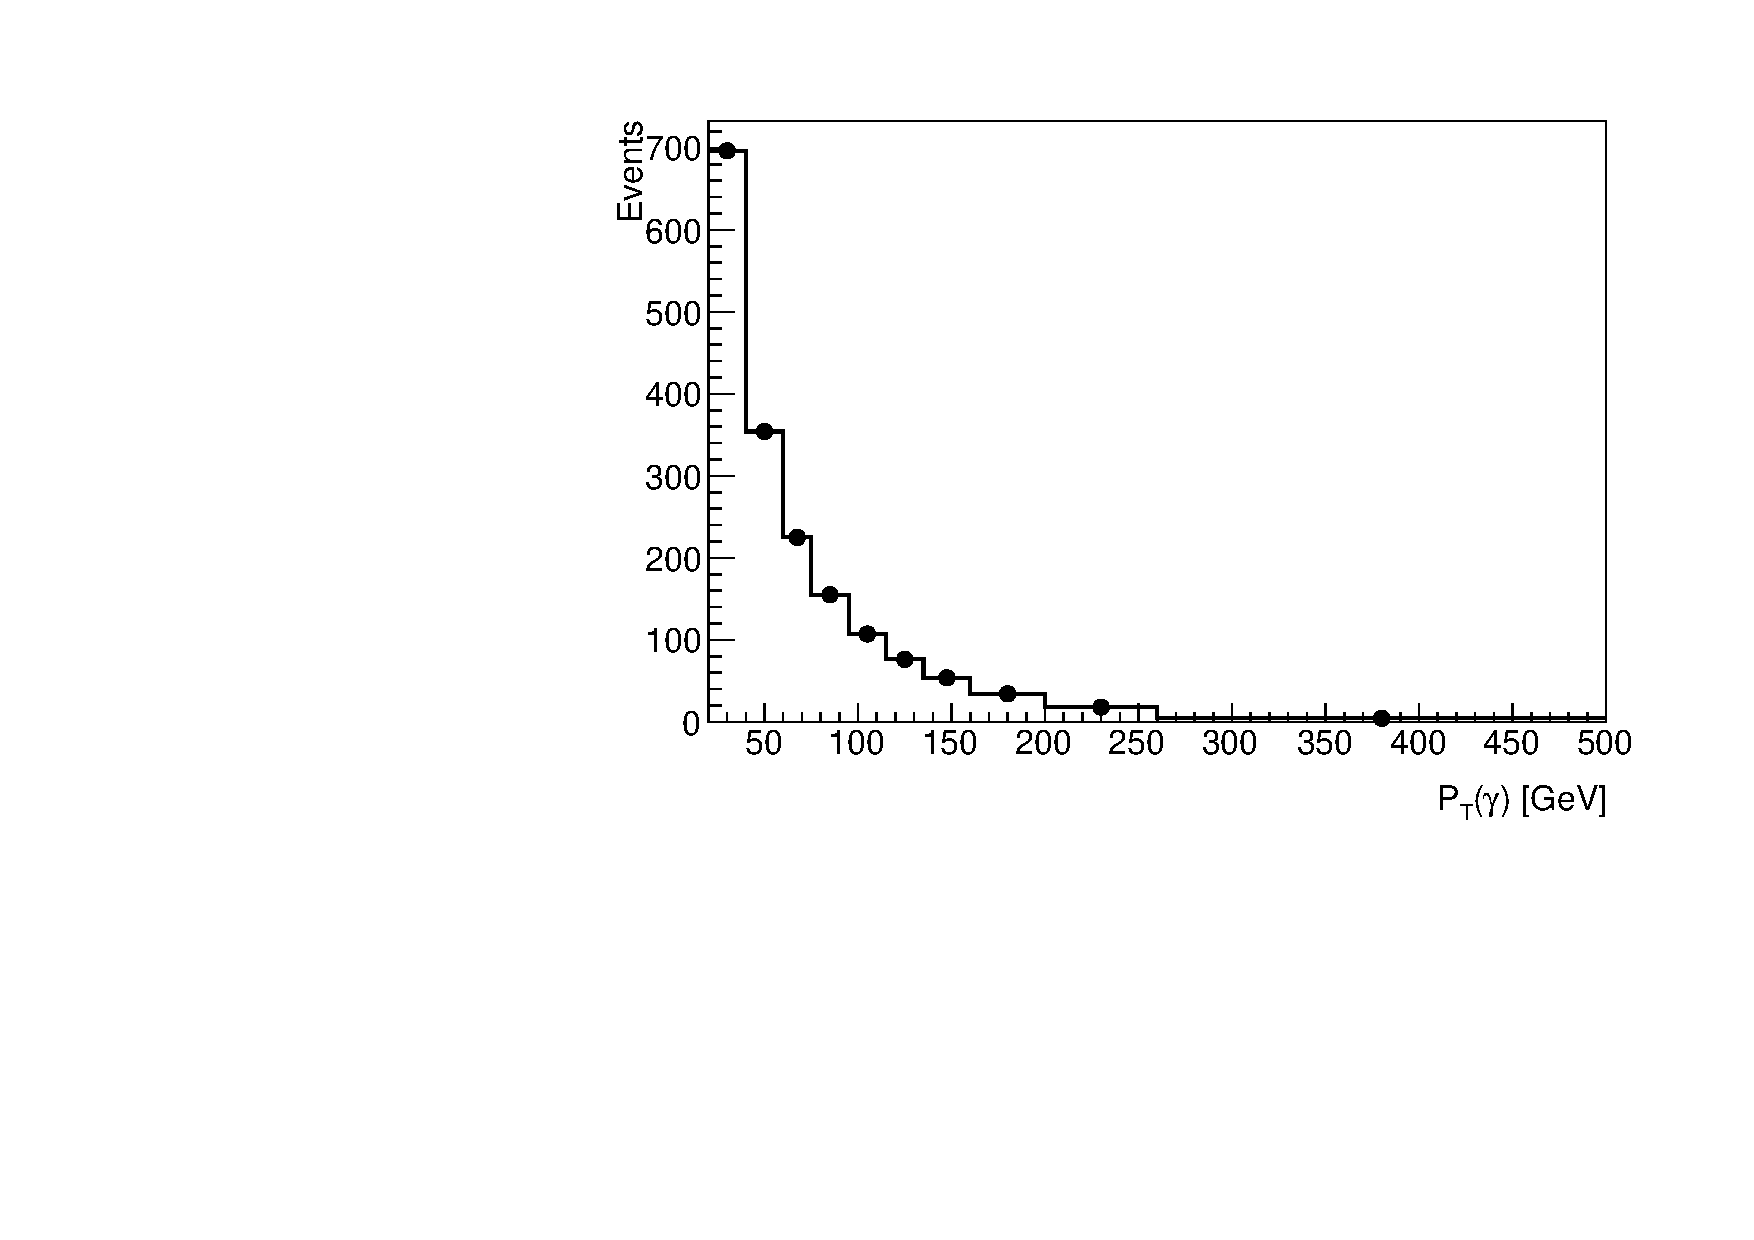
\includegraphics[width=0.4\textwidth]{figures/diff_xsec/ljet/Truth_dist/tty1l_pt_all_syst_Unfolding_truth_distribution.pdf}}
    \quad \quad
    % ph eta
    \subfloat[]{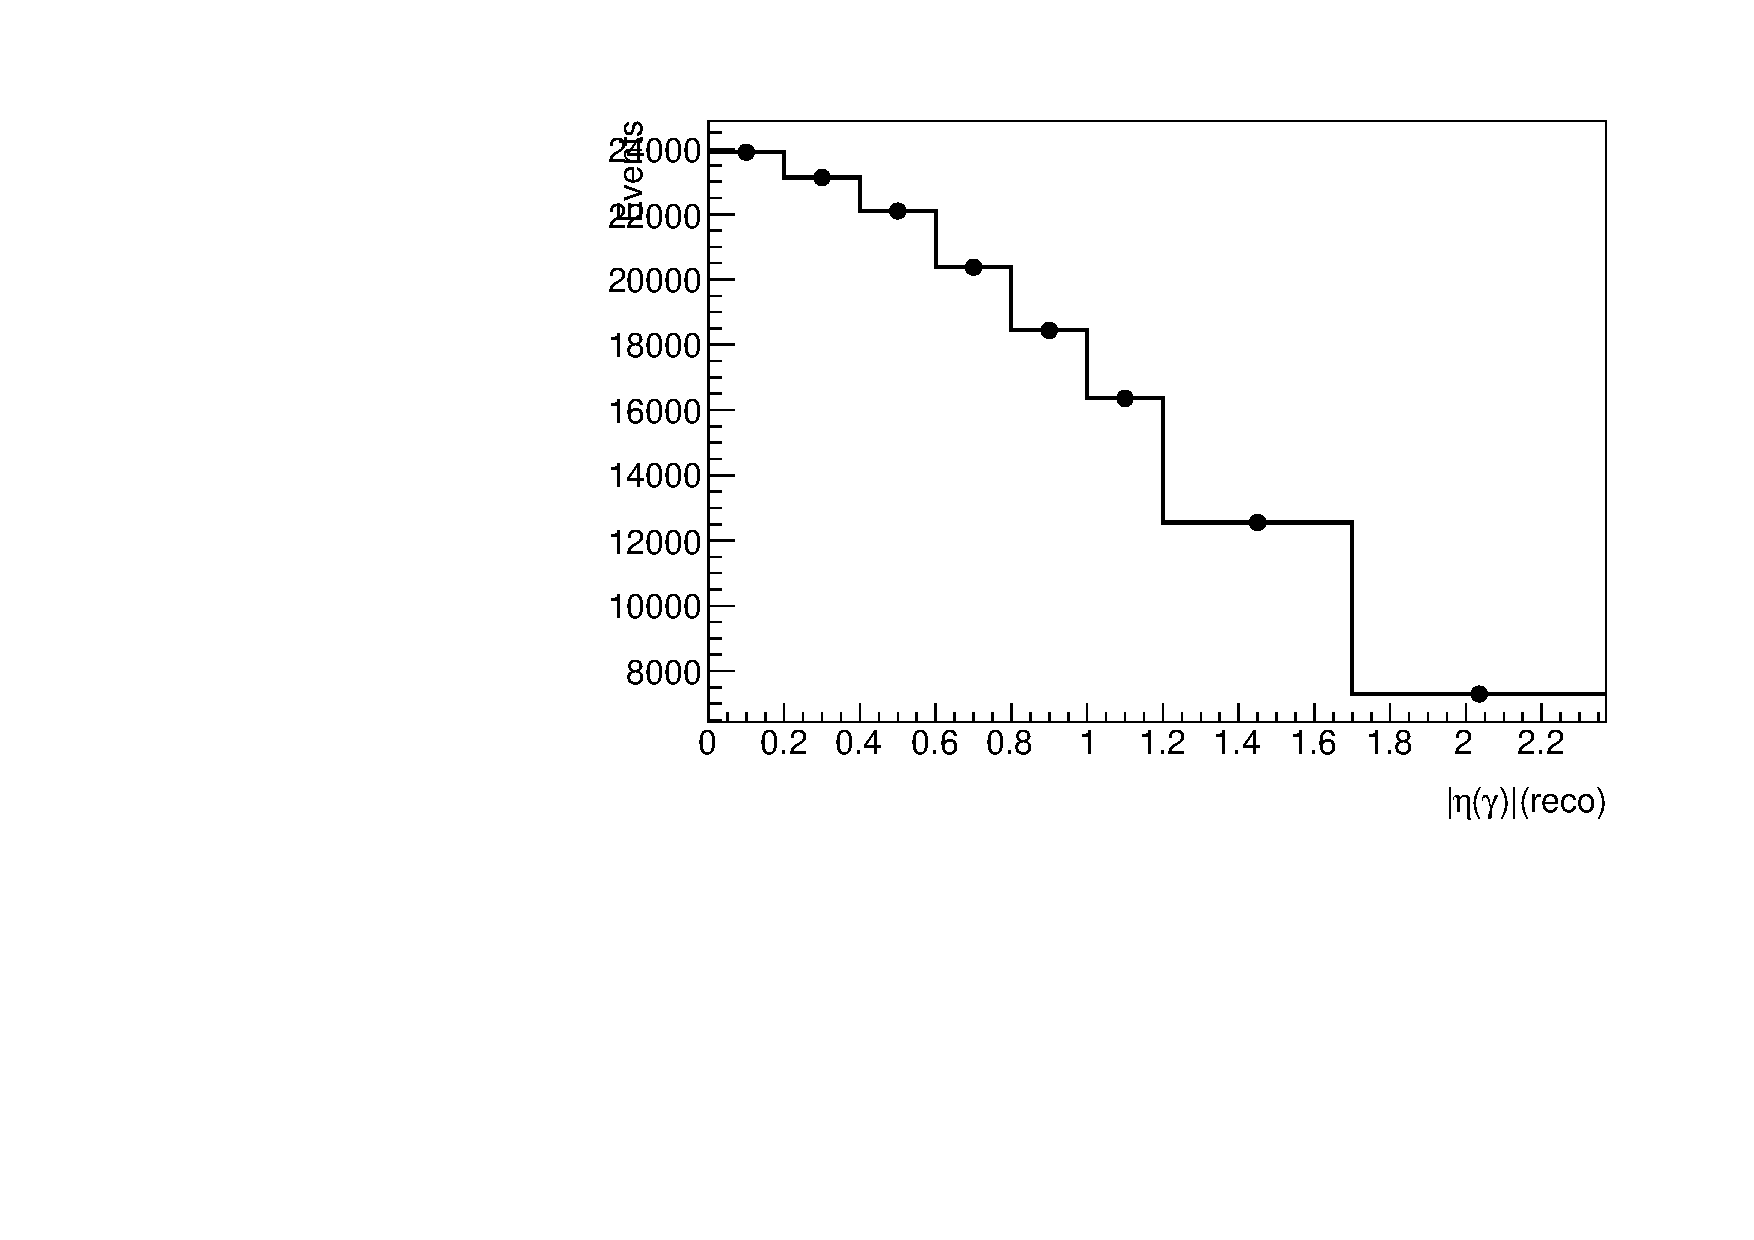
\includegraphics[width=0.4\textwidth]{figures/diff_xsec/ljet/Truth_dist/tty1l_eta_all_syst_Unfolding_truth_distribution.pdf}}
    \quad \quad
    % delta R (ph, l)
    \subfloat[]{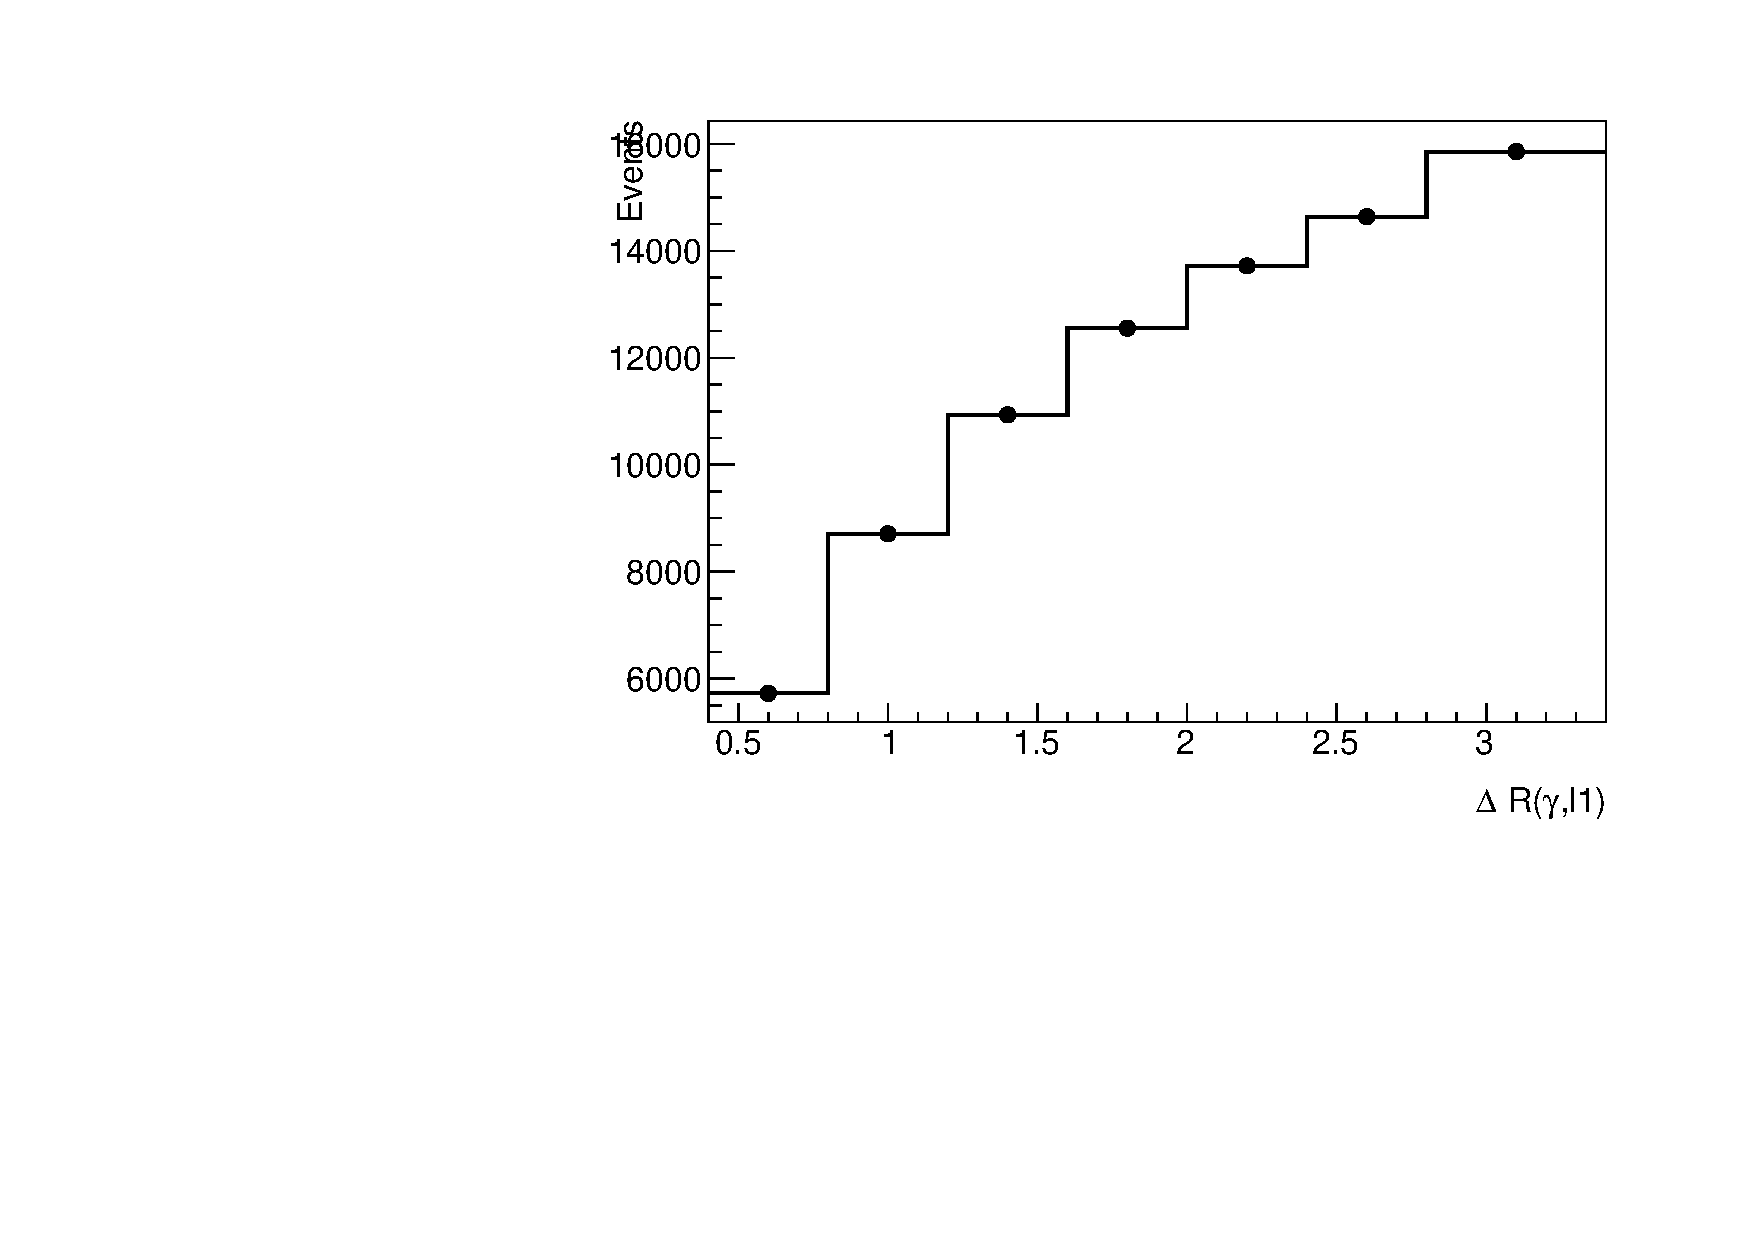
\includegraphics[width=0.4\textwidth]{figures/diff_xsec/ljet/Truth_dist/tty1l_dr_all_syst_Unfolding_truth_distribution.pdf}}
    \quad \quad
    % delta R (ph, b)
    \subfloat[]{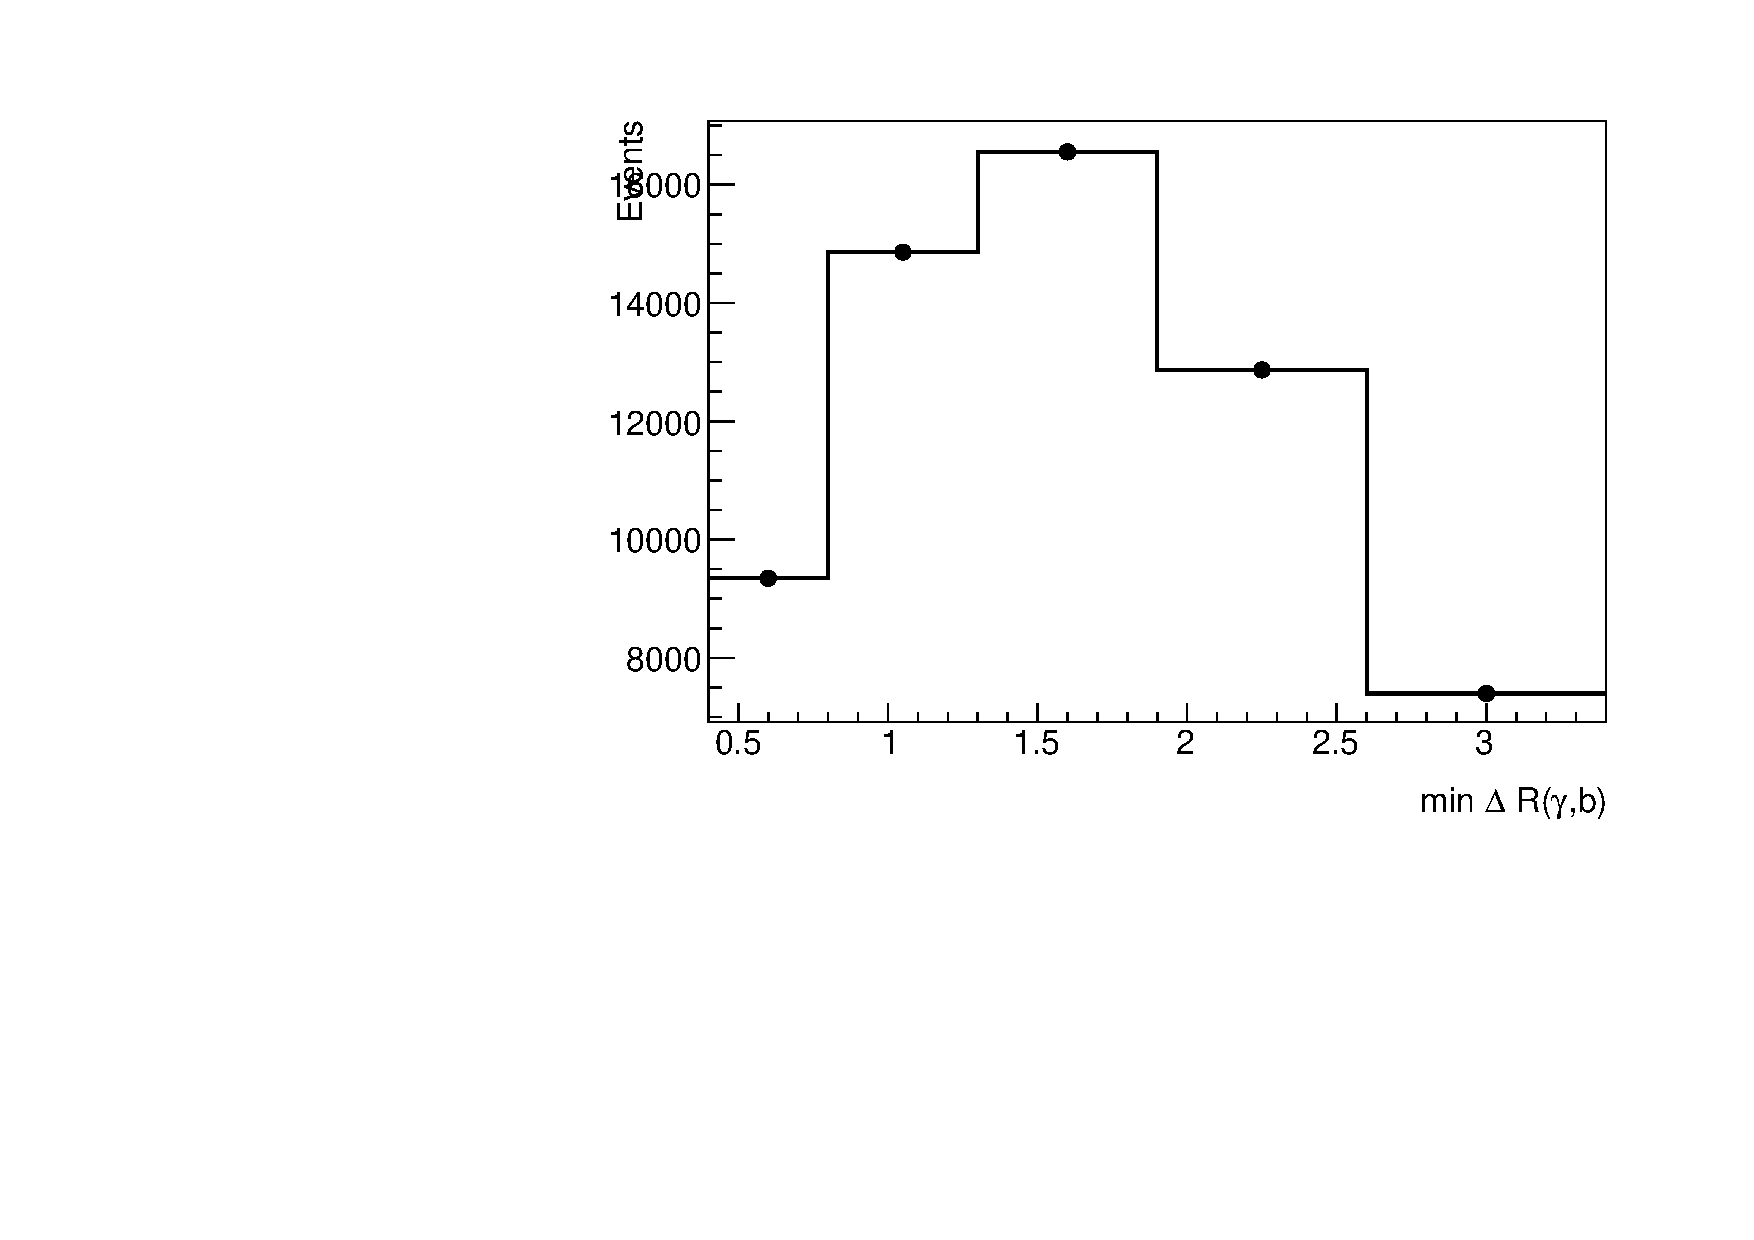
\includegraphics[width=0.4\textwidth]{figures/diff_xsec/ljet/Truth_dist/tty1l_drphb_all_syst_Unfolding_truth_distribution.pdf}}
    \quad \quad
    % delta R(lj)
    \subfloat[]{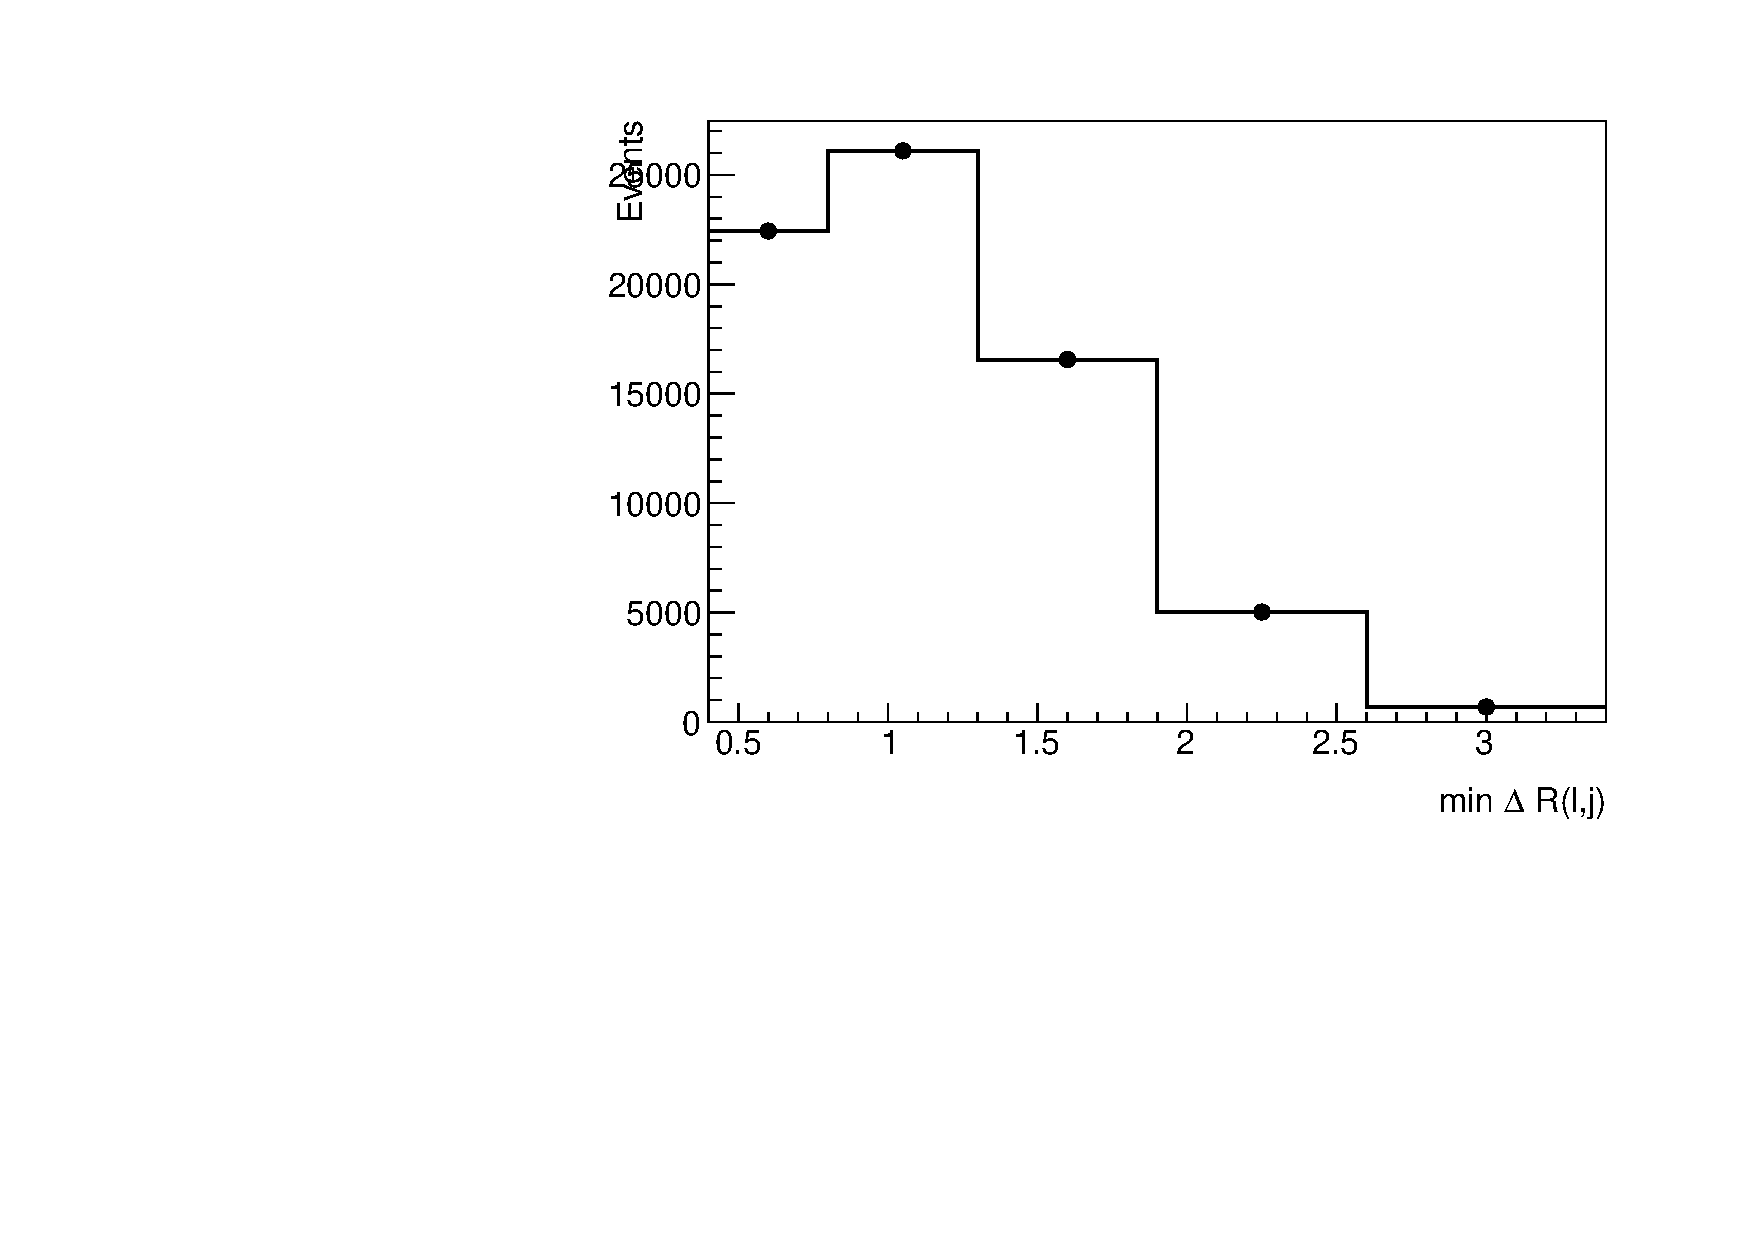
\includegraphics[width=0.4\textwidth]{figures/diff_xsec/ljet/Truth_dist/tty1l_drlj_all_syst_Unfolding_truth_distribution.pdf}}
    % pt j1
    \subfloat[]{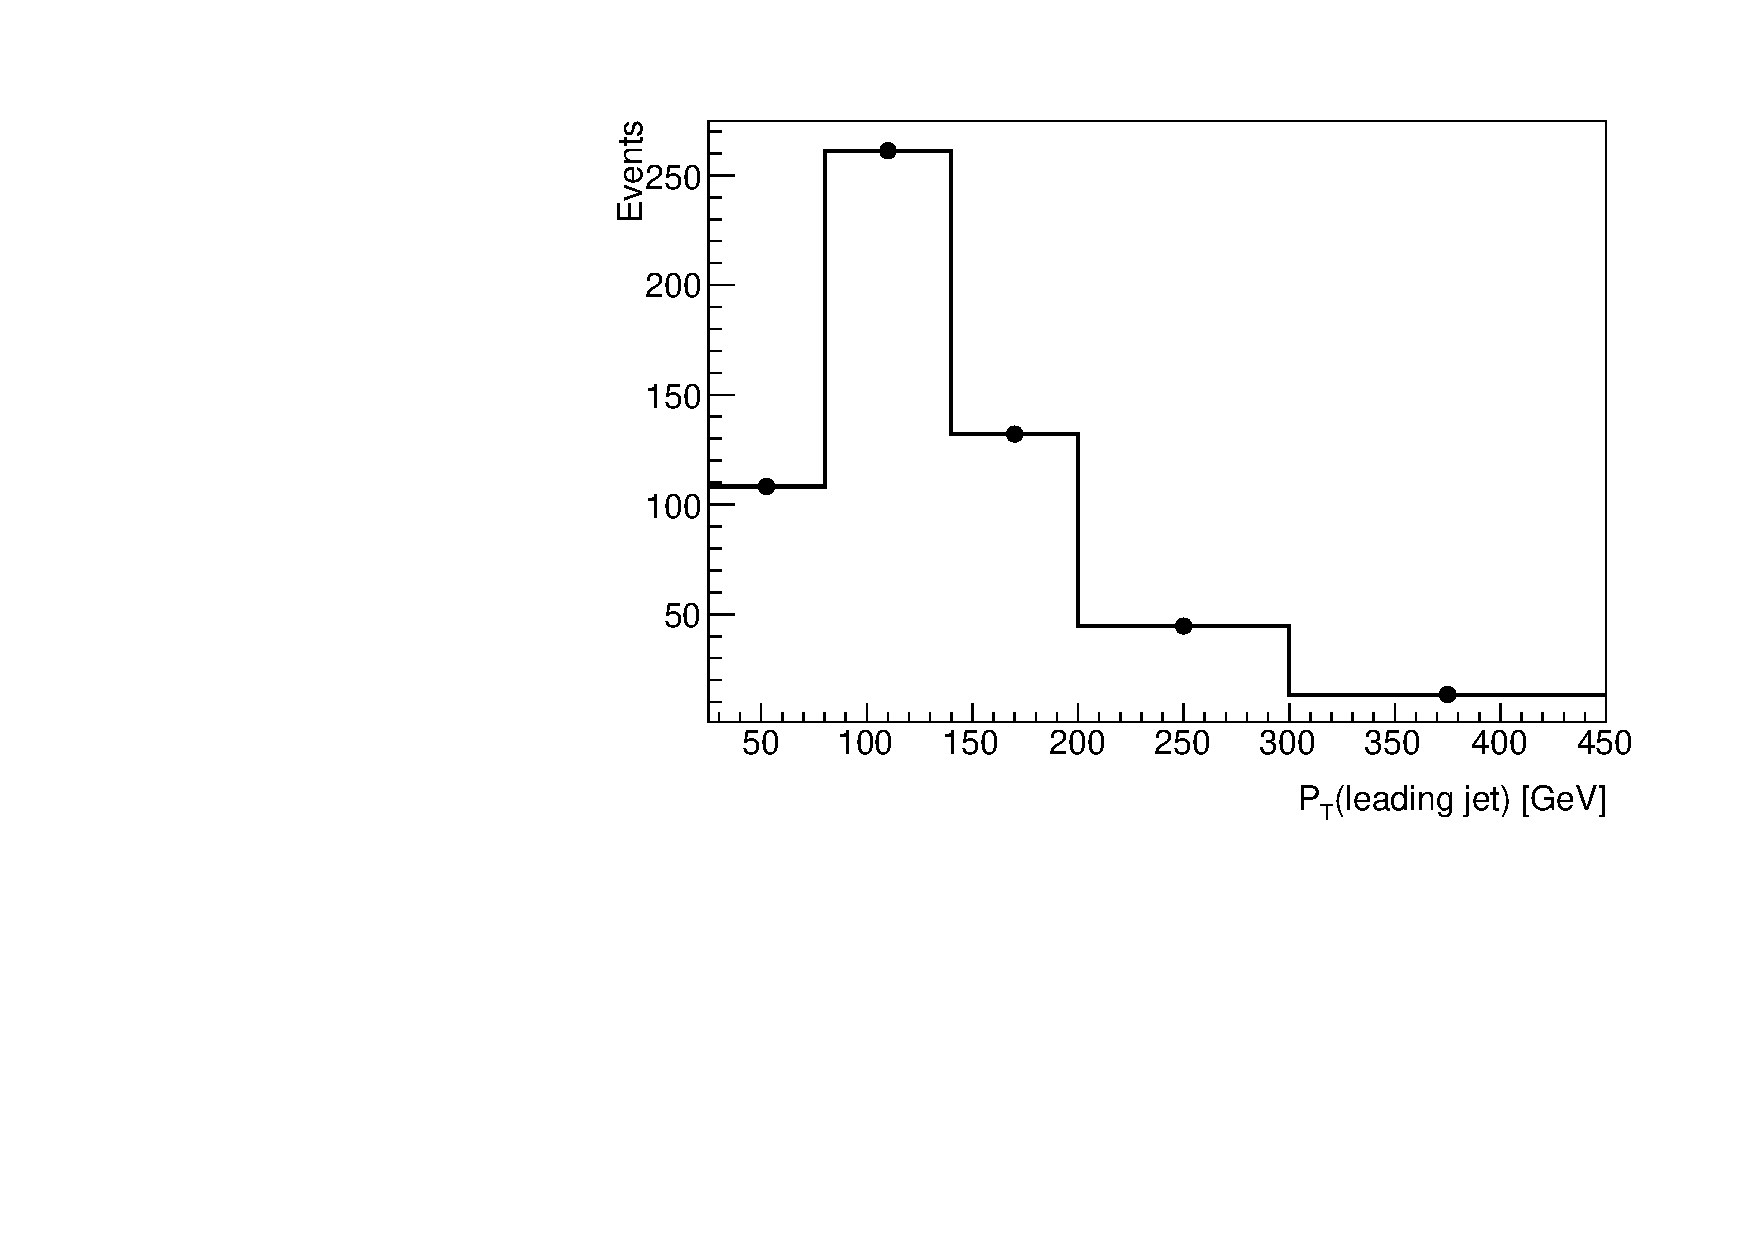
\includegraphics[width=0.4\textwidth]{figures/diff_xsec/ljet/Truth_dist/tty1l_ptj1_all_syst_Unfolding_truth_distribution.pdf}}
    \caption{The particle level distribution of $t\bar{t}\gamma$ (prod) (MC signal) for different observables in the single lepton channel. Number of events corresponds to the expected number of events at particle level normalised to the luminosity of data. Overflow events are included in the last bin of the corresponding distribution.
    Note that values are divided bin width.}
    \label{fig:folding_input_ljet}
\end{figure}
\FloatBarrier

\begin{figure}[ht]
    \centering
    % ph pt
    \subfloat[]{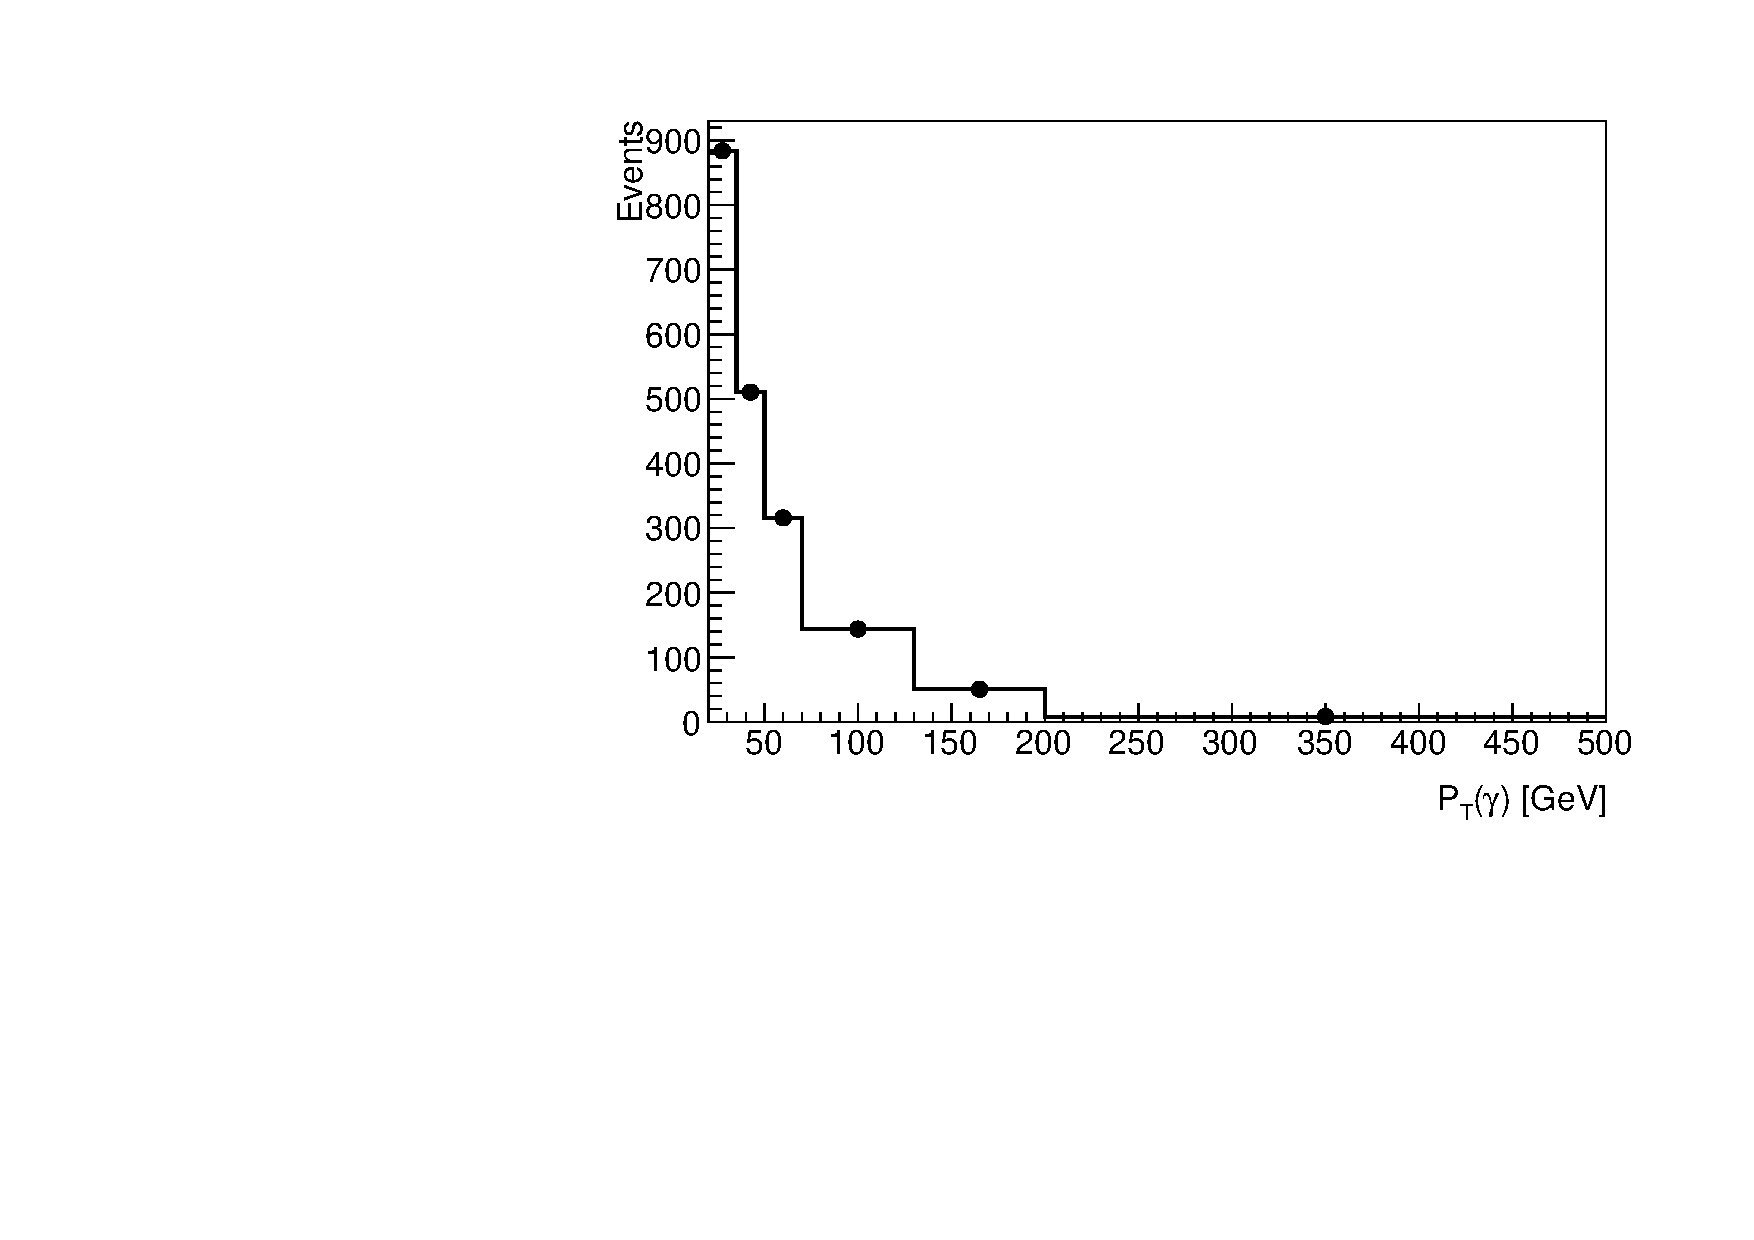
\includegraphics[width=0.4\textwidth]{figures/diff_xsec/dilep/Truth_dist/tty2l_pt_all_syst_Unfolding_truth_distribution.pdf}}
    \quad \quad
    % ph eta
    \subfloat[]{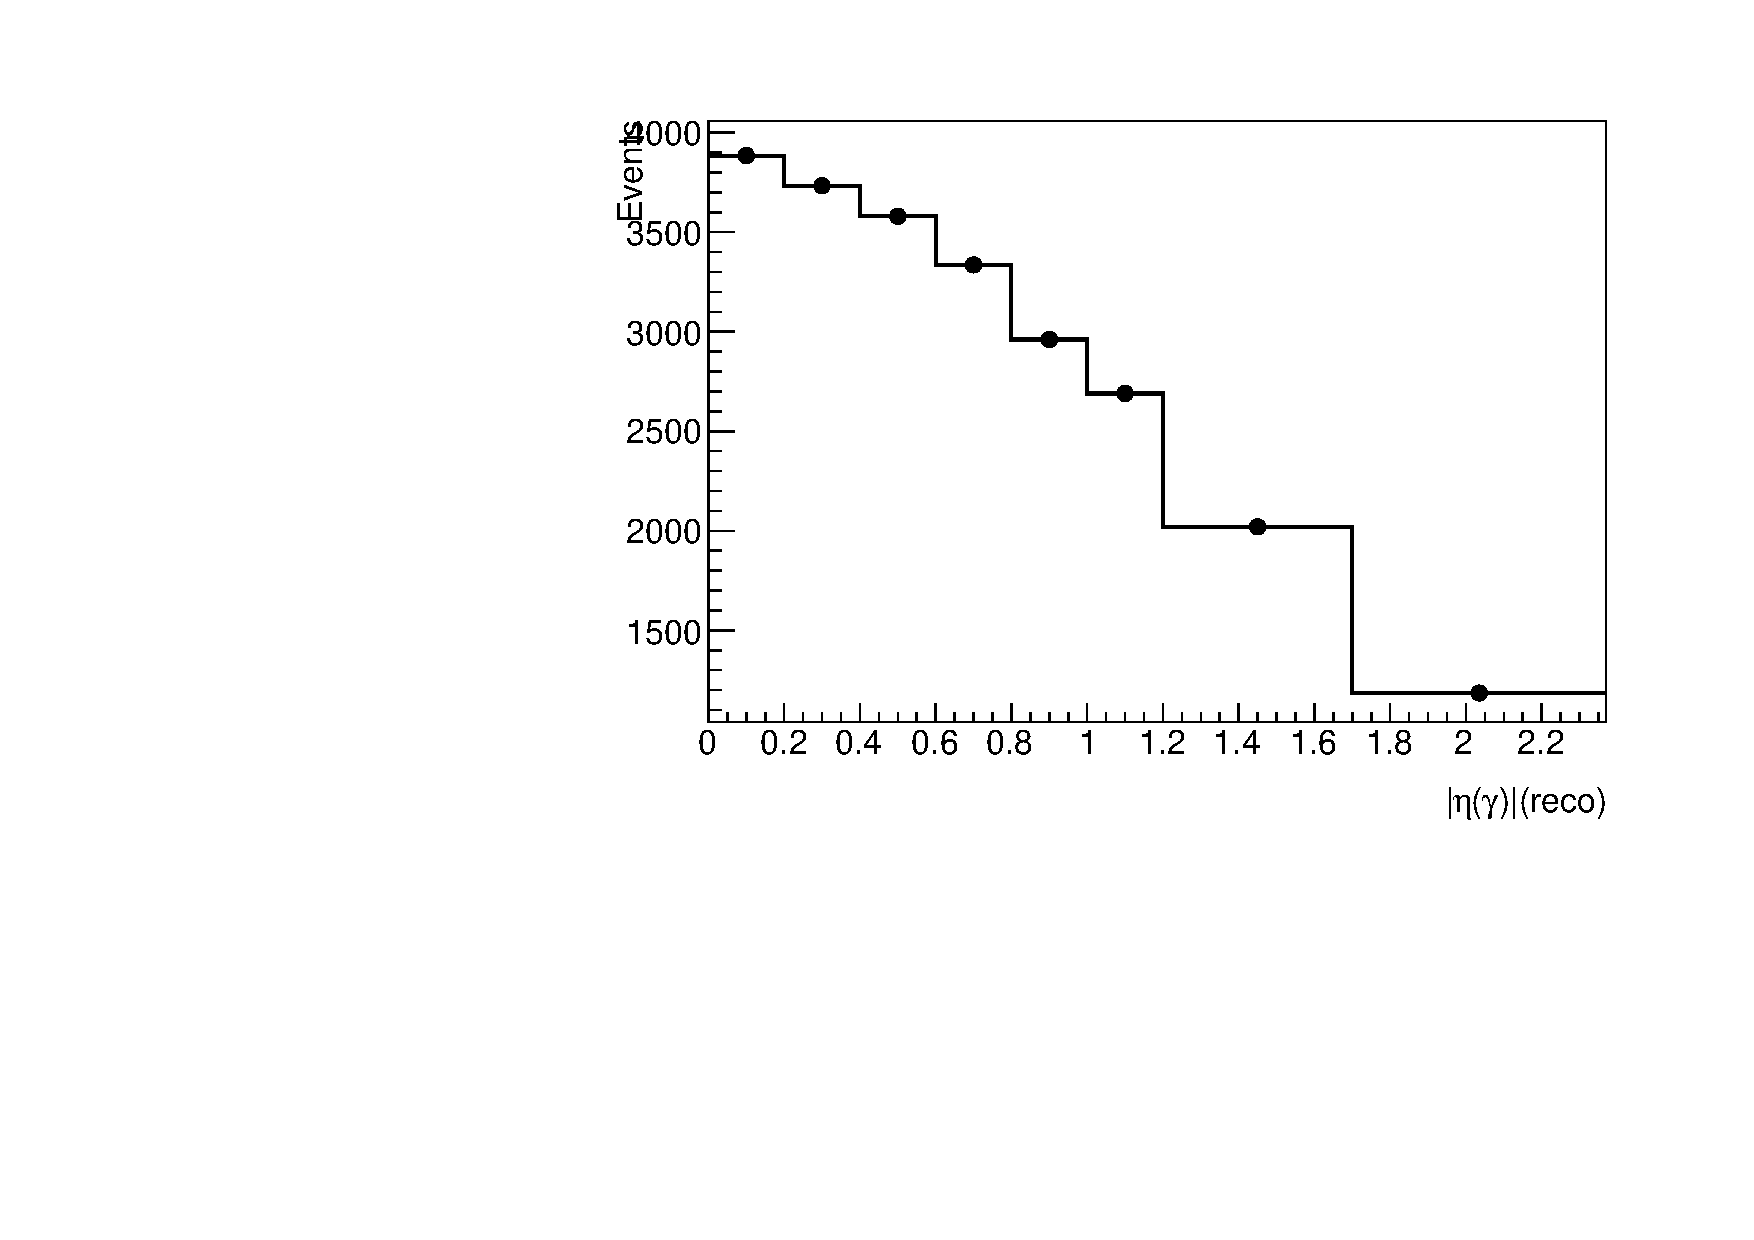
\includegraphics[width=0.4\textwidth]{figures/diff_xsec/dilep/Truth_dist/tty2l_eta_all_syst_Unfolding_truth_distribution.pdf}}
    \quad \quad
    % delta R (ph, l)
    \subfloat[]{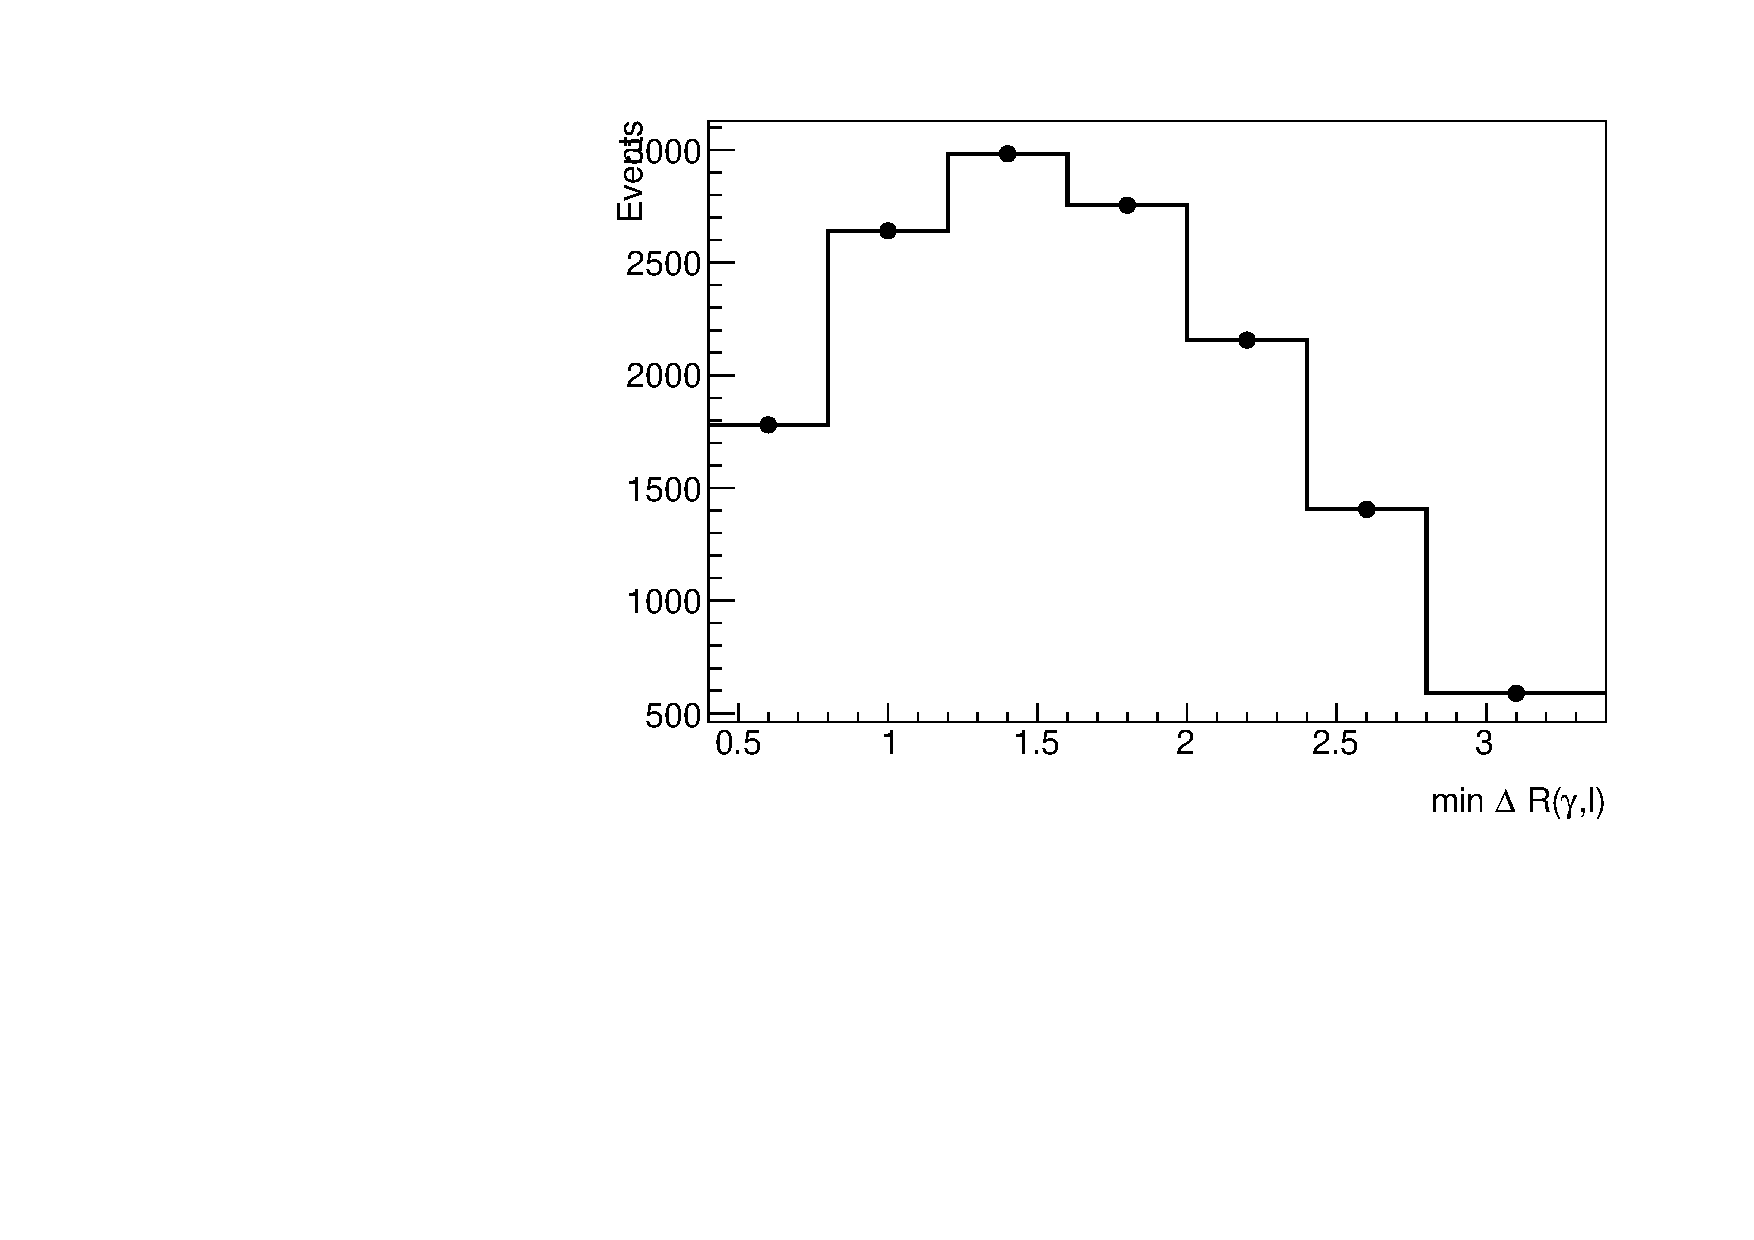
\includegraphics[width=0.4\textwidth]{figures/diff_xsec/dilep/Truth_dist/tty2l_dr_all_syst_Unfolding_truth_distribution.pdf}}
    \quad \quad
    % delta R (ph, l1)
    \subfloat[]{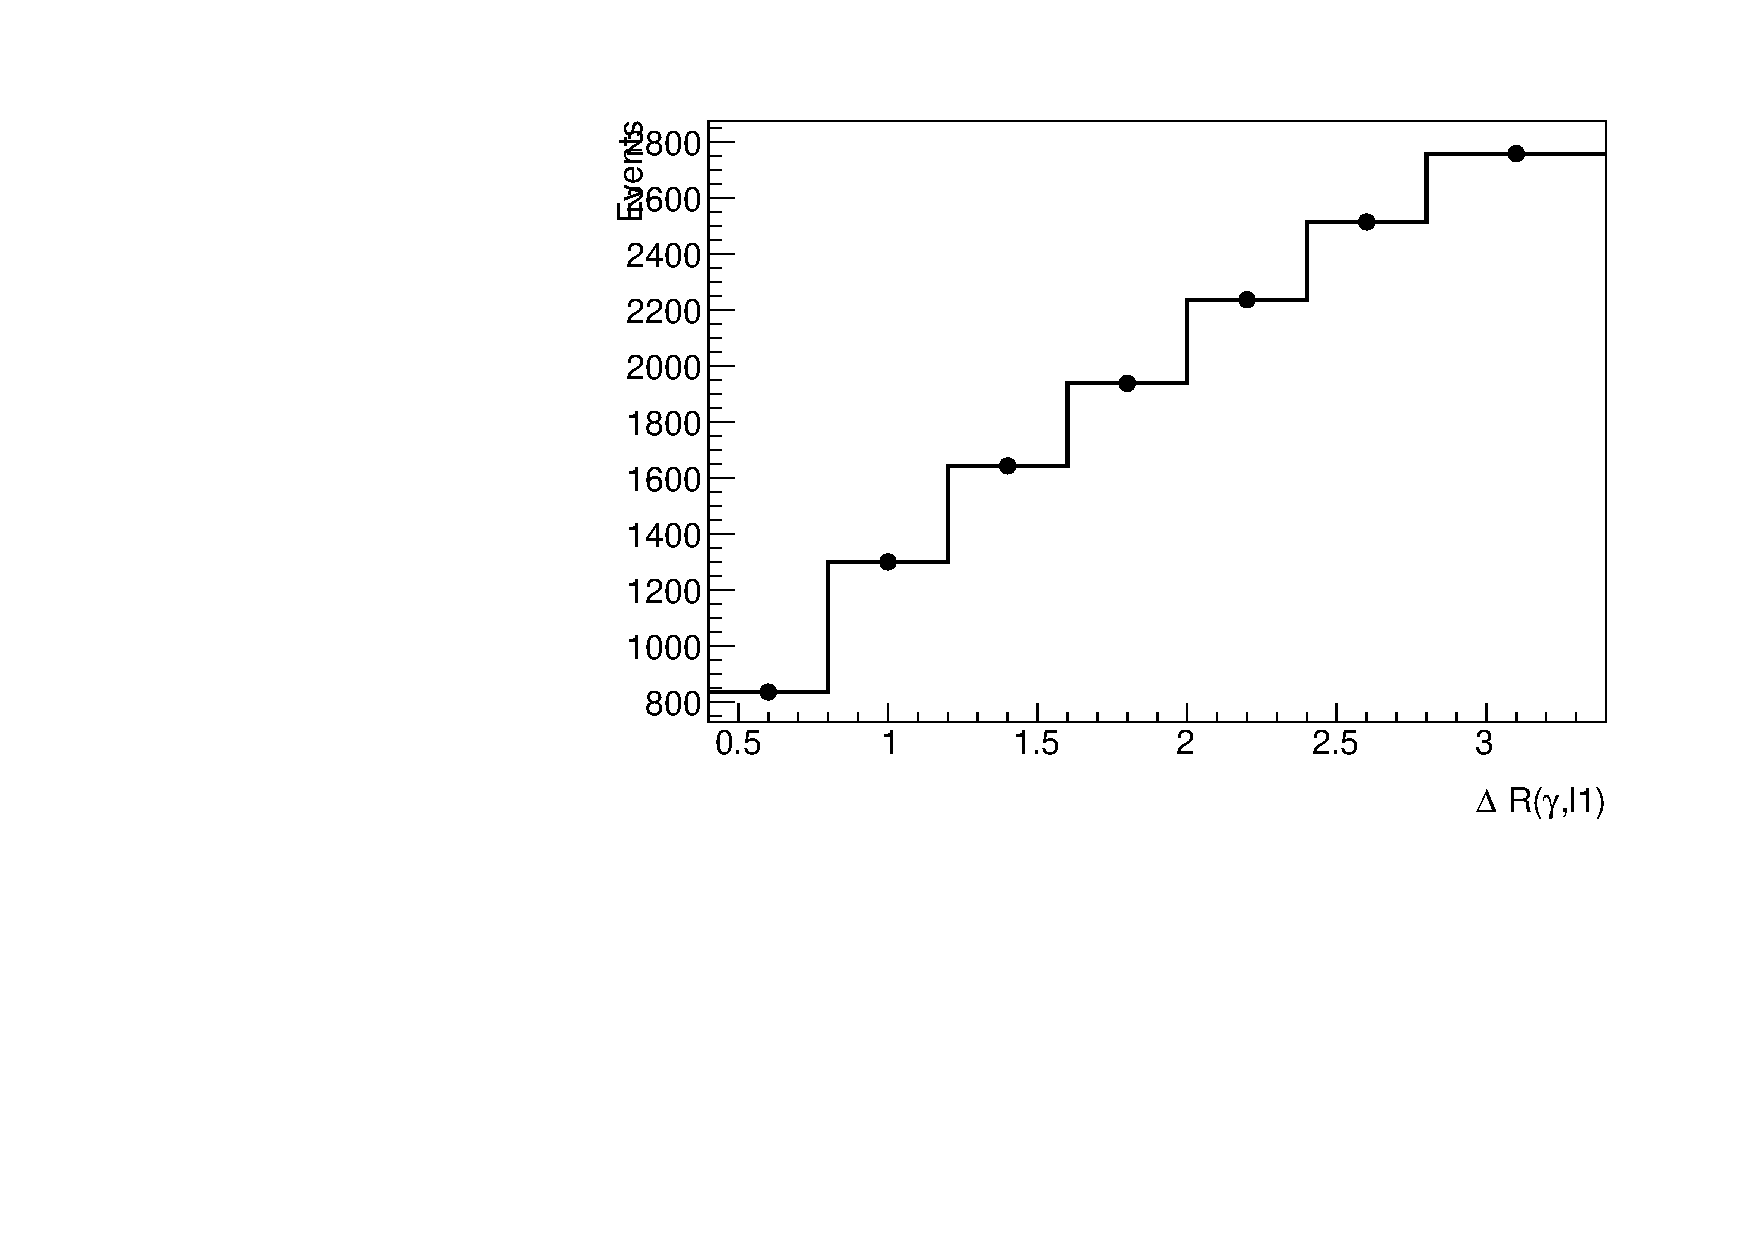
\includegraphics[width=0.4\textwidth]{figures/diff_xsec/dilep/Truth_dist/tty2l_dr1_all_syst_Unfolding_truth_distribution.pdf}}
    \quad \quad
    % delta R (ph, l2)
    \subfloat[]{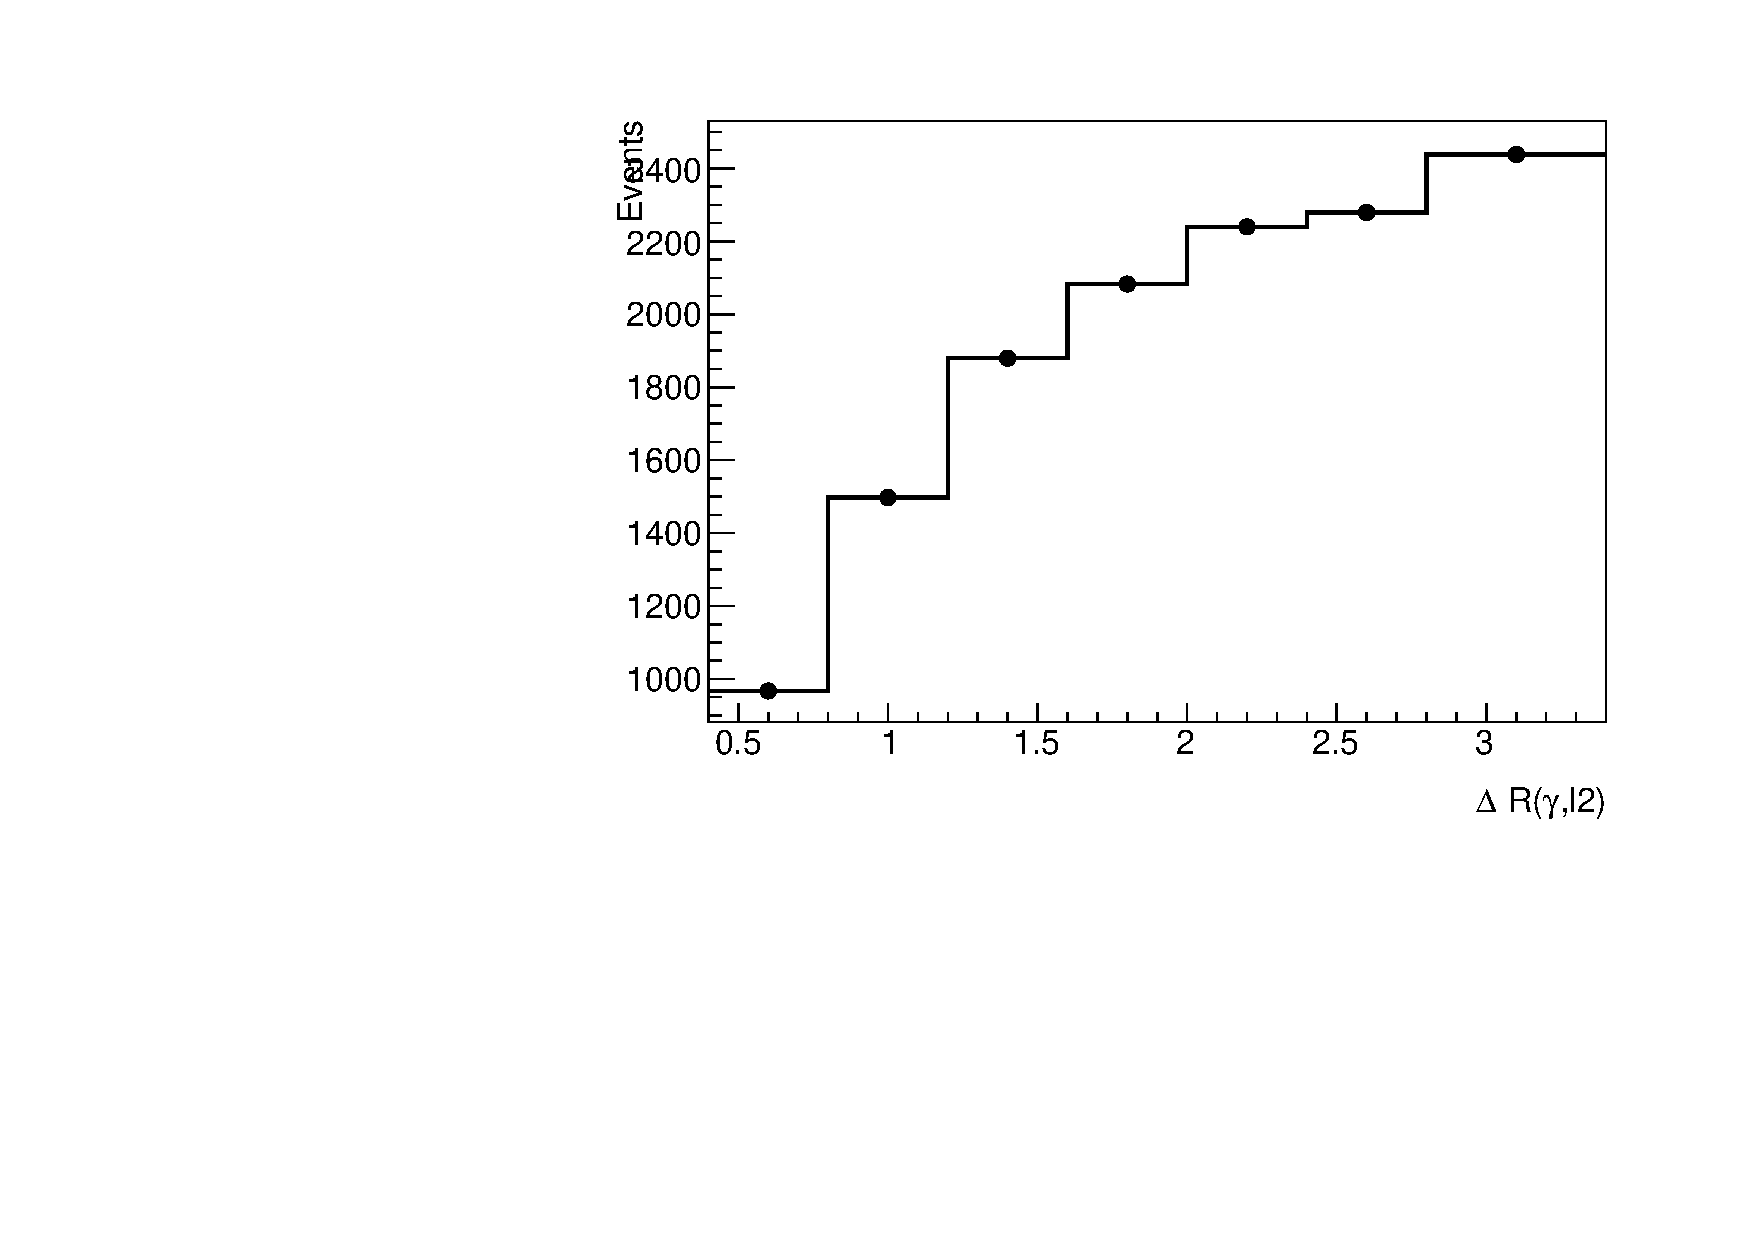
\includegraphics[width=0.4\textwidth]{figures/diff_xsec/dilep/Truth_dist/tty2l_dr2_all_syst_Unfolding_truth_distribution.pdf}}
    \quad \quad
    % delta R (ph, b)
    \subfloat[]{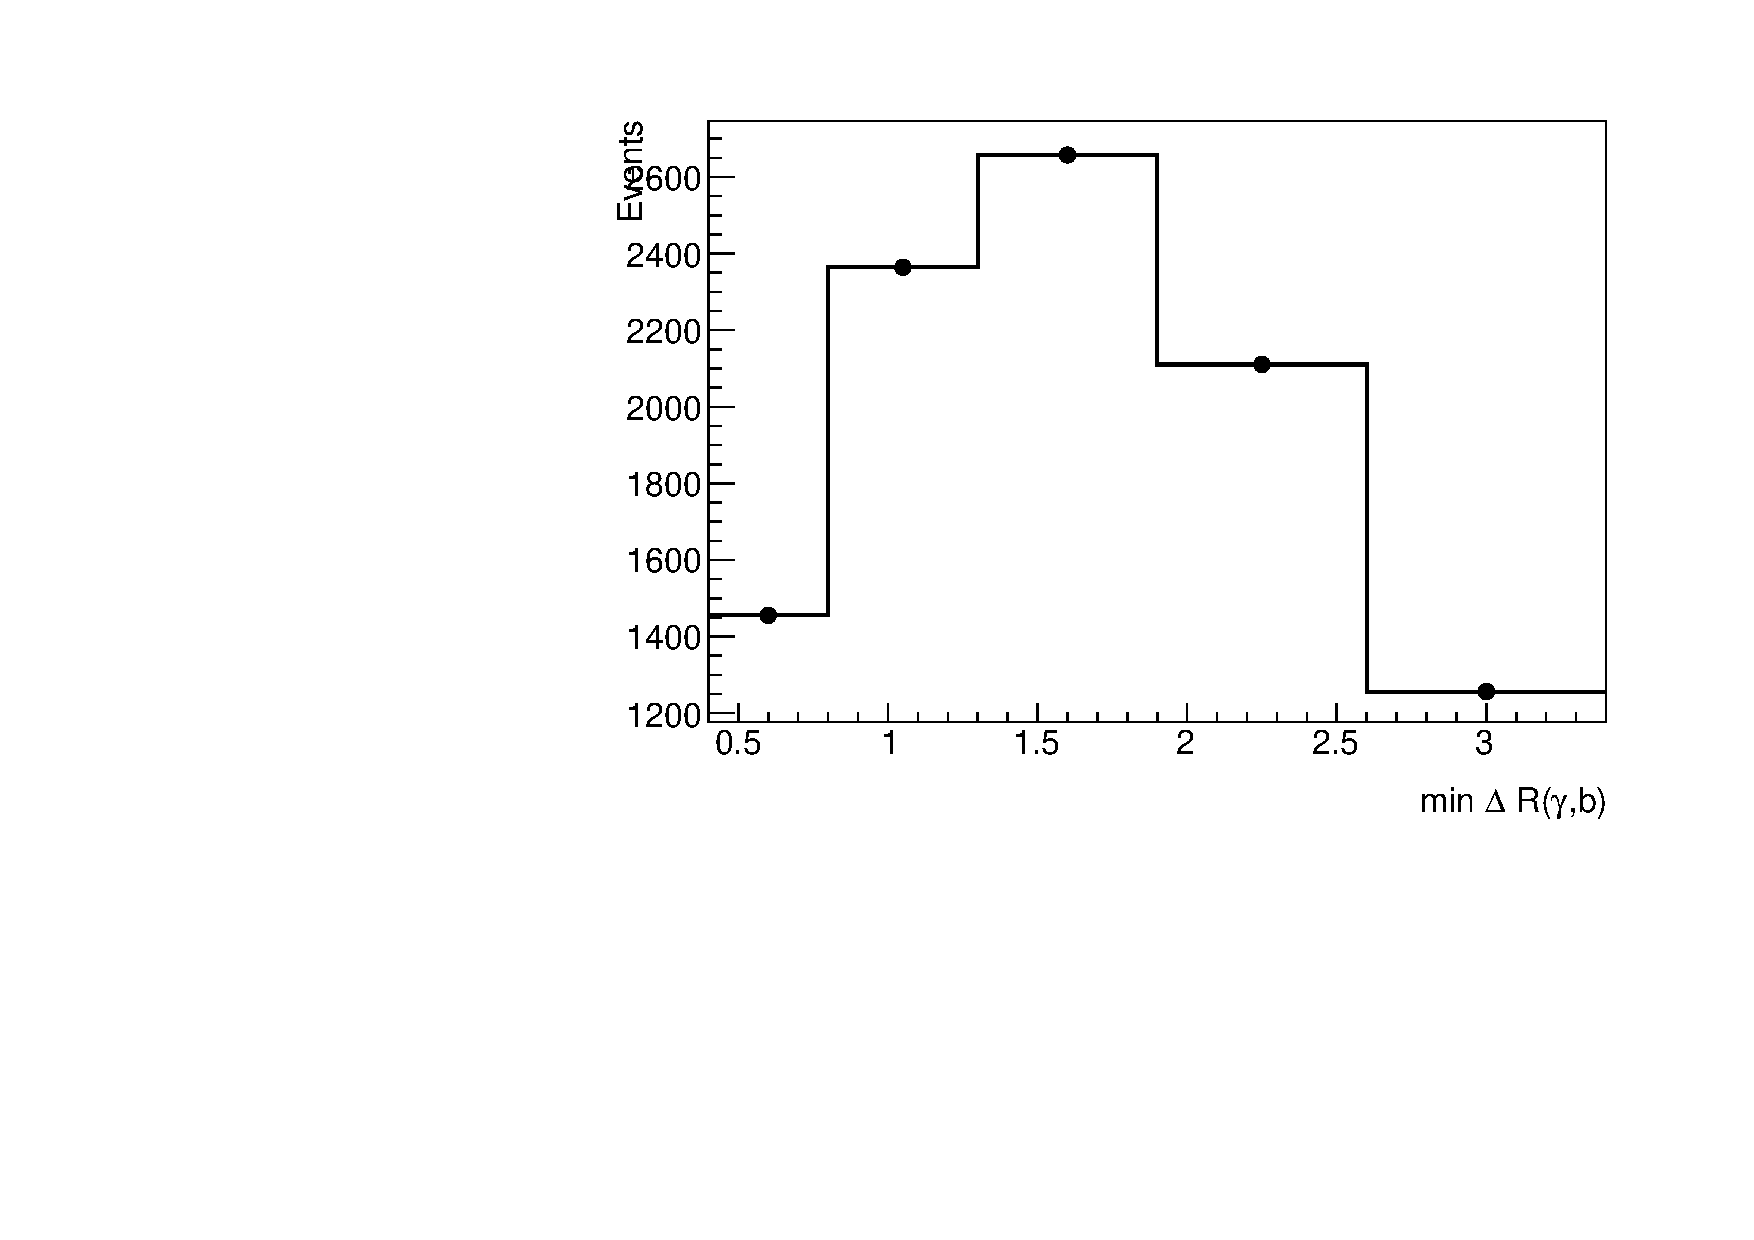
\includegraphics[width=0.4\textwidth]{figures/diff_xsec/dilep/Truth_dist/tty2l_drphb_all_syst_Unfolding_truth_distribution.pdf}}
    \quad \quad
    % dEta(ll)
    \subfloat[]{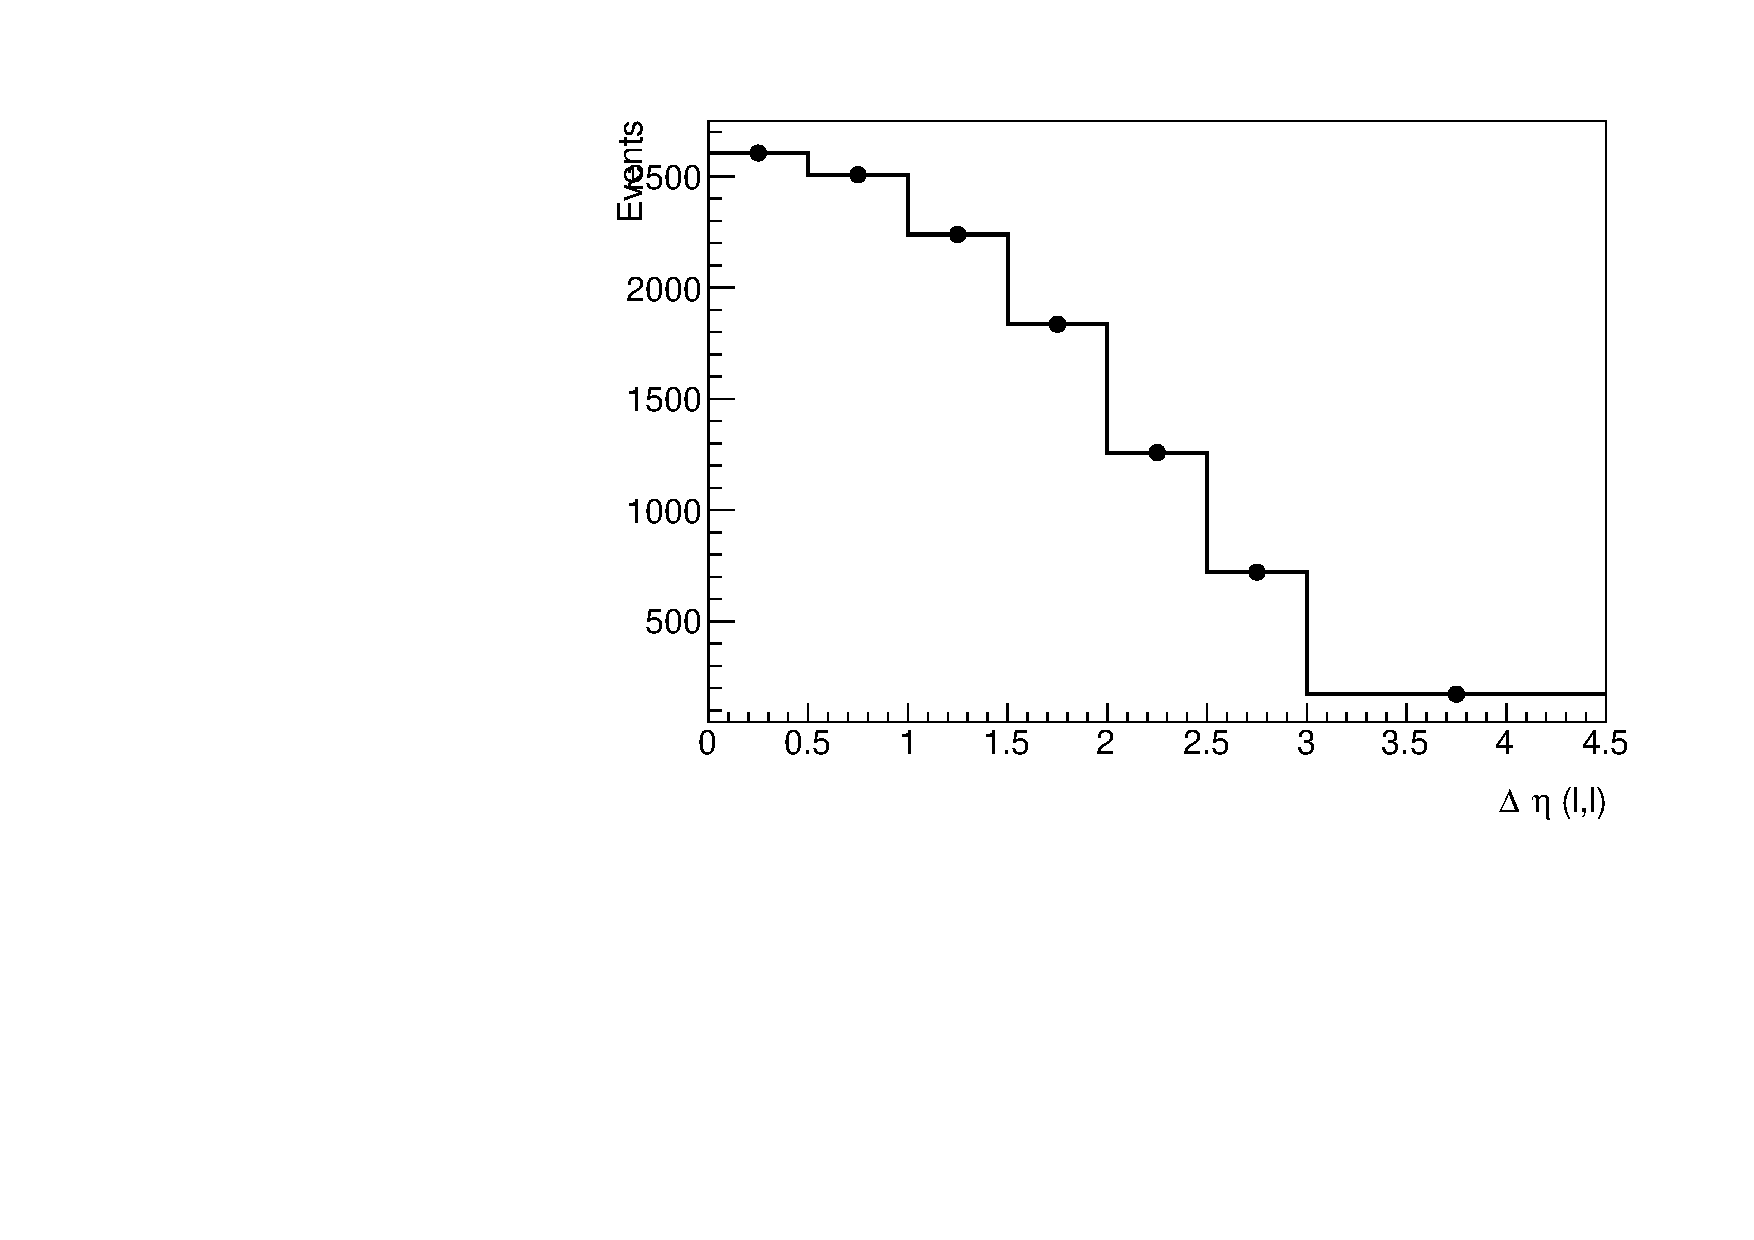
\includegraphics[width=0.4\textwidth]{figures/diff_xsec/dilep/Truth_dist/tty2l_dEtall_all_syst_Unfolding_truth_distribution.pdf}}
    \caption{The particle level distribution of $t\bar{t}\gamma$ (prod) (MC signal) for different observables in the di-lepton channel. Number of events corresponds to the expected number of events at particle level normalised to the luminosity of data. Overflow events are included in the last bin of the corresponding distribution.
    Note that values are divided bin width.}
    \label{fig:folding_input_dilep1}
\end{figure}


\begin{figure}[ht]
    \centering
    \quad \quad
    % dPhi(ll)
    \subfloat[]{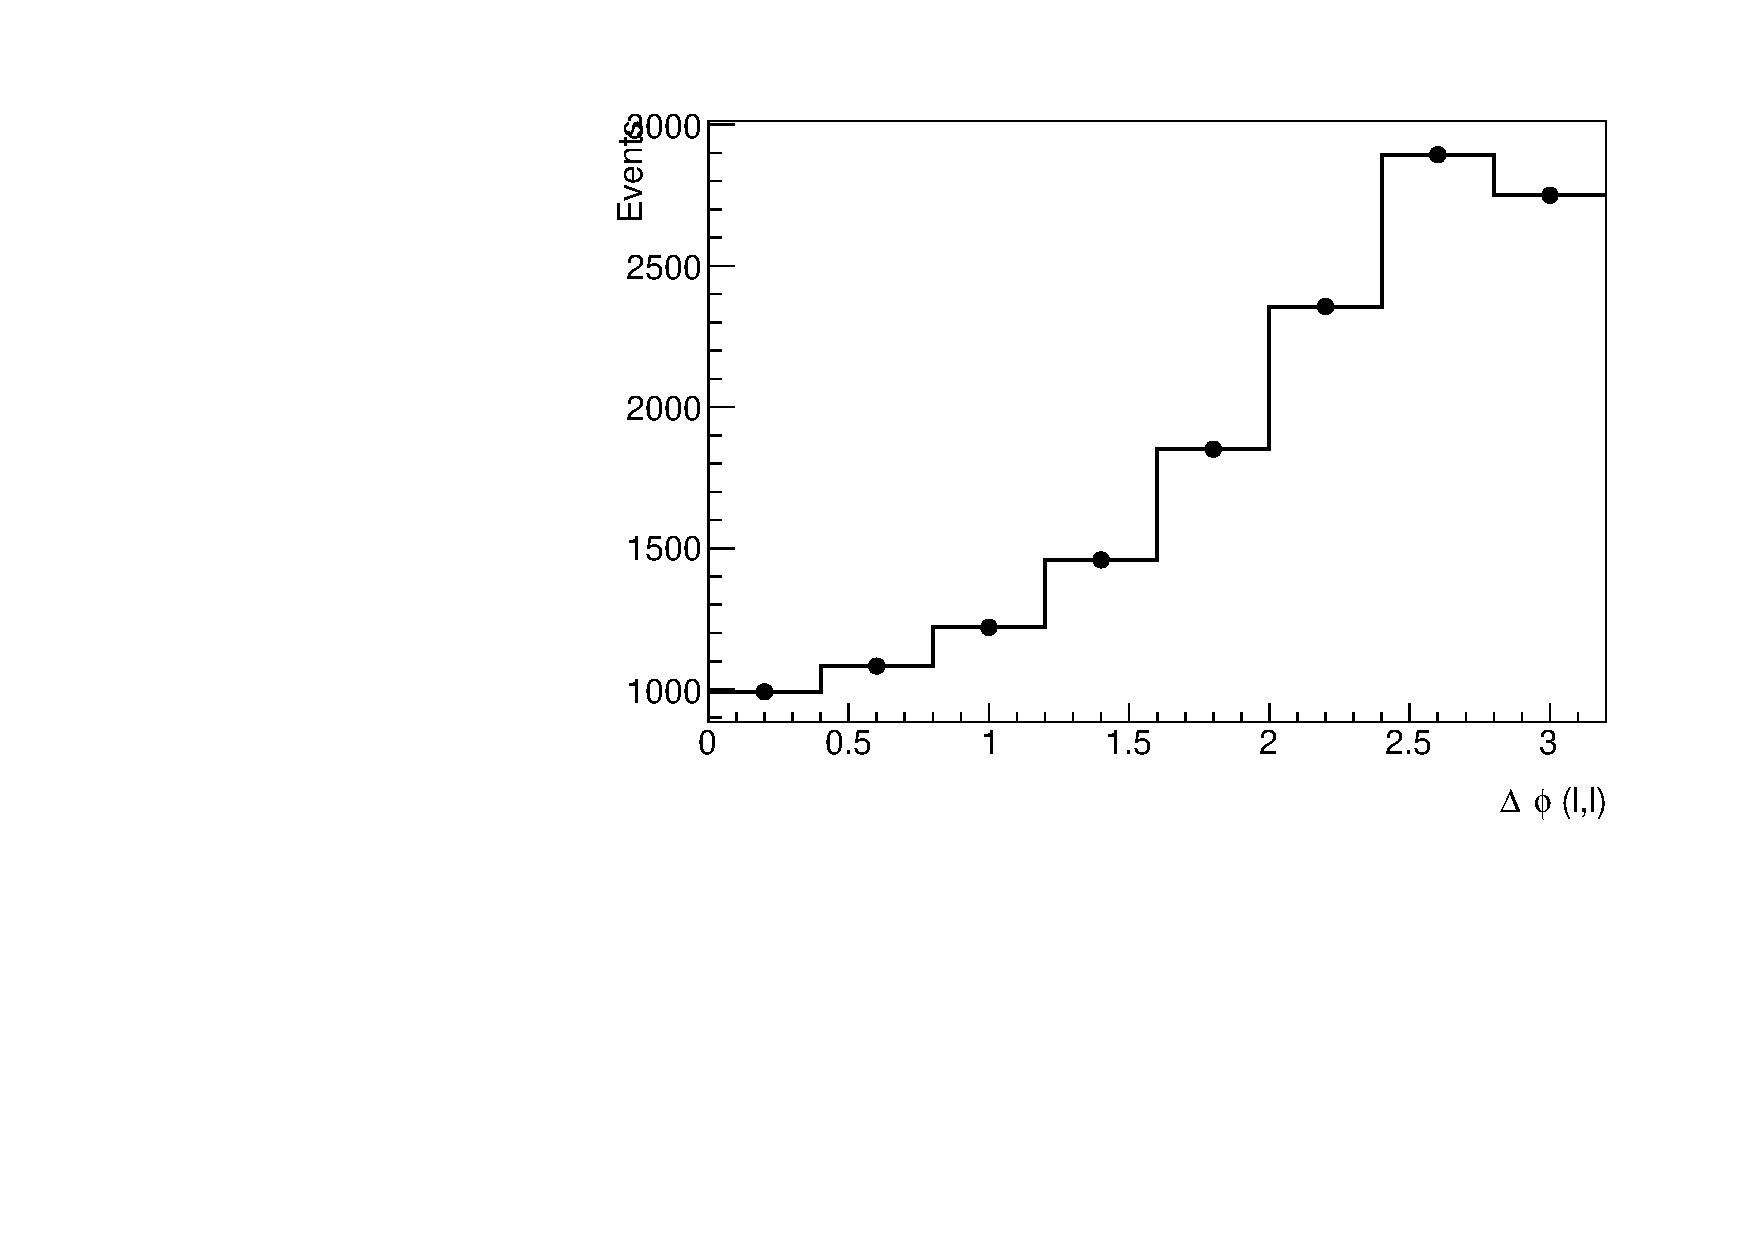
\includegraphics[width=0.4\textwidth]{figures/diff_xsec/dilep/Truth_dist/tty2l_dPhill_all_syst_Unfolding_truth_distribution.pdf}}
    % Pt(ll)
    \subfloat[]{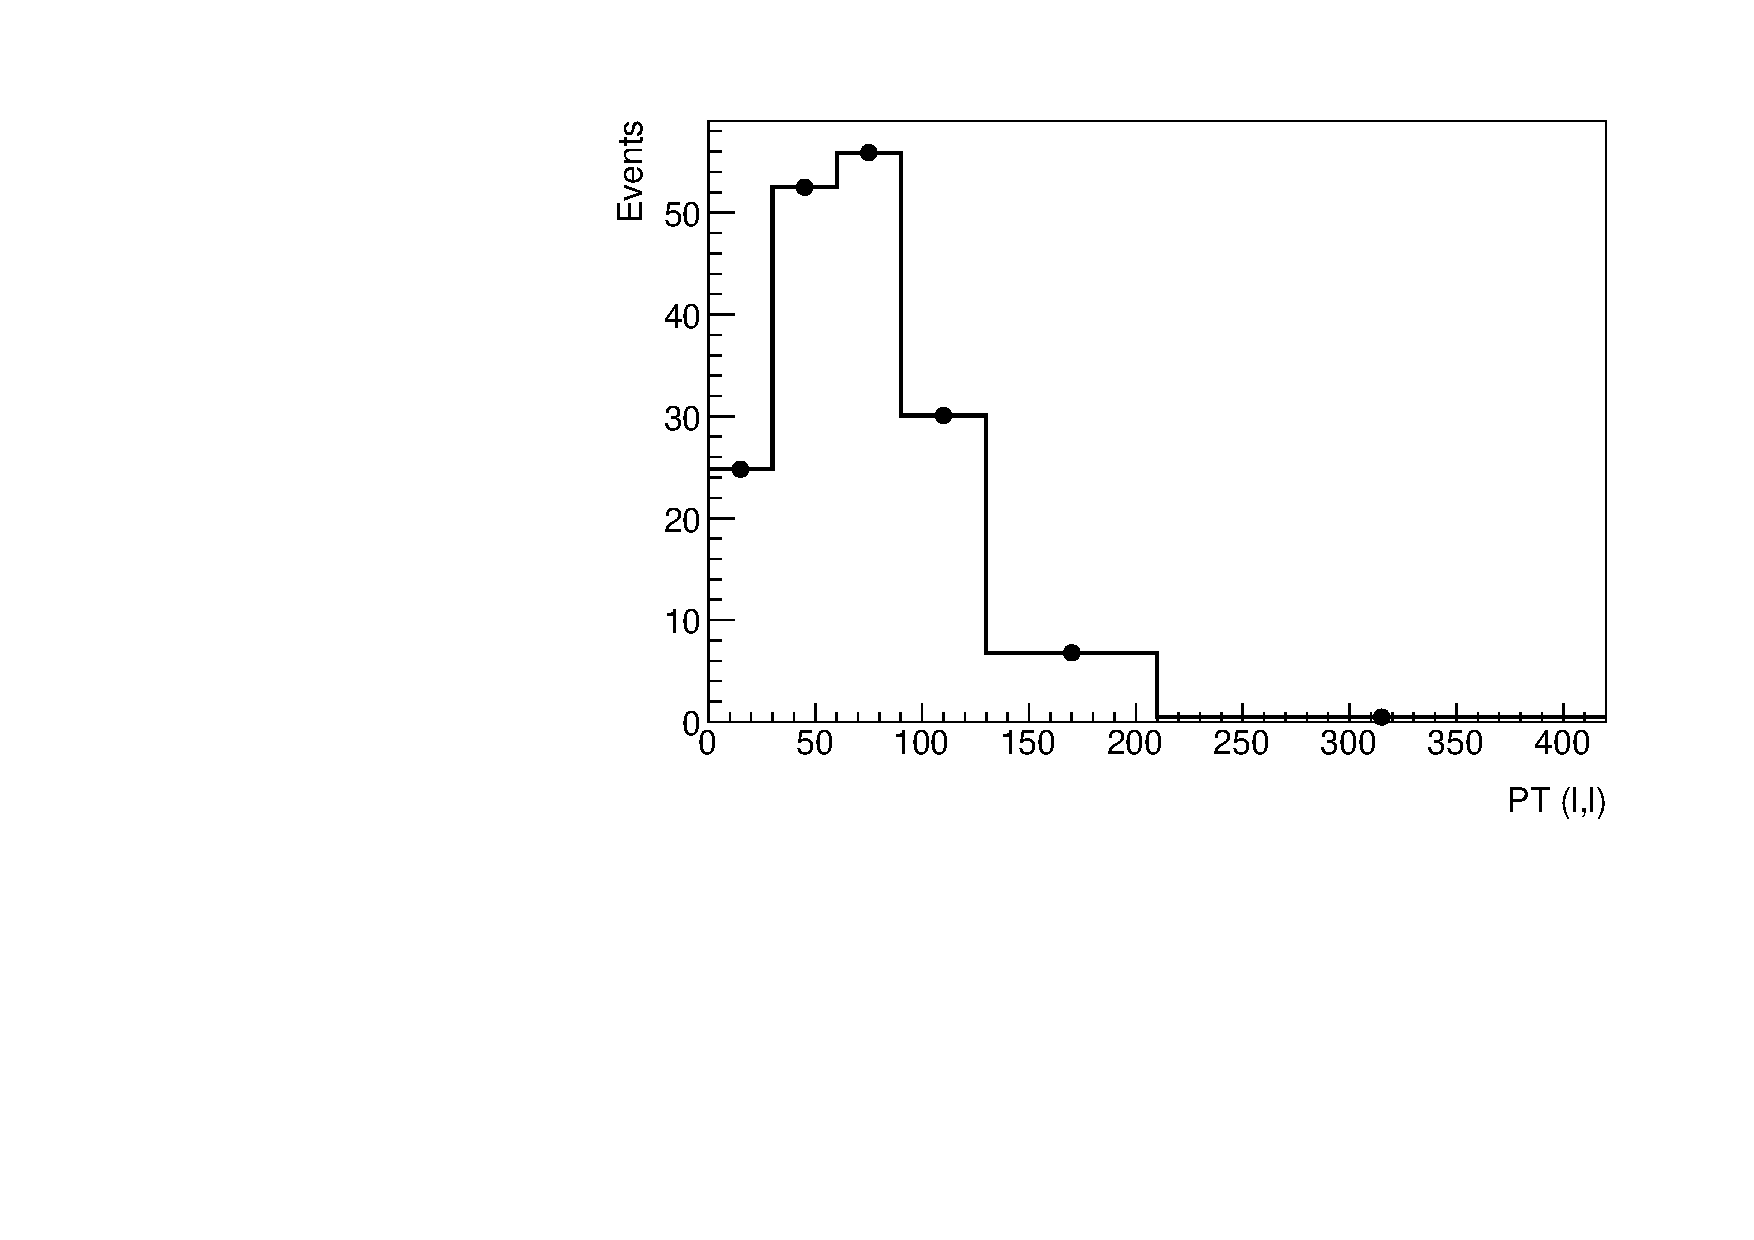
\includegraphics[width=0.4\textwidth]{figures/diff_xsec/dilep/Truth_dist/tty2l_ptll_all_syst_Unfolding_truth_distribution.pdf}}
    \quad \quad
    % Delta R (lj)
    \subfloat[]{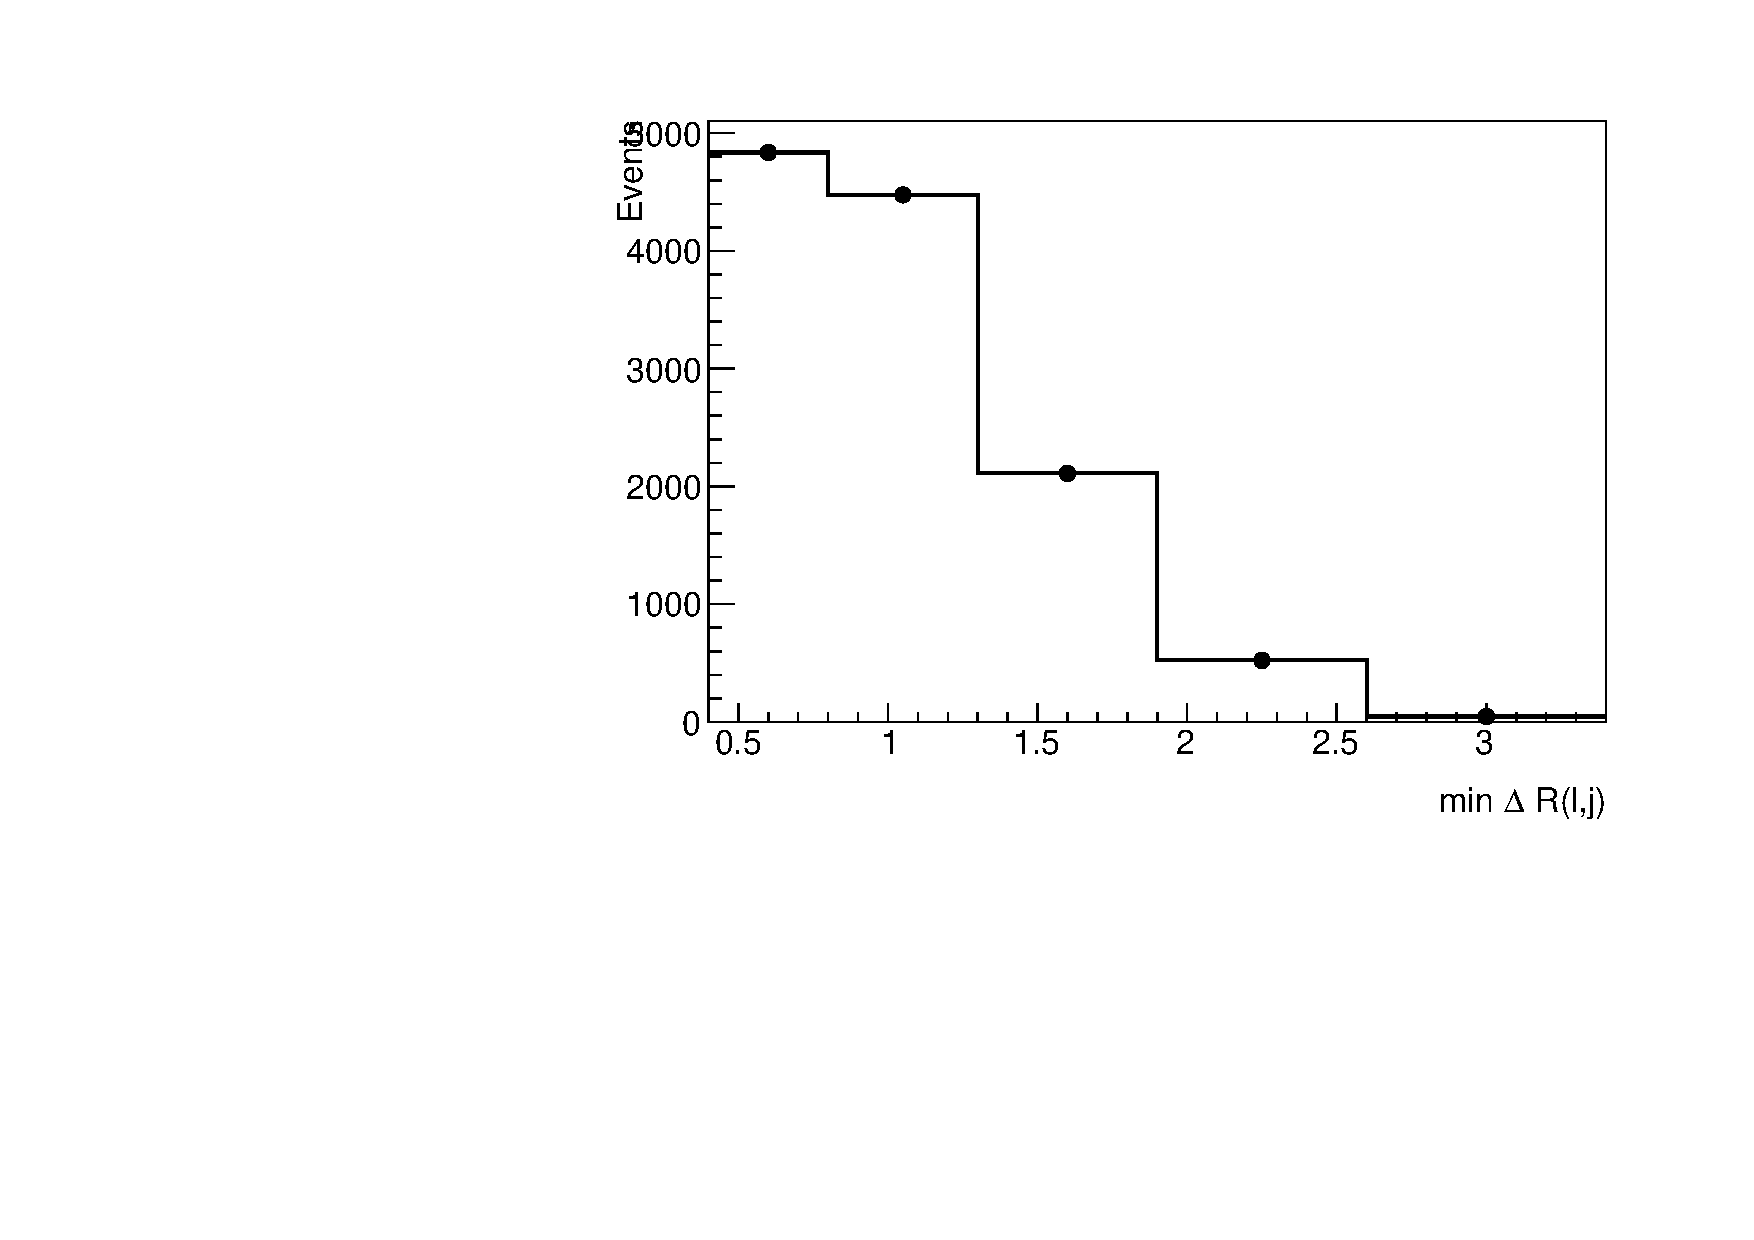
\includegraphics[width=0.4\textwidth]{figures/diff_xsec/dilep/Truth_dist/tty2l_drlj_all_syst_Unfolding_truth_distribution.pdf}}
    \quad \quad
    % pt j1
    \subfloat[]{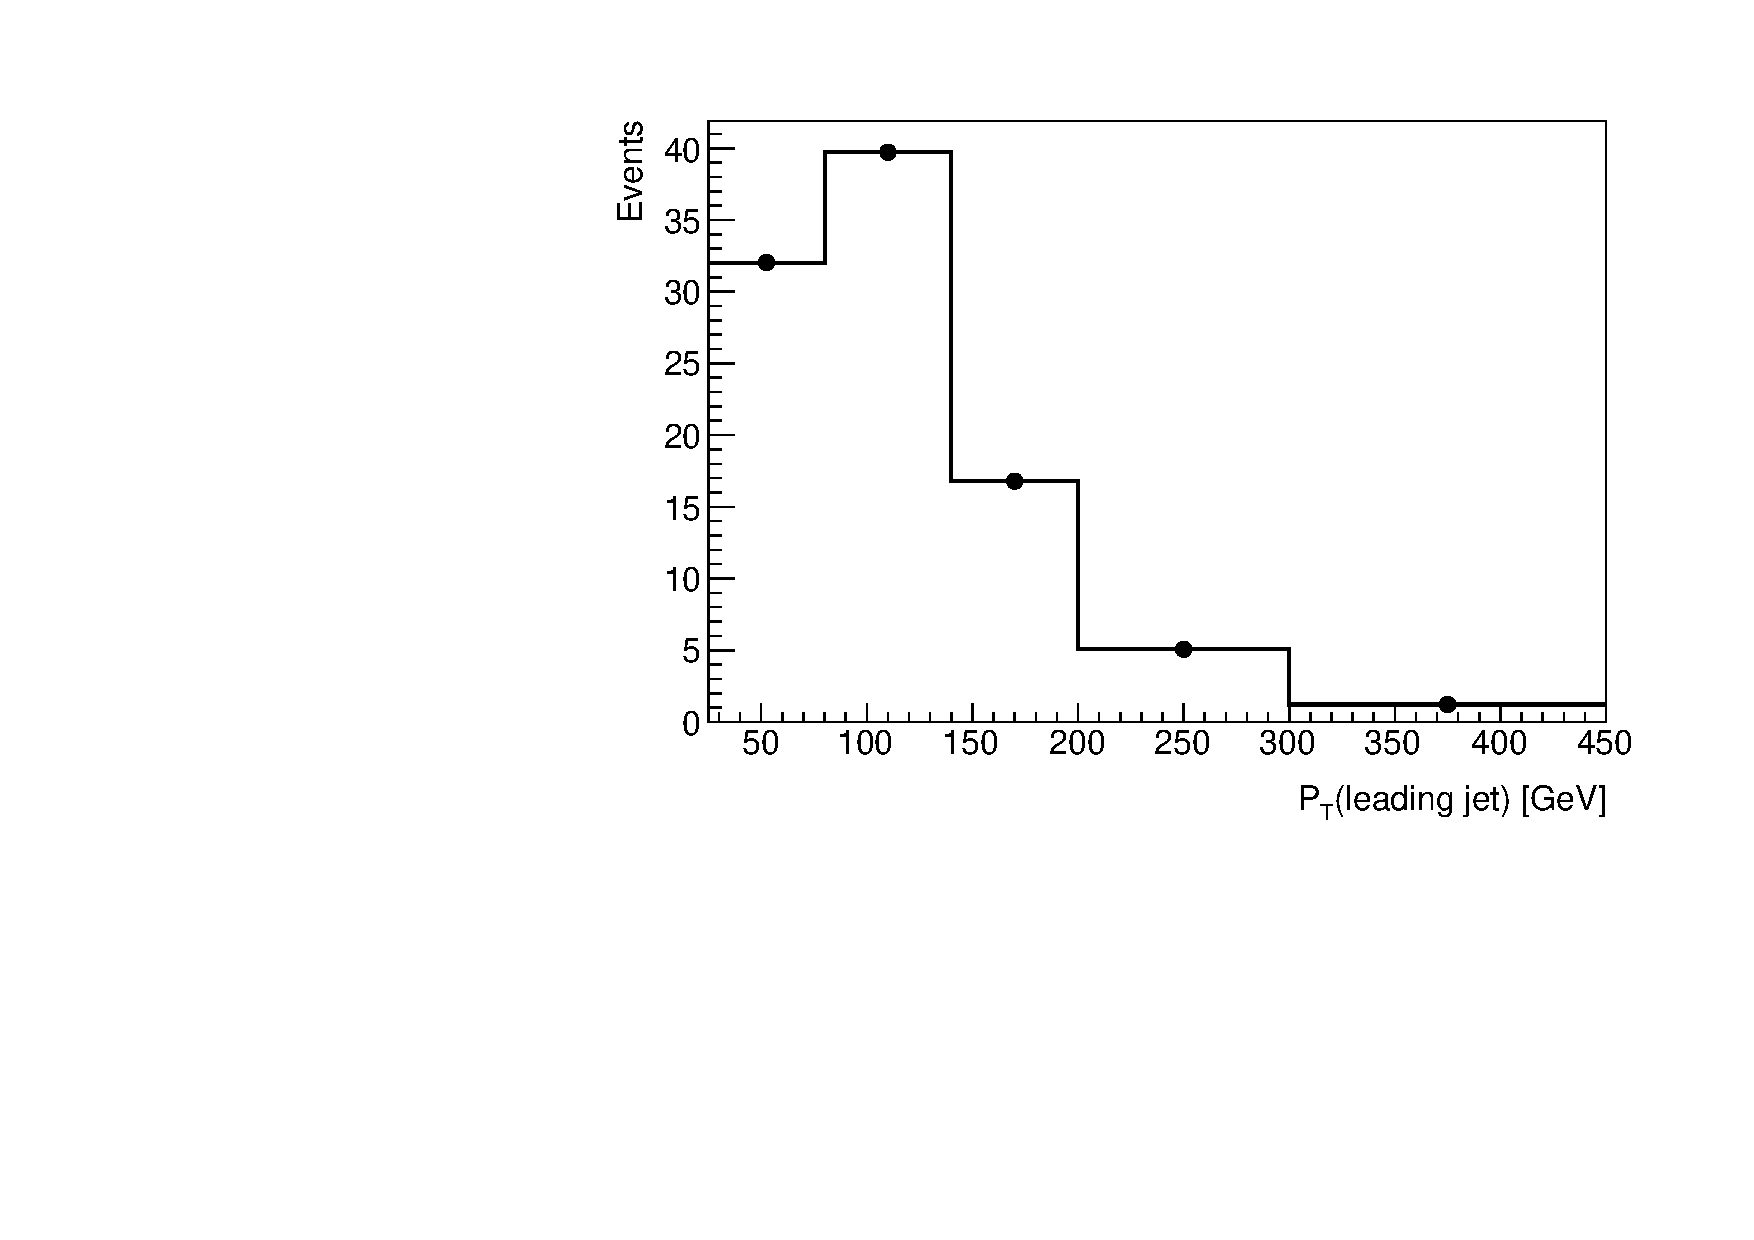
\includegraphics[width=0.4\textwidth]{figures/diff_xsec/dilep/Truth_dist/tty2l_ptj1_all_syst_Unfolding_truth_distribution.pdf}}
    \caption{The particle level distribution of $t\bar{t}\gamma$ (prod) (MC signal) for different observables in the di-lepton channel. Number of events corresponds to the expected number of events at particle level normalised to the luminosity of data. Overflow events are included in the last bin of the corresponding distribution.
    Note that values are divided by bin width.}
    \label{fig:folding_input_dilep2}
\end{figure}
\FloatBarrier


%%%%%%%%
%  Migration matrices ljet 
%%%%%%%%
\begin{figure}[ht]
    \centering
    \subfloat[]{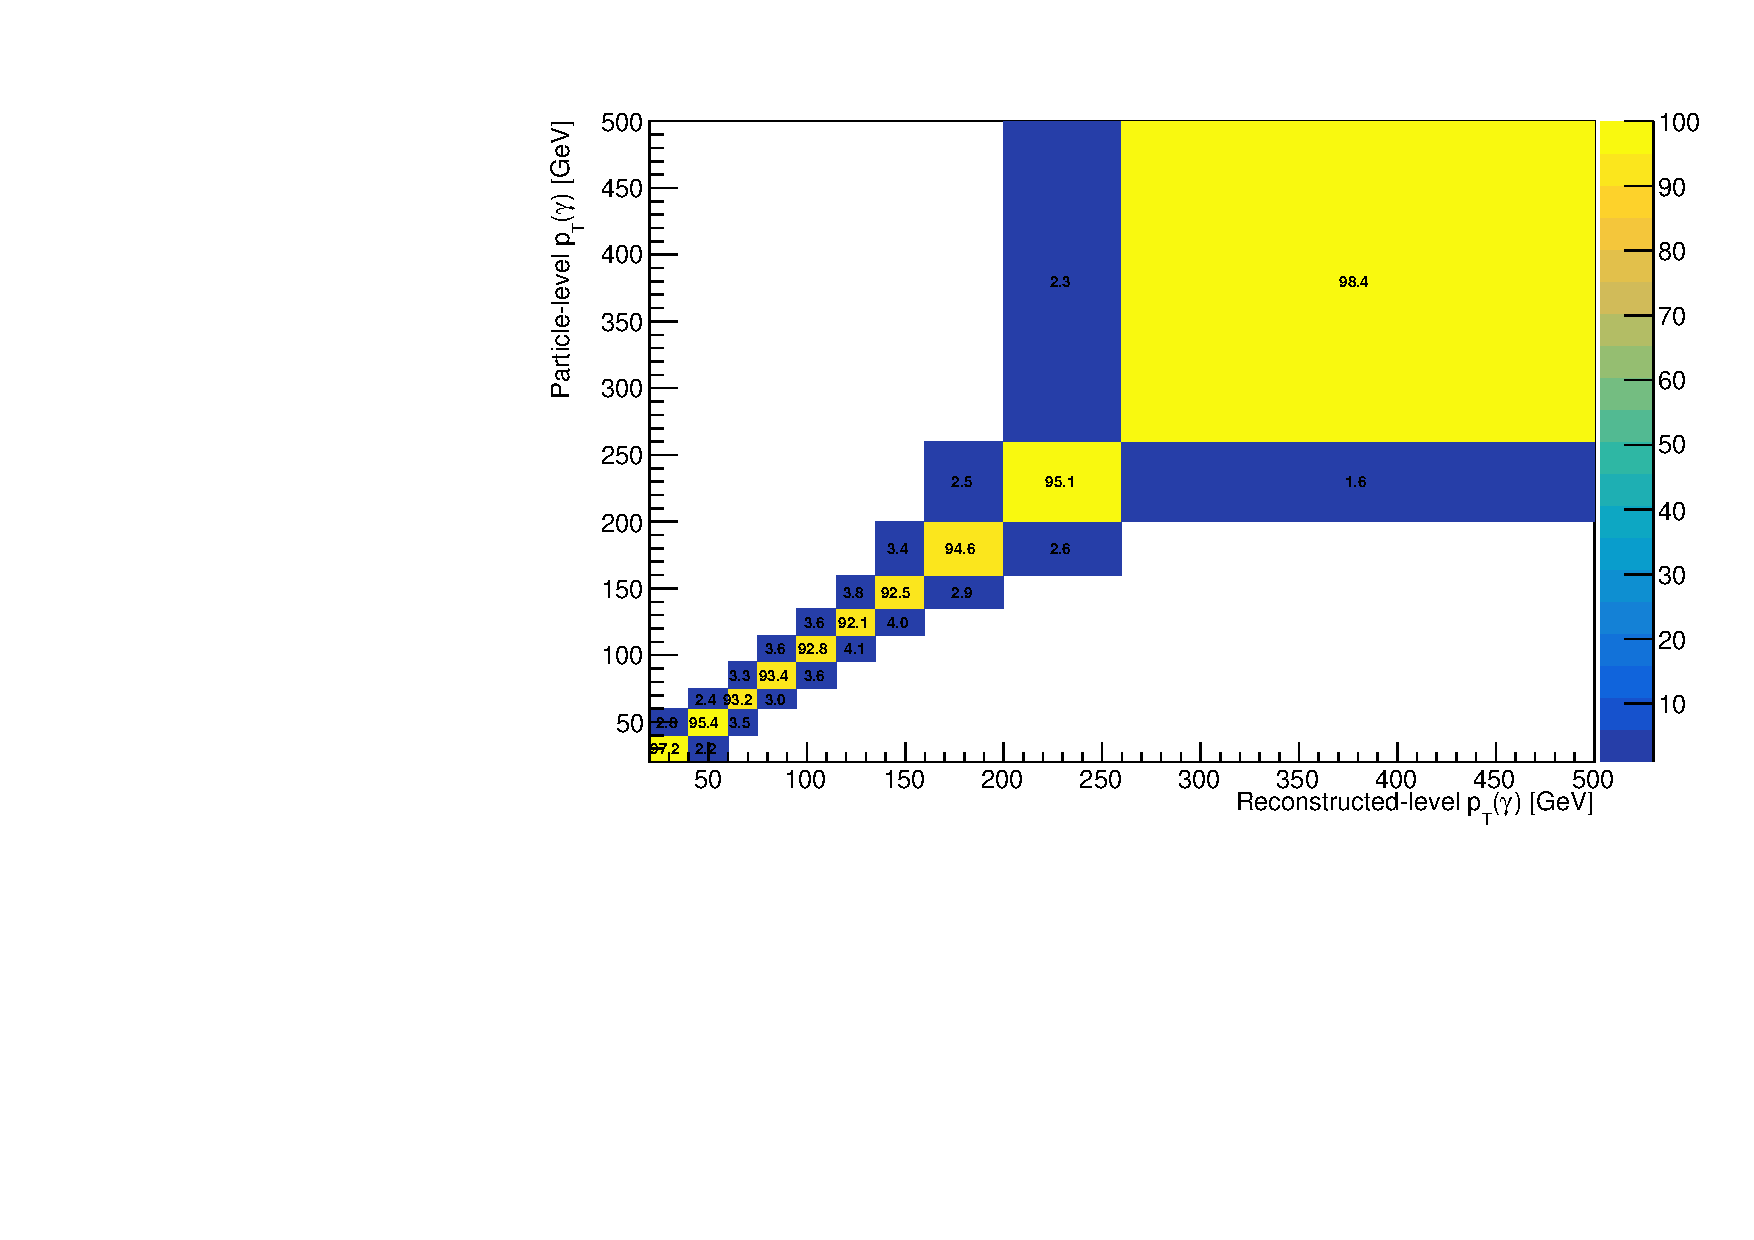
\includegraphics[width=0.4\textwidth]{figures/diff_xsec/ljet/Migration/migration_h2_ph_pt_reco_part_full_weighted_SR1.pdf}}
    \quad\quad
    \subfloat[]{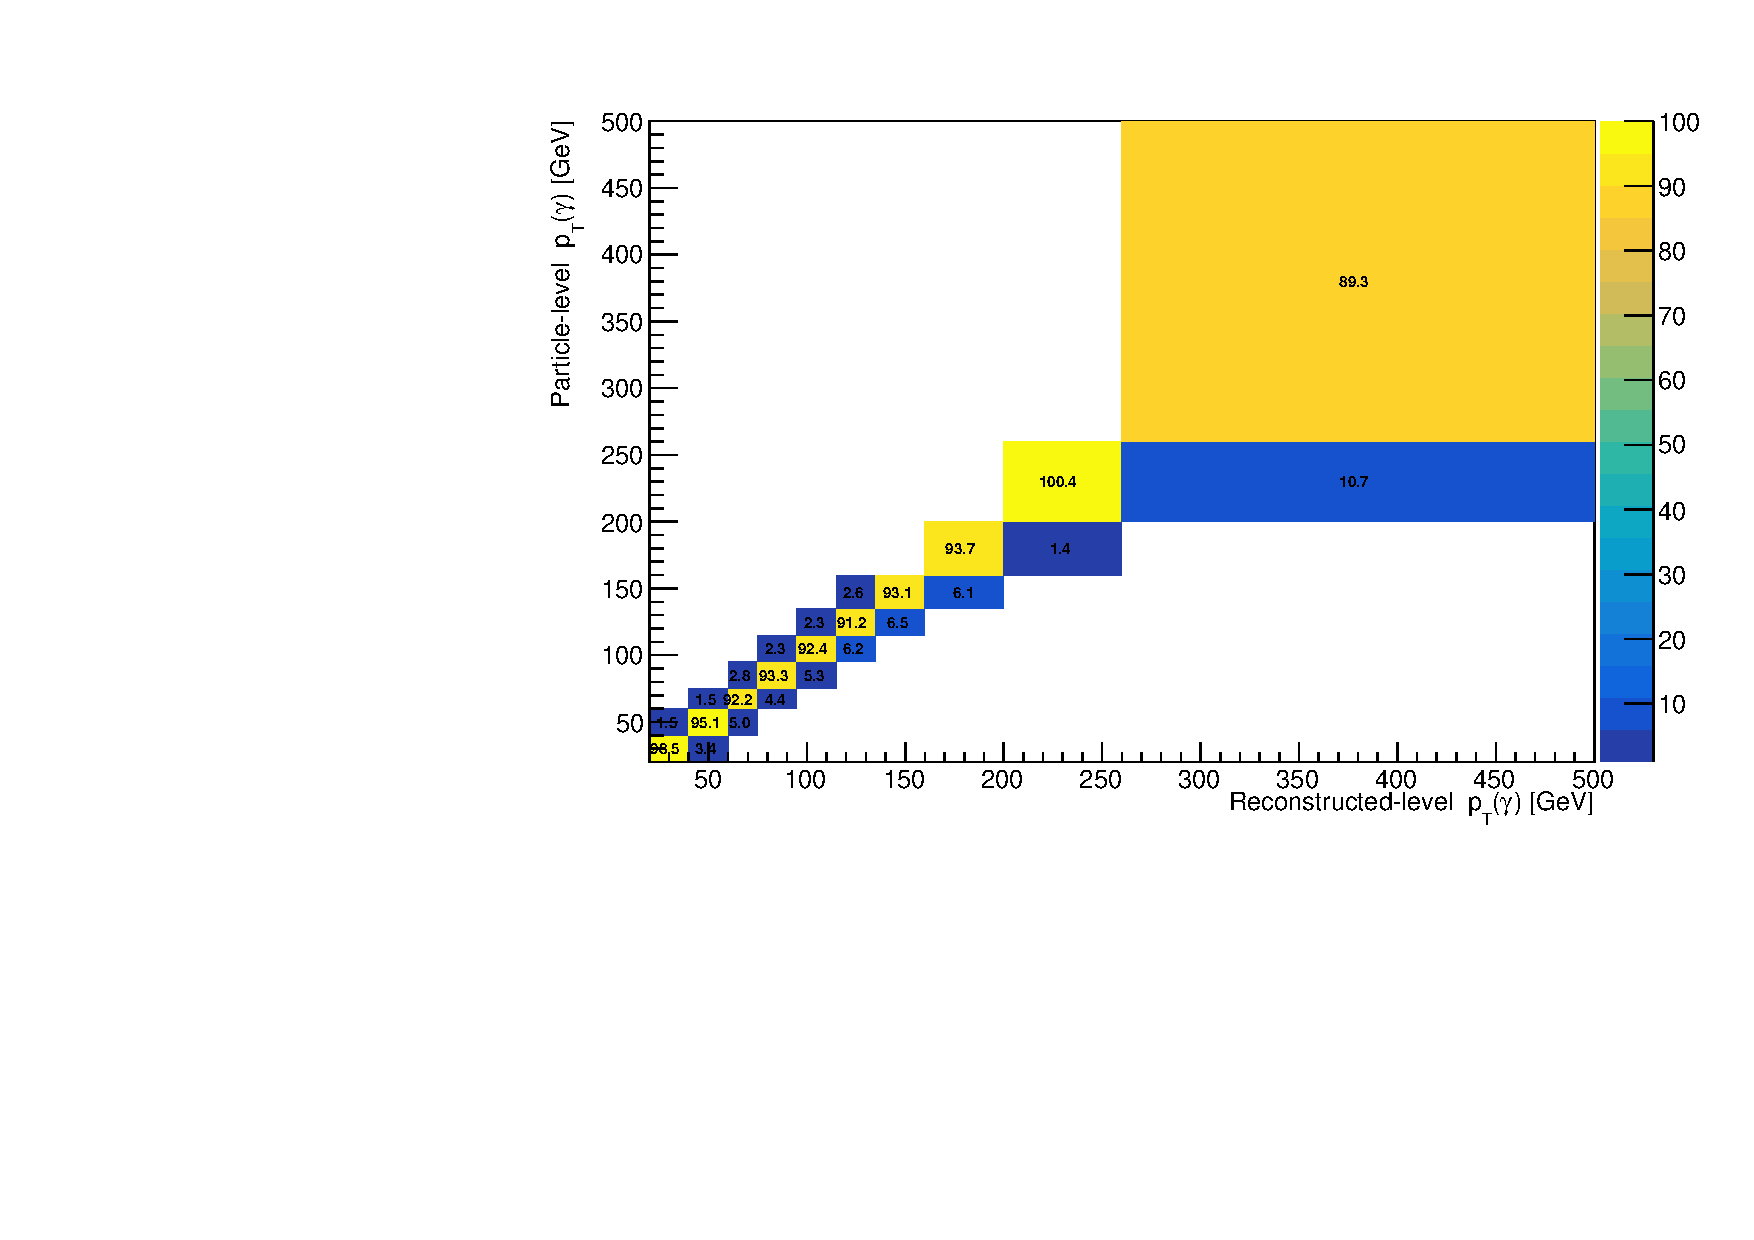
\includegraphics[width=0.4\textwidth]{figures/diff_xsec/ljet/Migration/migration_h2_ph_pt_reco_part_full_weighted_SR2.pdf}}
    \quad\quad
    \subfloat[]{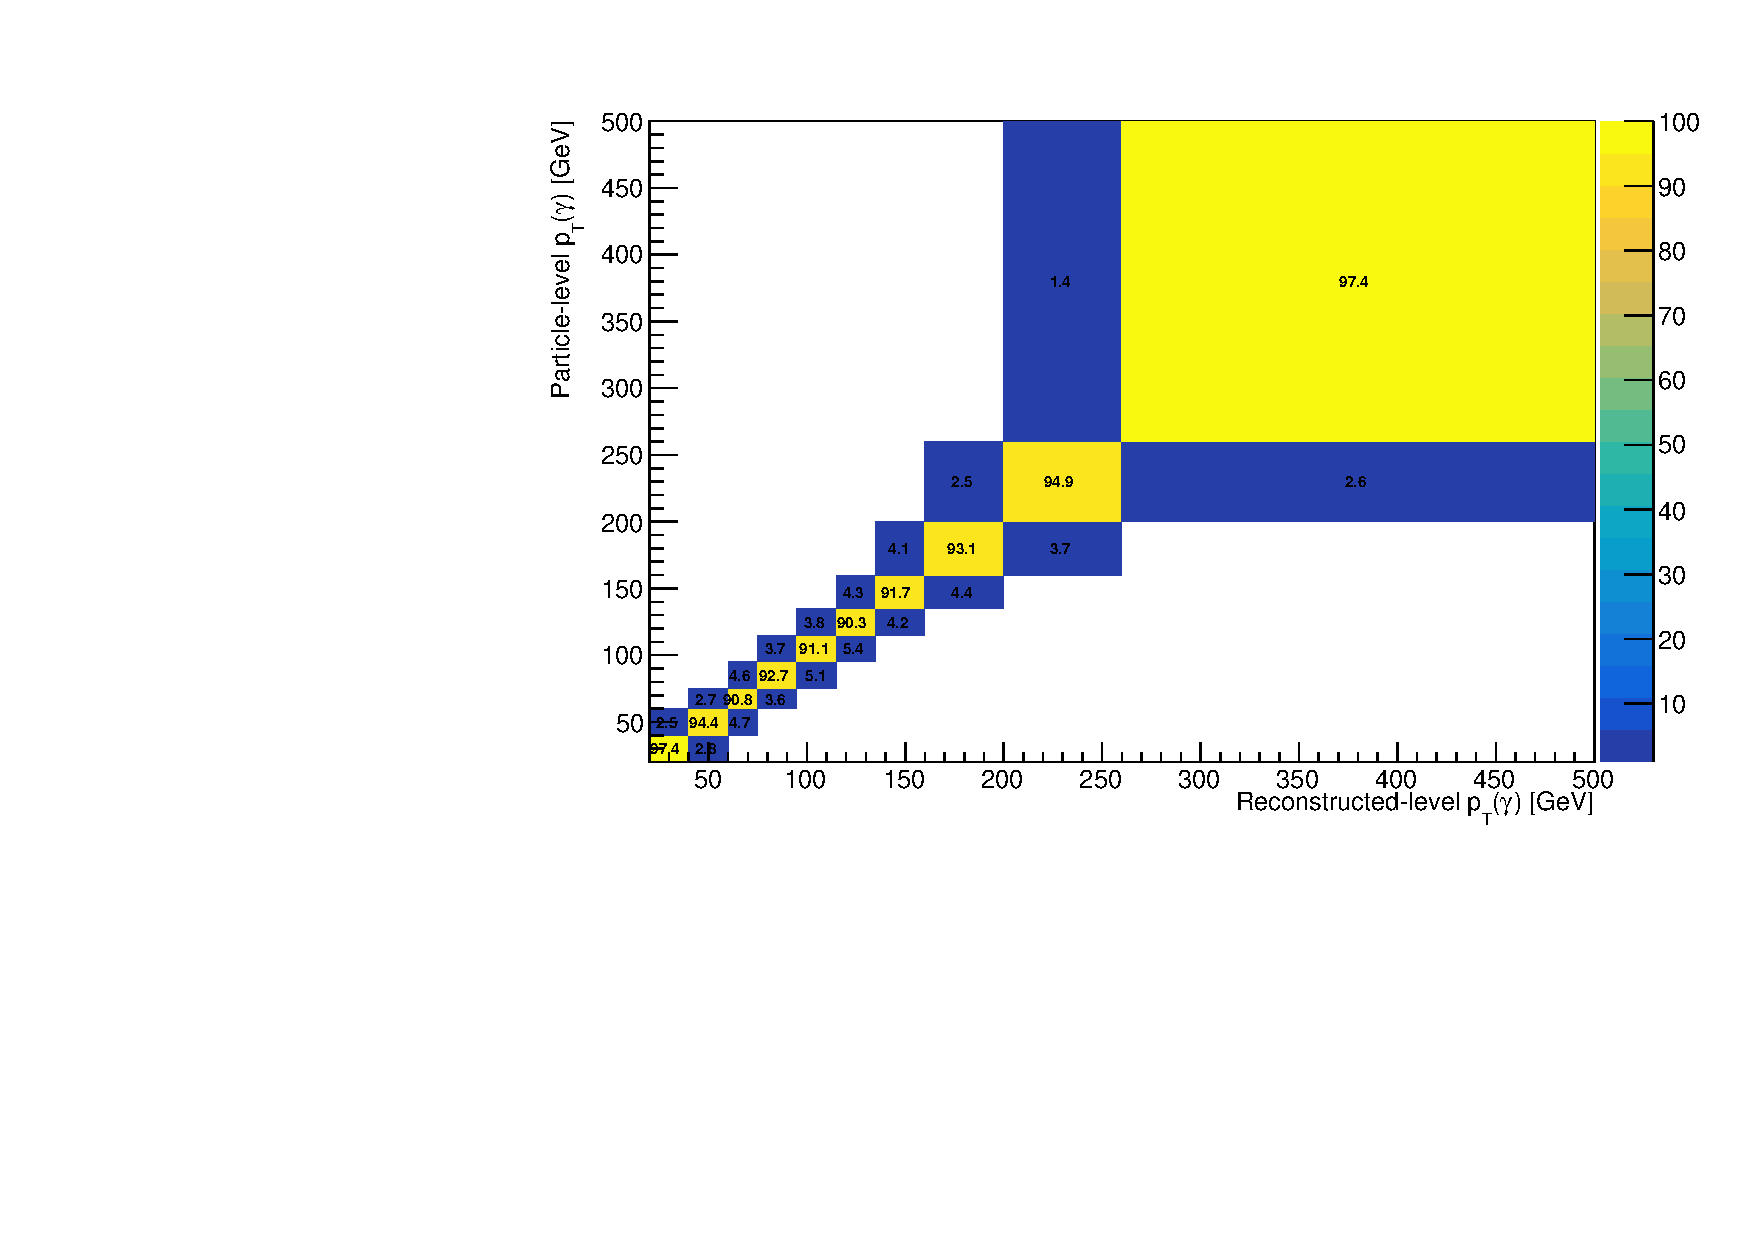
\includegraphics[width=0.4\textwidth]{figures/diff_xsec/ljet/Migration/migration_h2_ph_pt_reco_part_full_weighted_SR3.pdf}}
    \quad\quad
    \subfloat[]{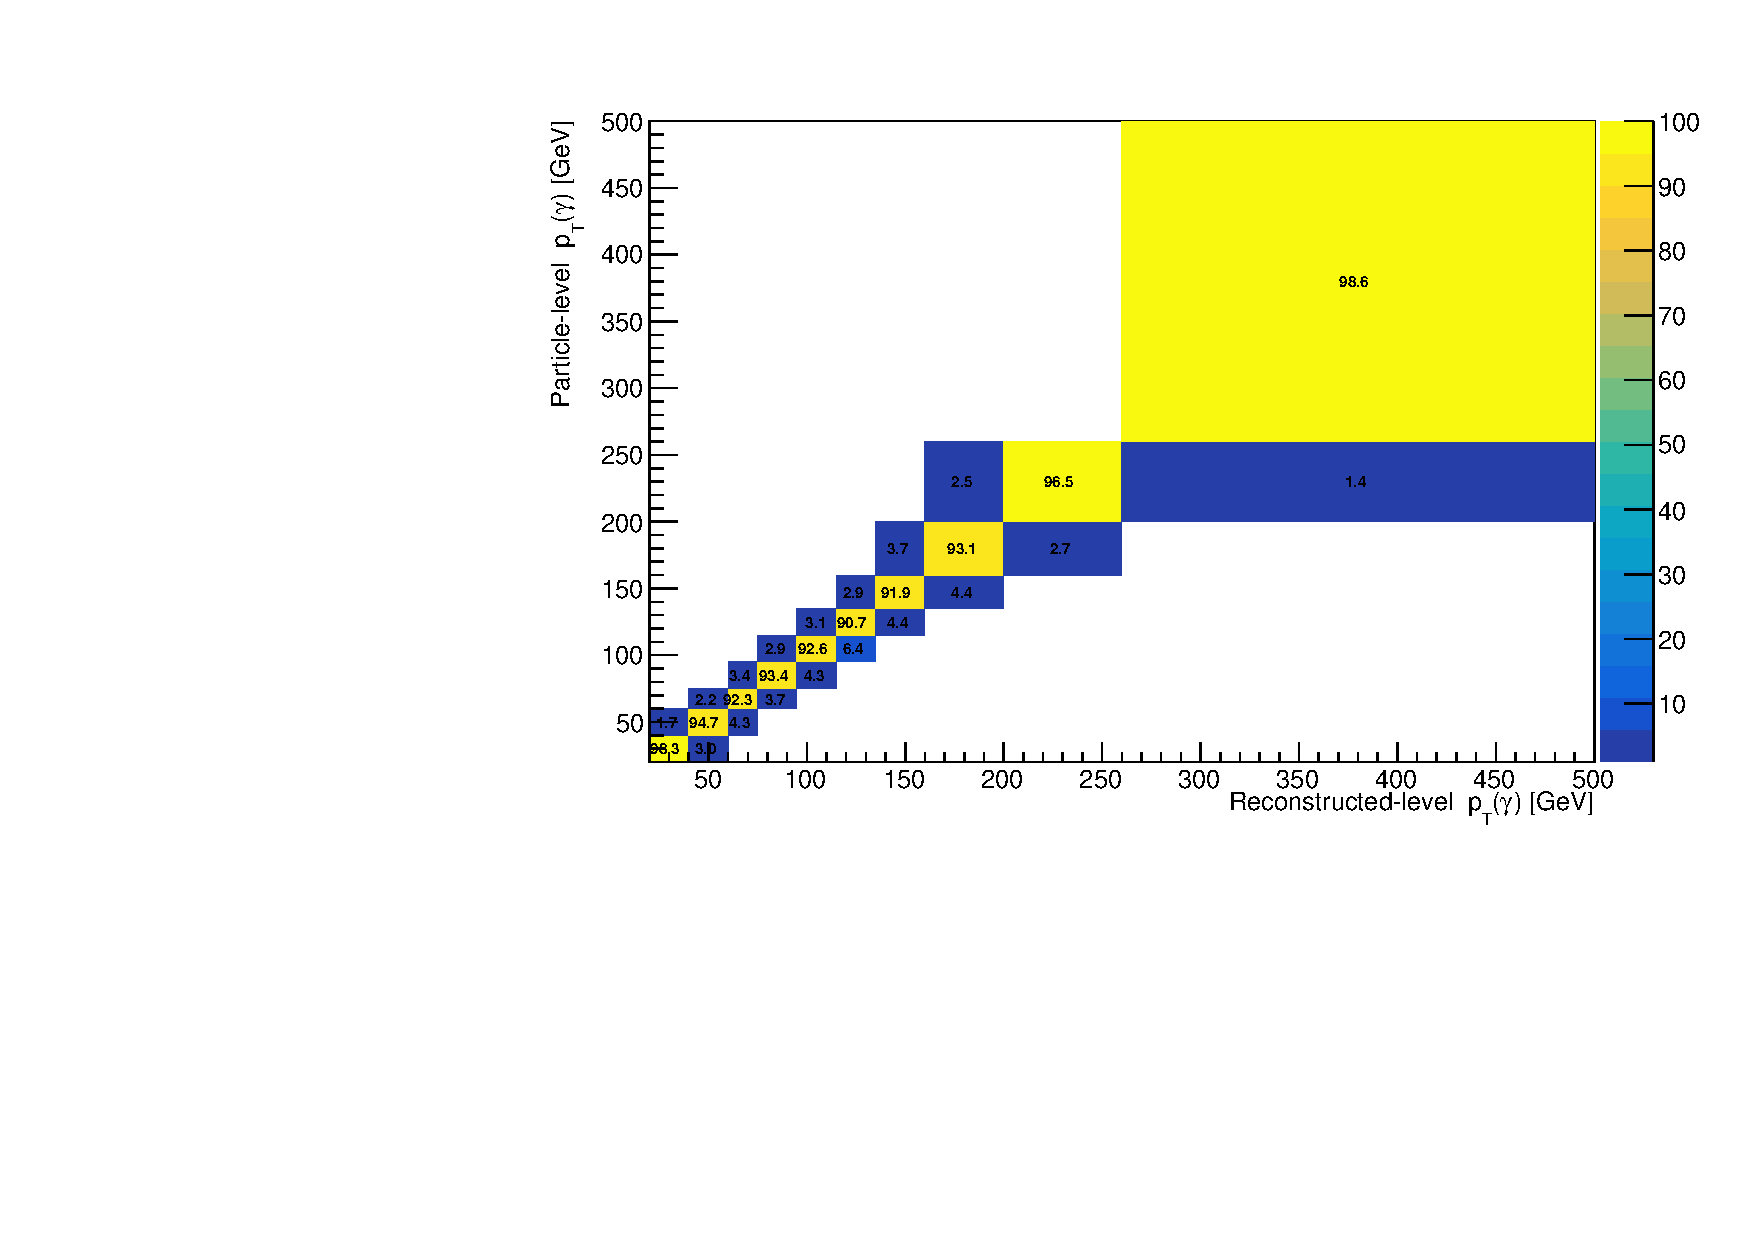
\includegraphics[width=0.4\textwidth]{figures/diff_xsec/ljet/Migration/migration_h2_ph_pt_reco_part_full_weighted_SR4.pdf}}
    \quad\quad
    \caption{The normalised migration matrices, $M_{\mathrm{r,t}}$, representing the migration of events from particle level to reconstruction level  for the four regions defined by the NN: (a) \tty (prod.) enriched region, (b) \tty (dec.) enriched region
    (c) fakes enriched region, (d) prompt photon enriched region for the observable $p_T(\gamma)$ in single lepton channel.}
    \label{fig:folding_input_migration_ljet}
\end{figure}
\FloatBarrier

%%%%%%%%
%  Response matrices ljet
%%%
\begin{figure}[!ht]
  \centering
  \subfloat[]{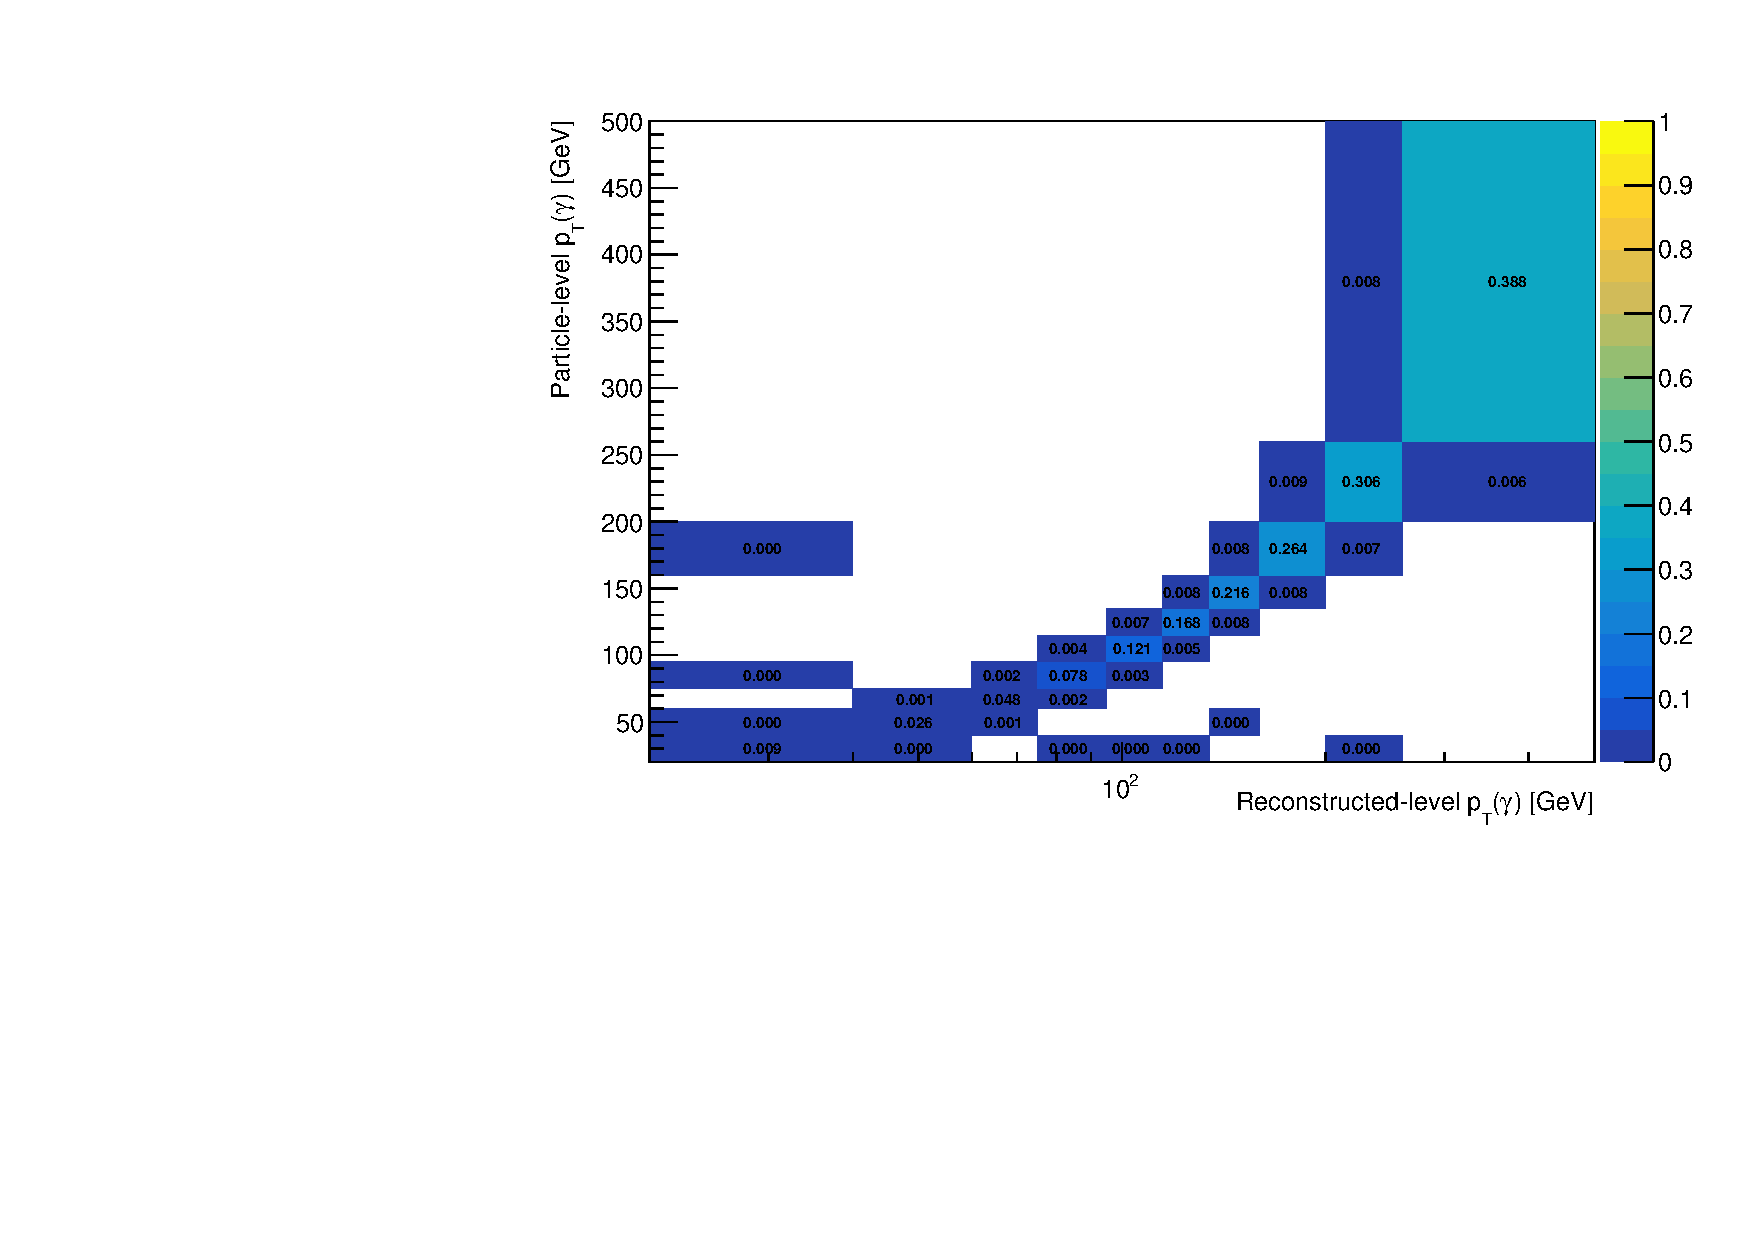
\includegraphics[width=0.4\textwidth]{figures/diff_xsec/ljet/Migration/response_h2_response_matrix_ph_pt_SR1.pdf}}
  \quad\quad
  \subfloat[]{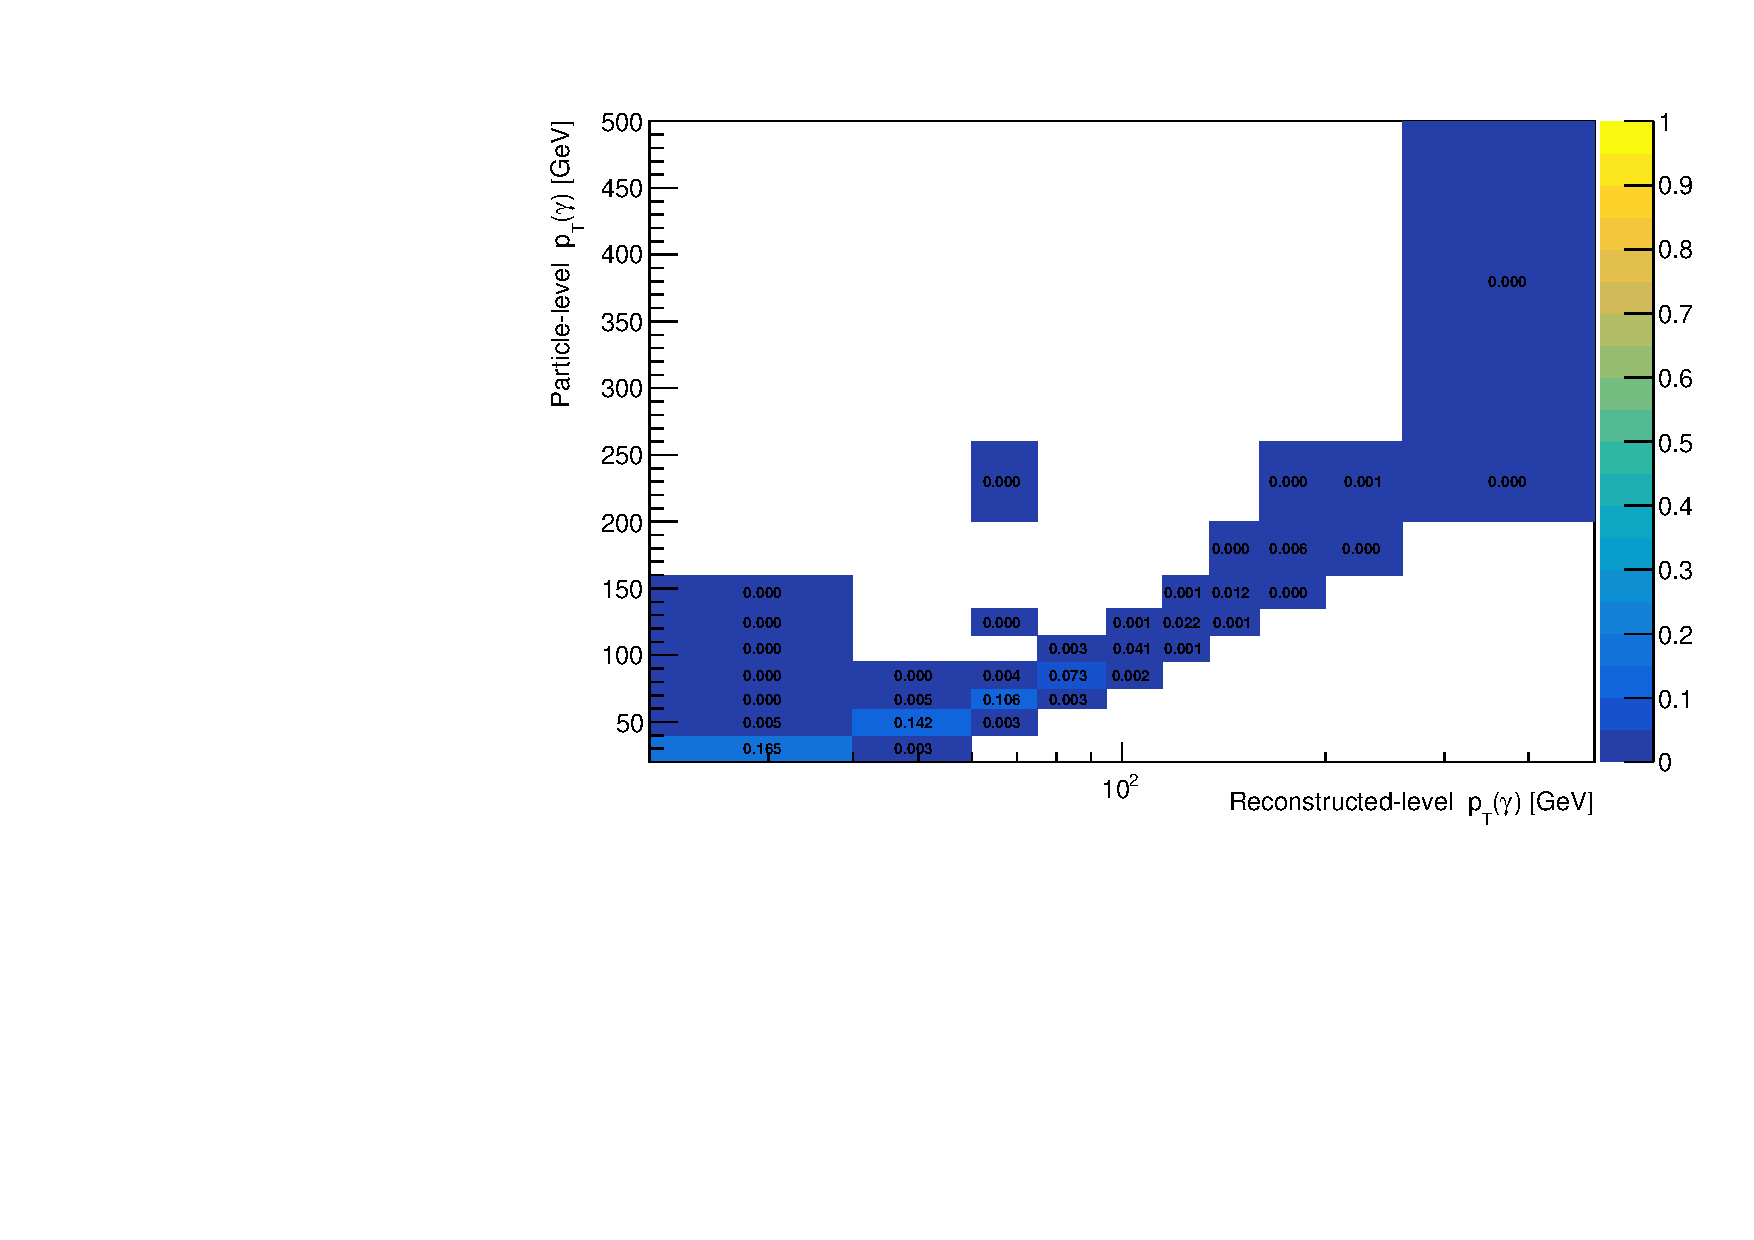
\includegraphics[width=0.4\textwidth]{figures/diff_xsec/ljet/Migration/response_h2_response_matrix_ph_pt_SR2.pdf}}
  \quad\quad
  \subfloat[]{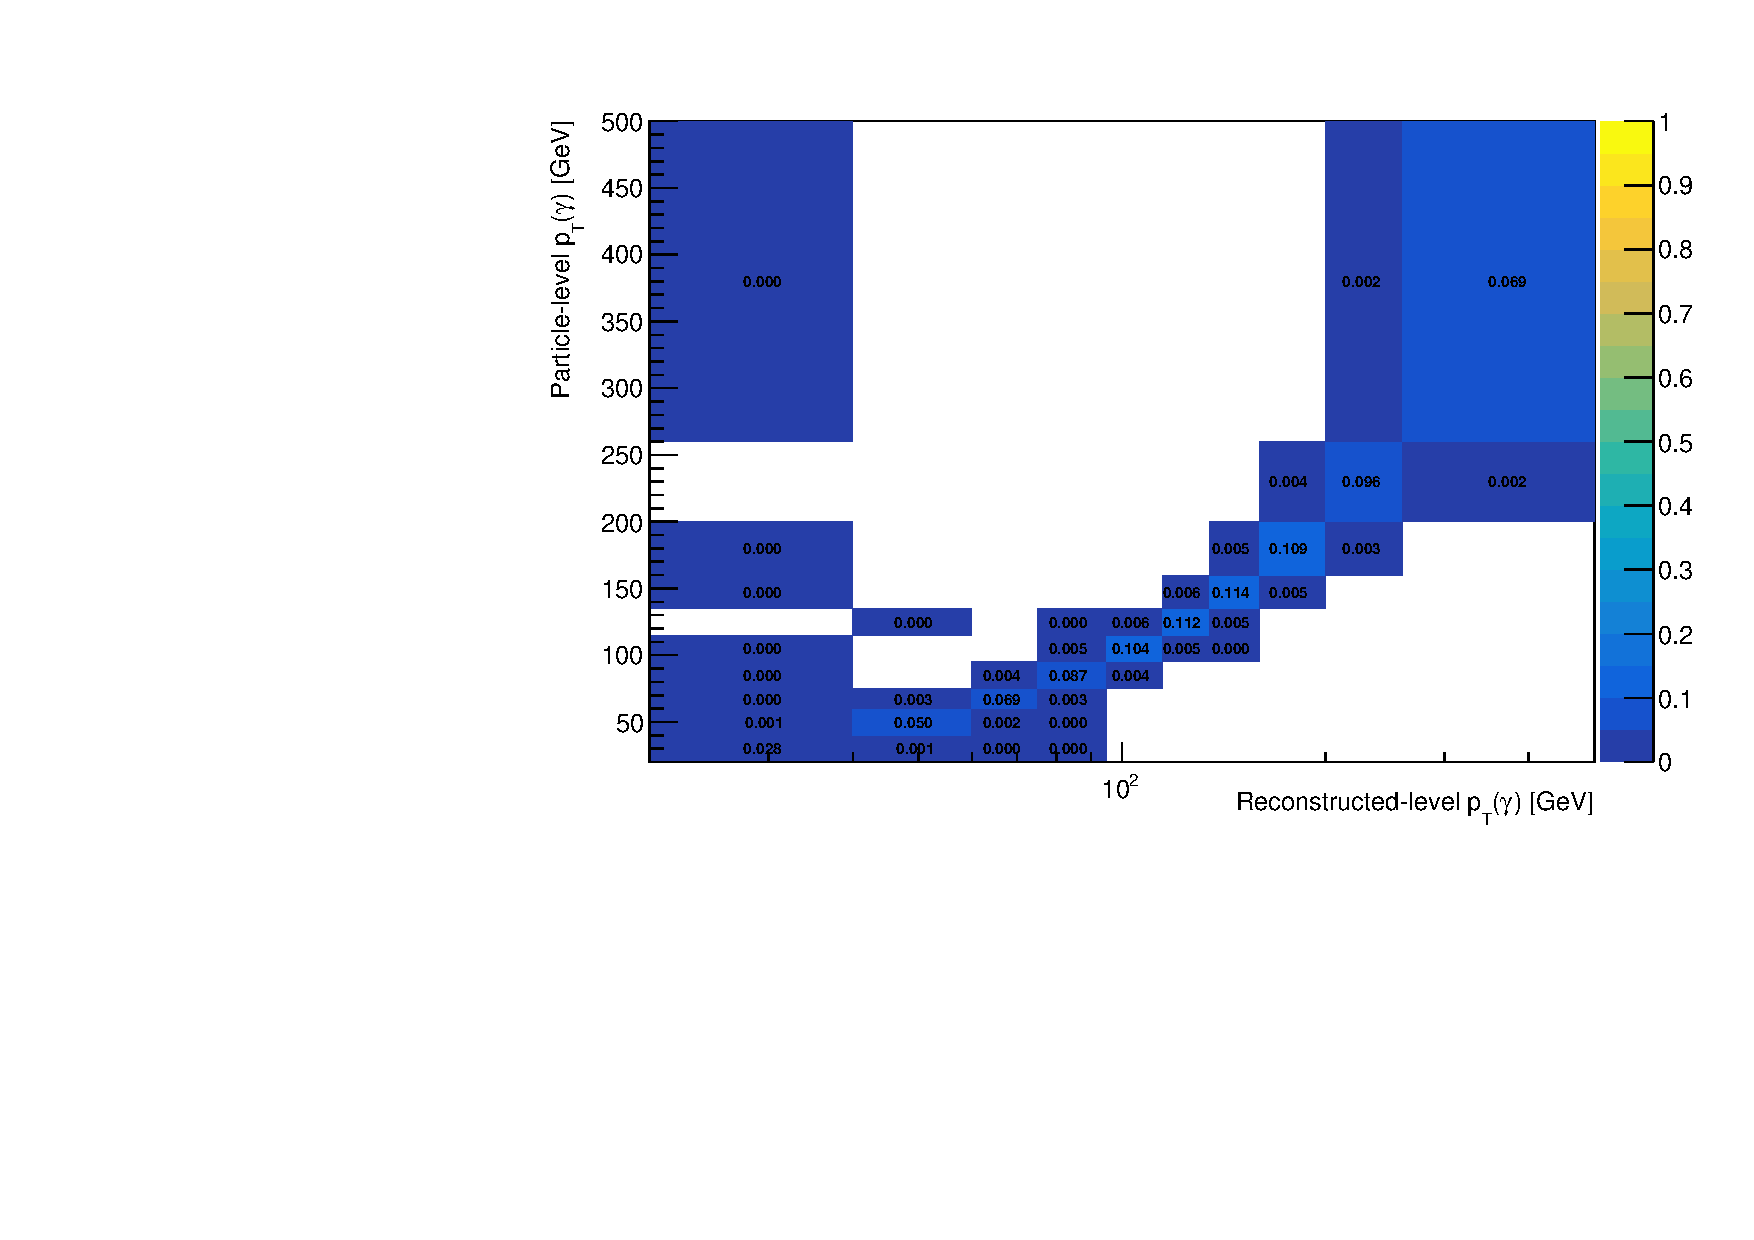
\includegraphics[width=0.4\textwidth]{figures/diff_xsec/ljet/Migration/response_h2_response_matrix_ph_pt_SR3.pdf}}
  \quad\quad
  \subfloat[]{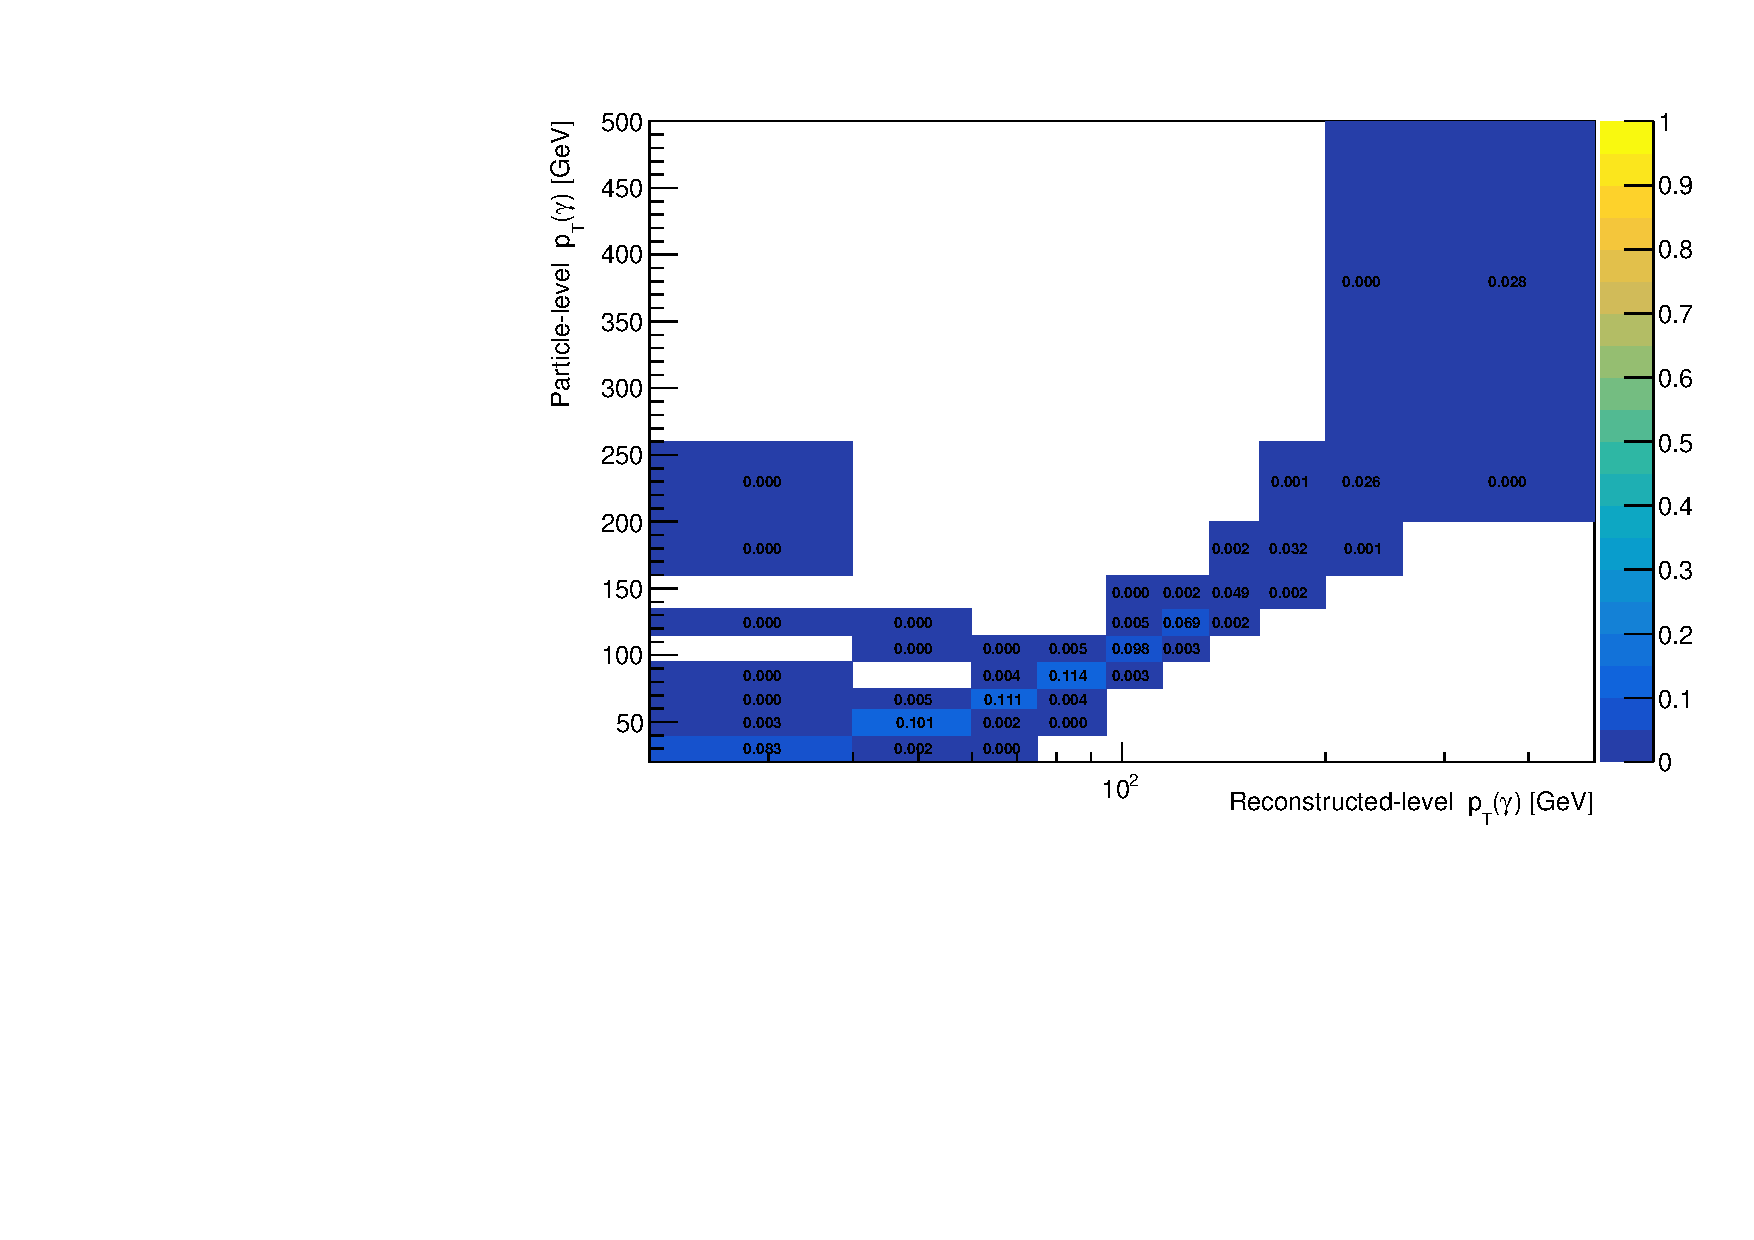
\includegraphics[width=0.4\textwidth]{figures/diff_xsec/ljet/Migration/response_h2_response_matrix_ph_pt_SR4.pdf}}
  \caption[Short caption for LoF]{Response matrices for the observable $p_T(\gamma)$ in the l+jets channel, split across four regions determined by the Neural Network (NN) output. (a-d) Response matrices for the \tty (prod.), \tty (dec.), fakes, and prompt photon enriched regions, respectively. -- \emph{Continued on next page}}
  \label{fig:folding_input_response_ljet_pt1}
\end{figure}
\begin{figure}[!ht]
  \ContinuedFloat
  \centering
  \subfloat[]{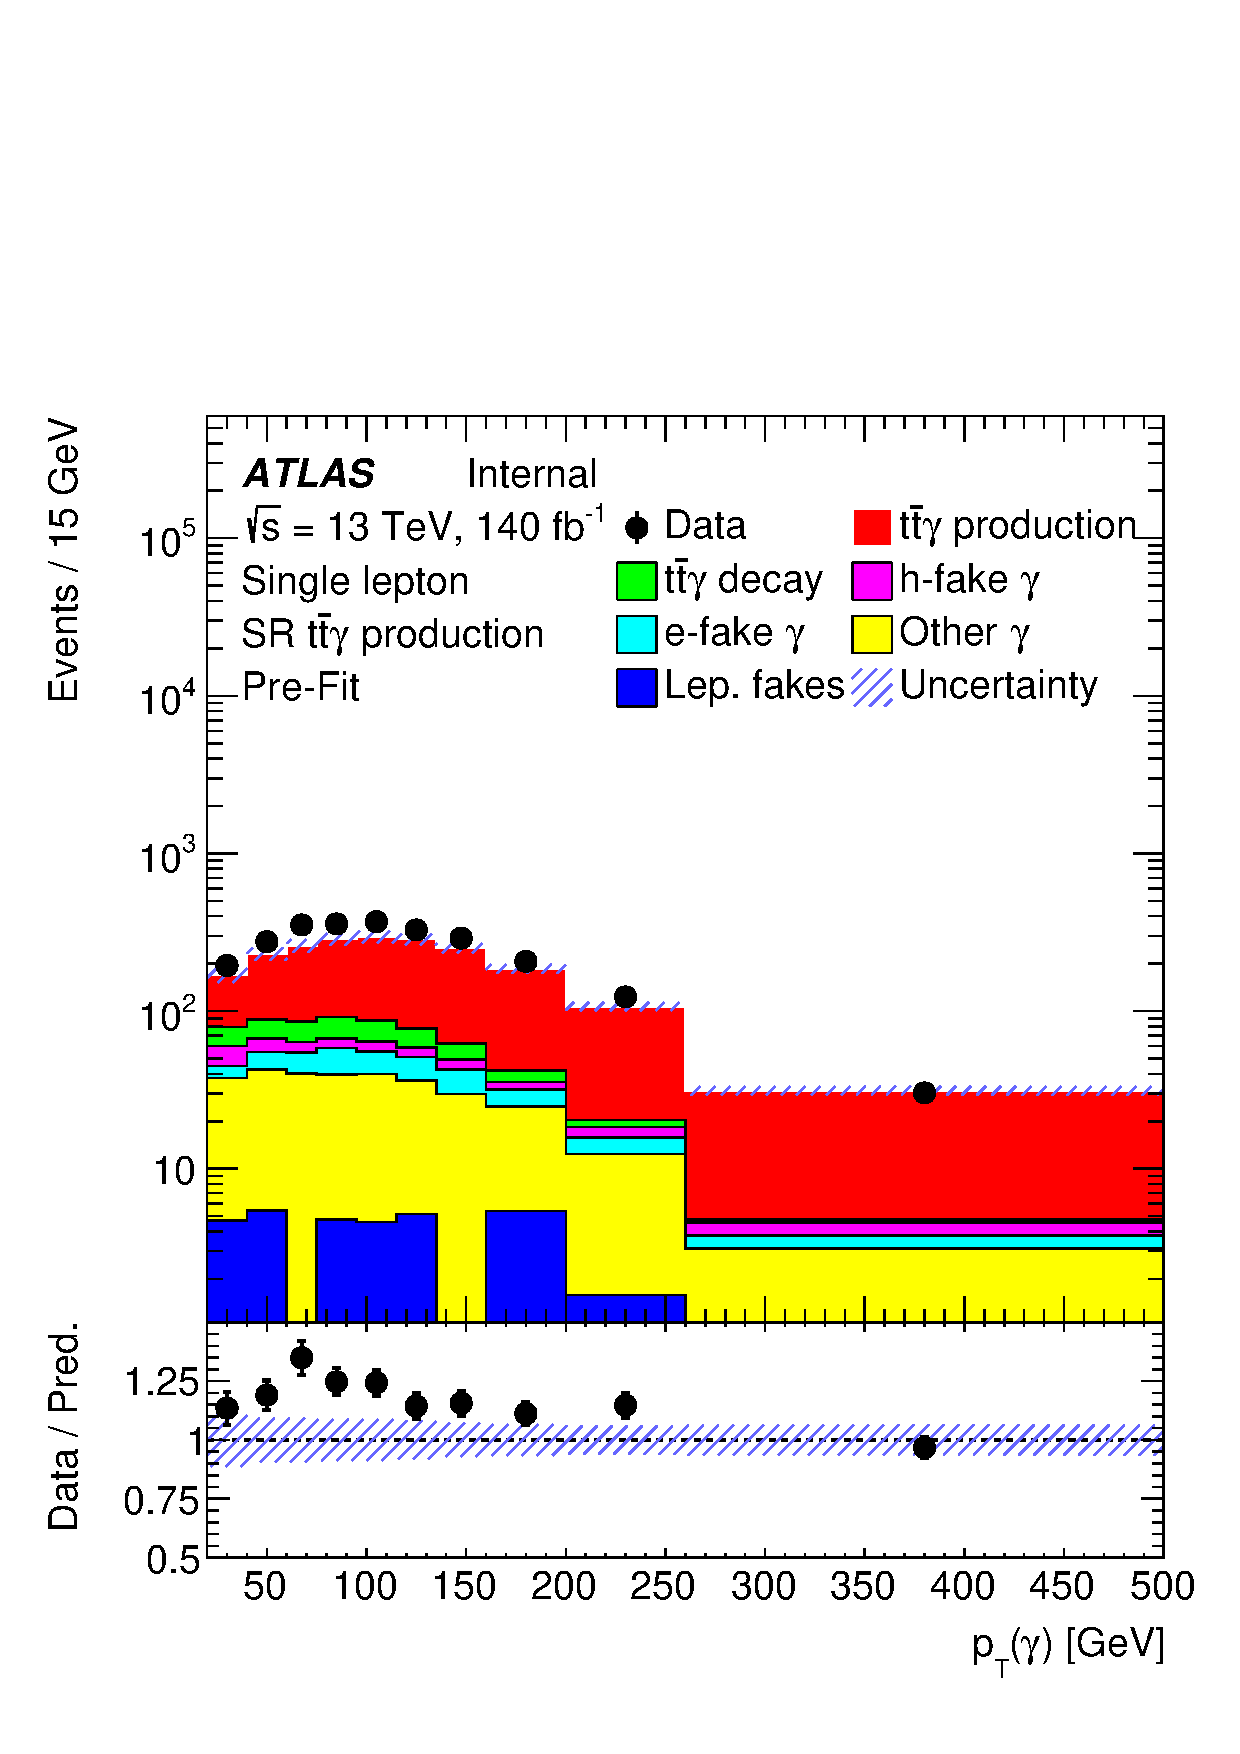
\includegraphics[width=0.4\textwidth]{figures/diff_xsec/ljet/Folded_distributions/tty1l_pt_all_syst/Plots/SR1.pdf}}
  \quad\quad
  \subfloat[]{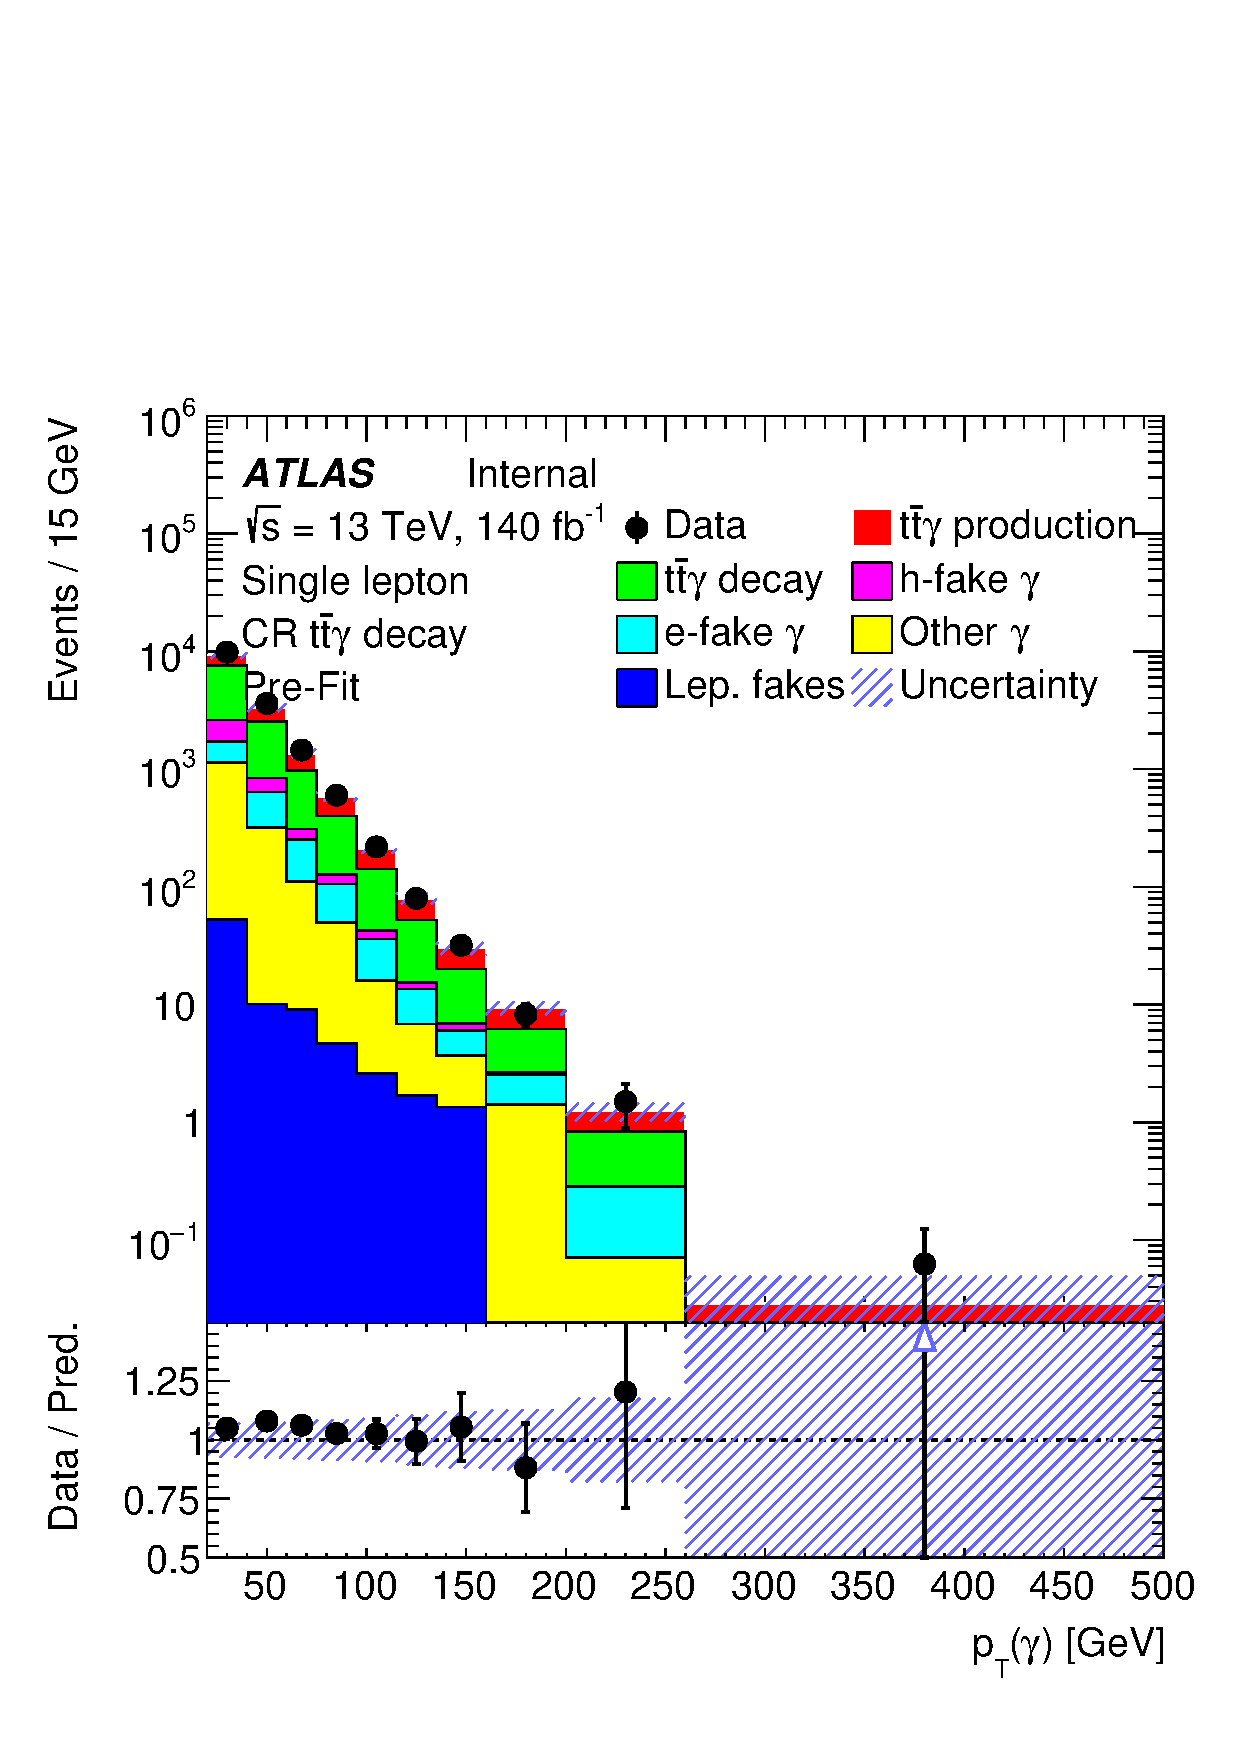
\includegraphics[width=0.4\textwidth]{figures/diff_xsec/ljet/Folded_distributions/tty1l_pt_all_syst/Plots/SR2.pdf}}
  \quad\quad
  \subfloat[]{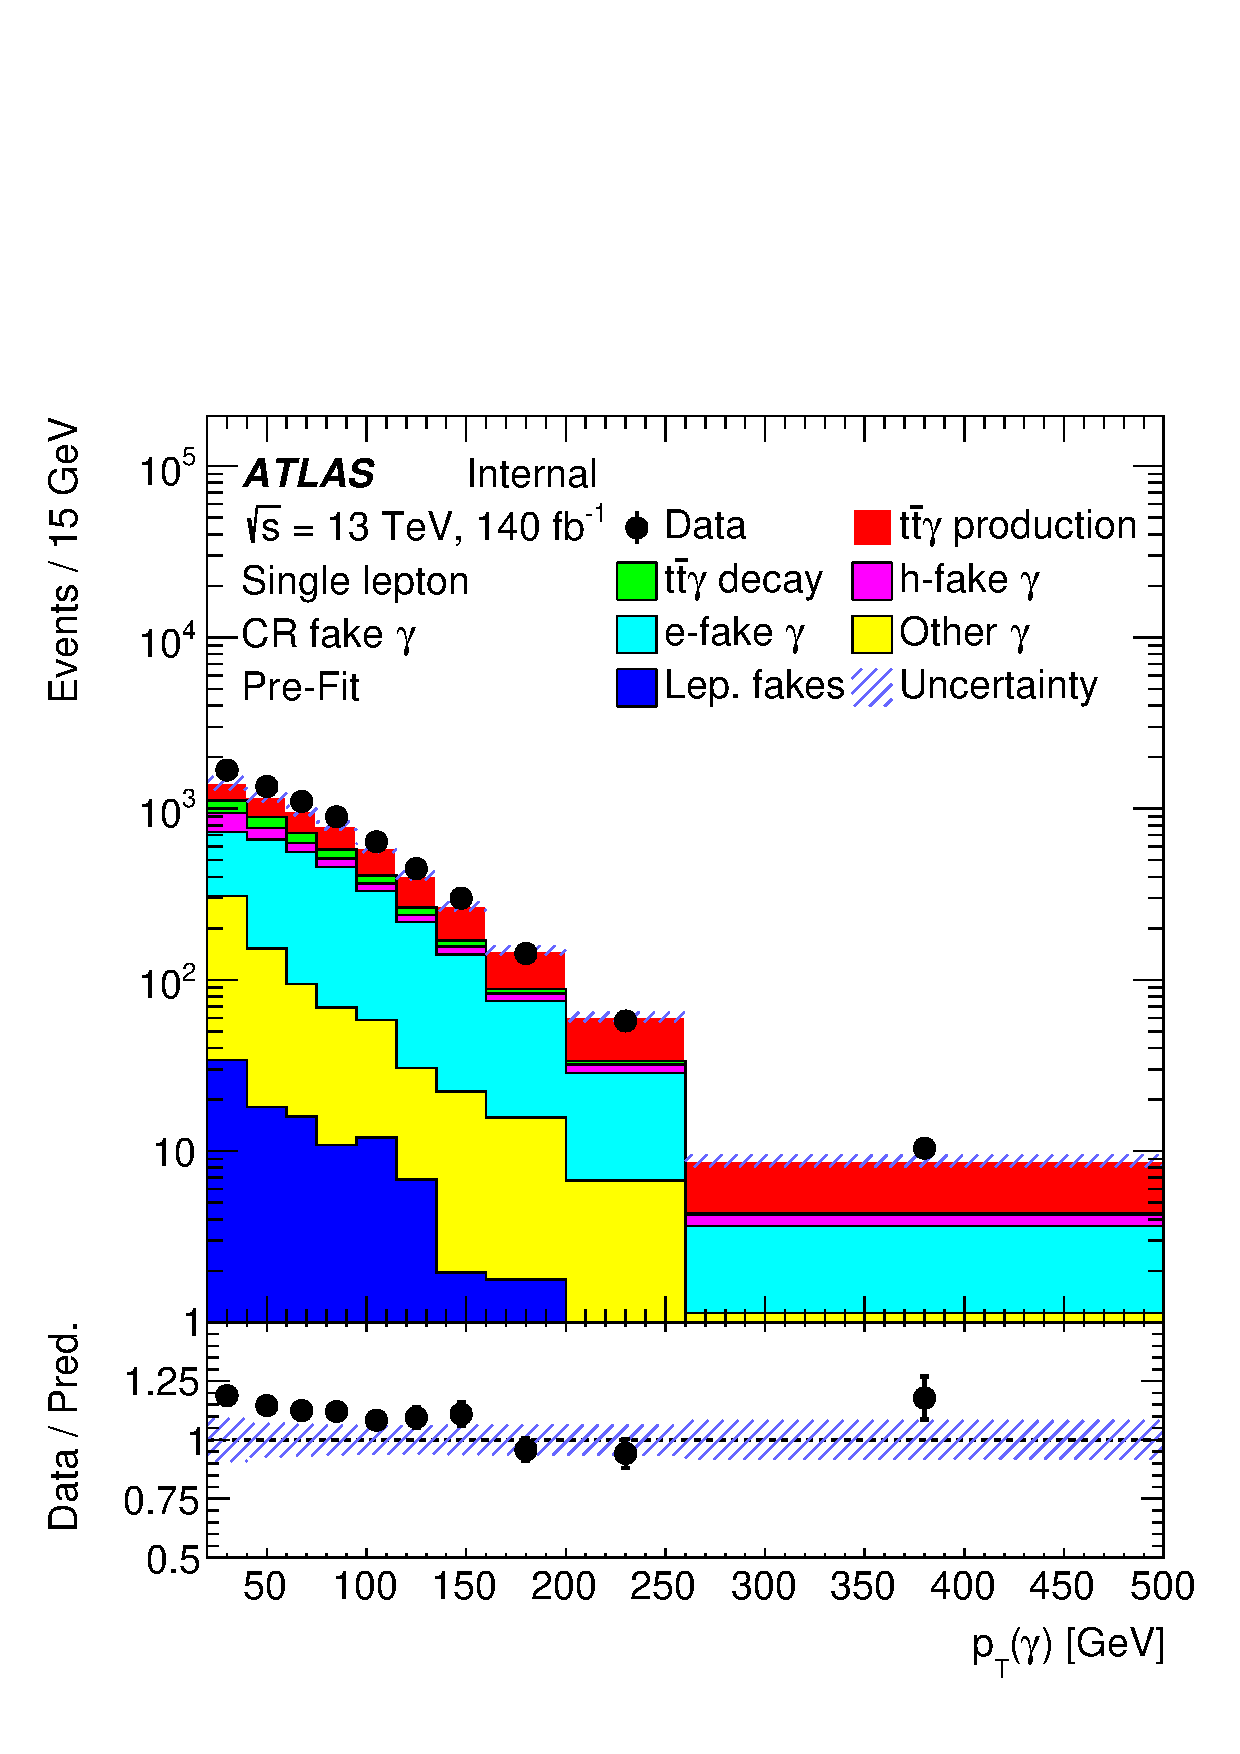
\includegraphics[width=0.4\textwidth]{figures/diff_xsec/ljet/Folded_distributions/tty1l_pt_all_syst/Plots/SR3.pdf}}
  \quad\quad
  \subfloat[]{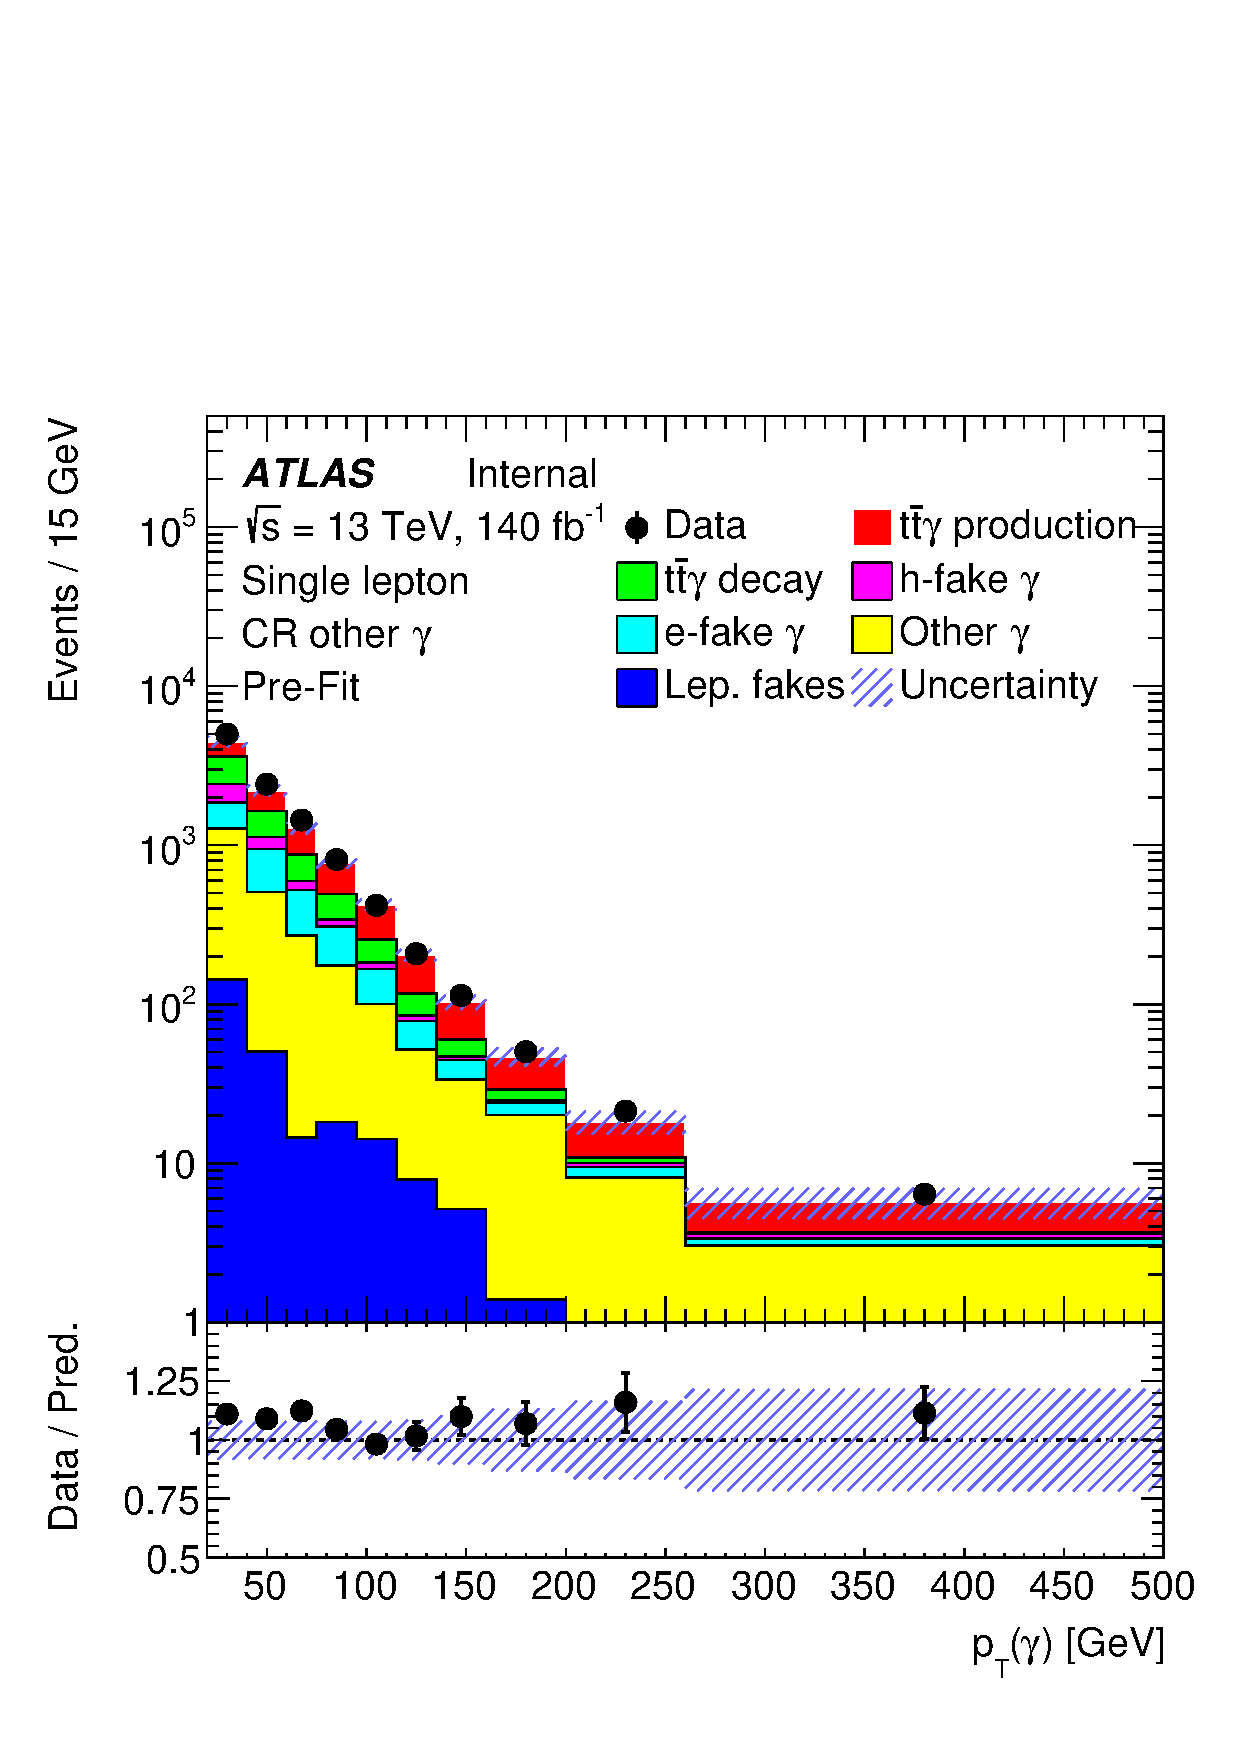
\includegraphics[width=0.4\textwidth]{figures/diff_xsec/ljet/Folded_distributions/tty1l_pt_all_syst/Plots/SR4.pdf}}
  \caption[]{(e-h) Corresponding Data-MC comparisons. The signal distribution at the reconstruction level was created by folding the truth distribution with the respective response matrix.}
  \label{fig:folding_input_response_ljet_pt2}
\end{figure}

%%%%%%%%
%  Migration matrices dilep
%%%%%%%%
\begin{figure}[ht]
    \centering
    \subfloat[]{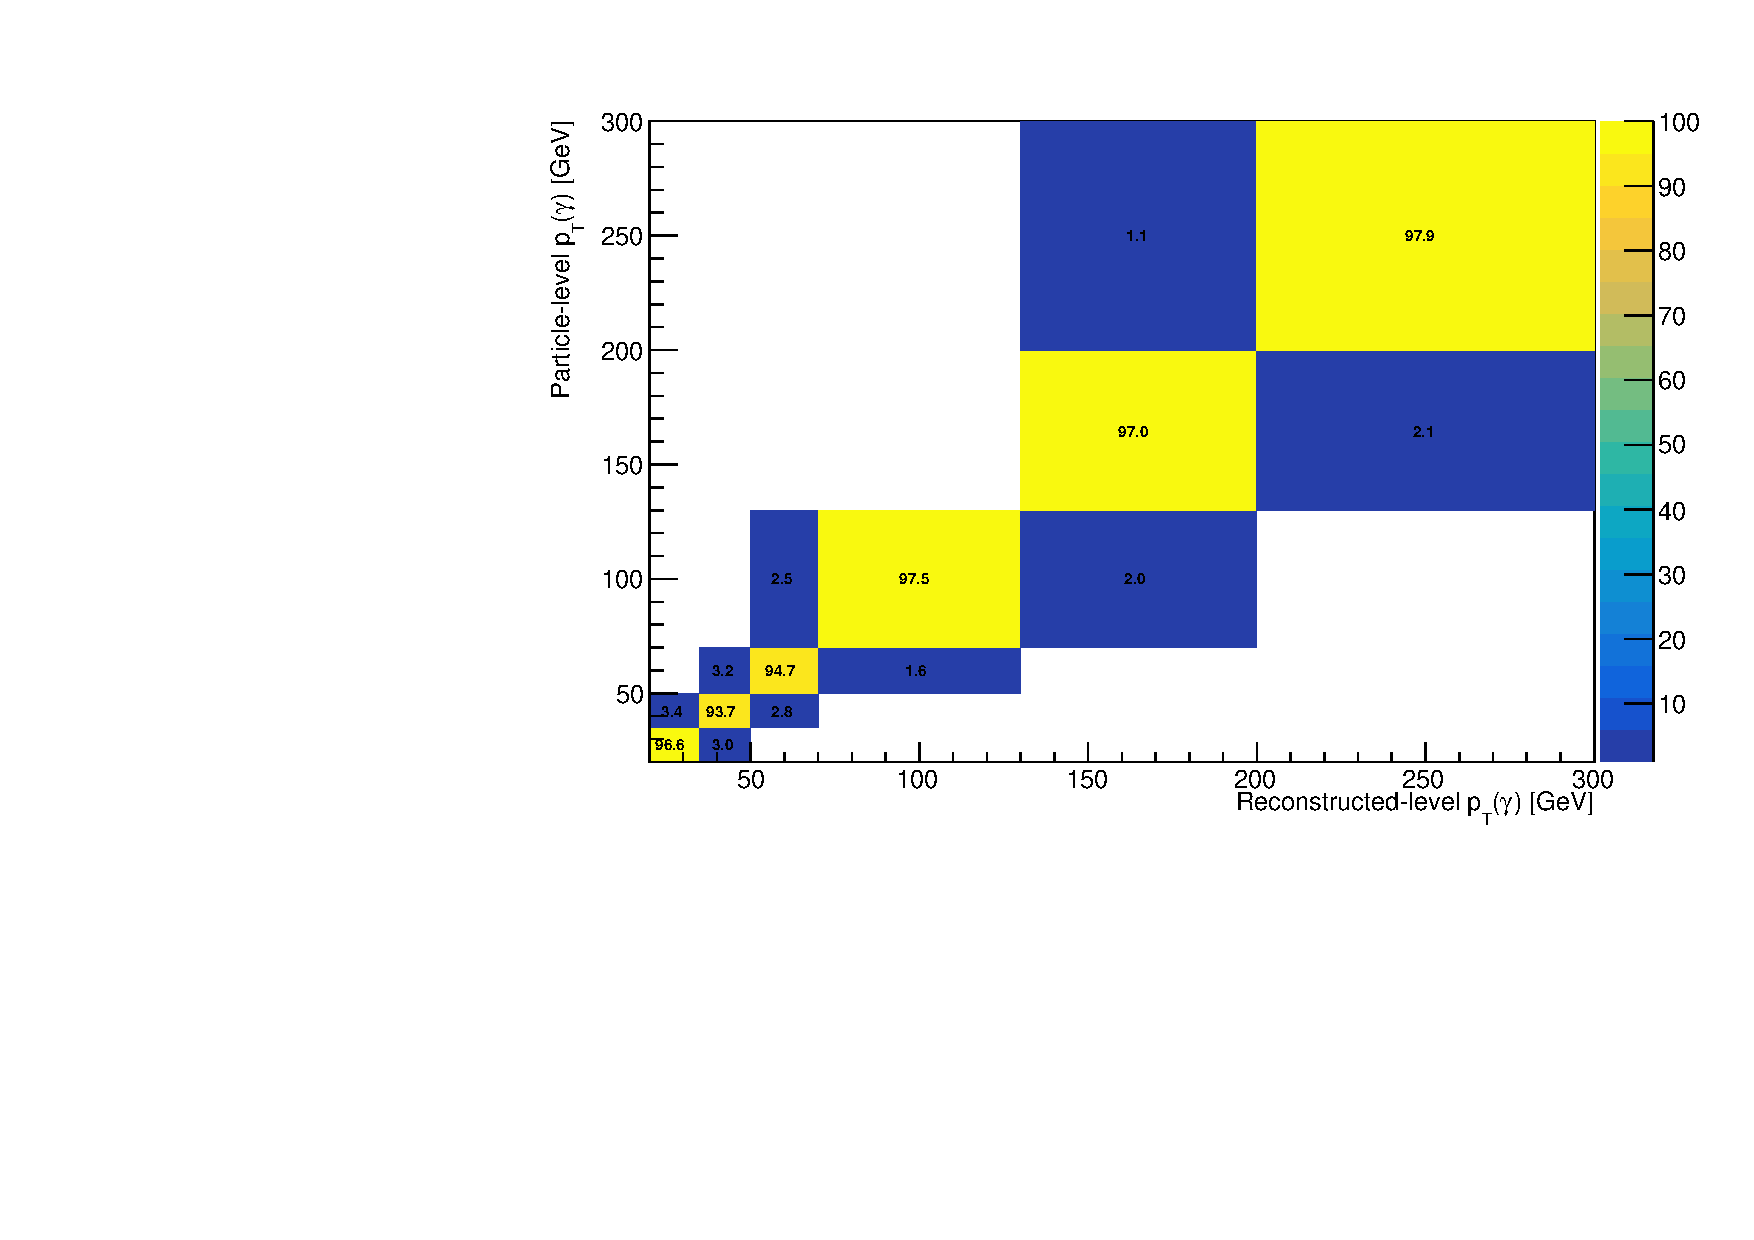
\includegraphics[width=0.4\textwidth]{figures/diff_xsec/dilep/Migration/migration_h2_ph_pt_reco_part_full_weighted_SR1.pdf}}
    \quad\quad
    \subfloat[]{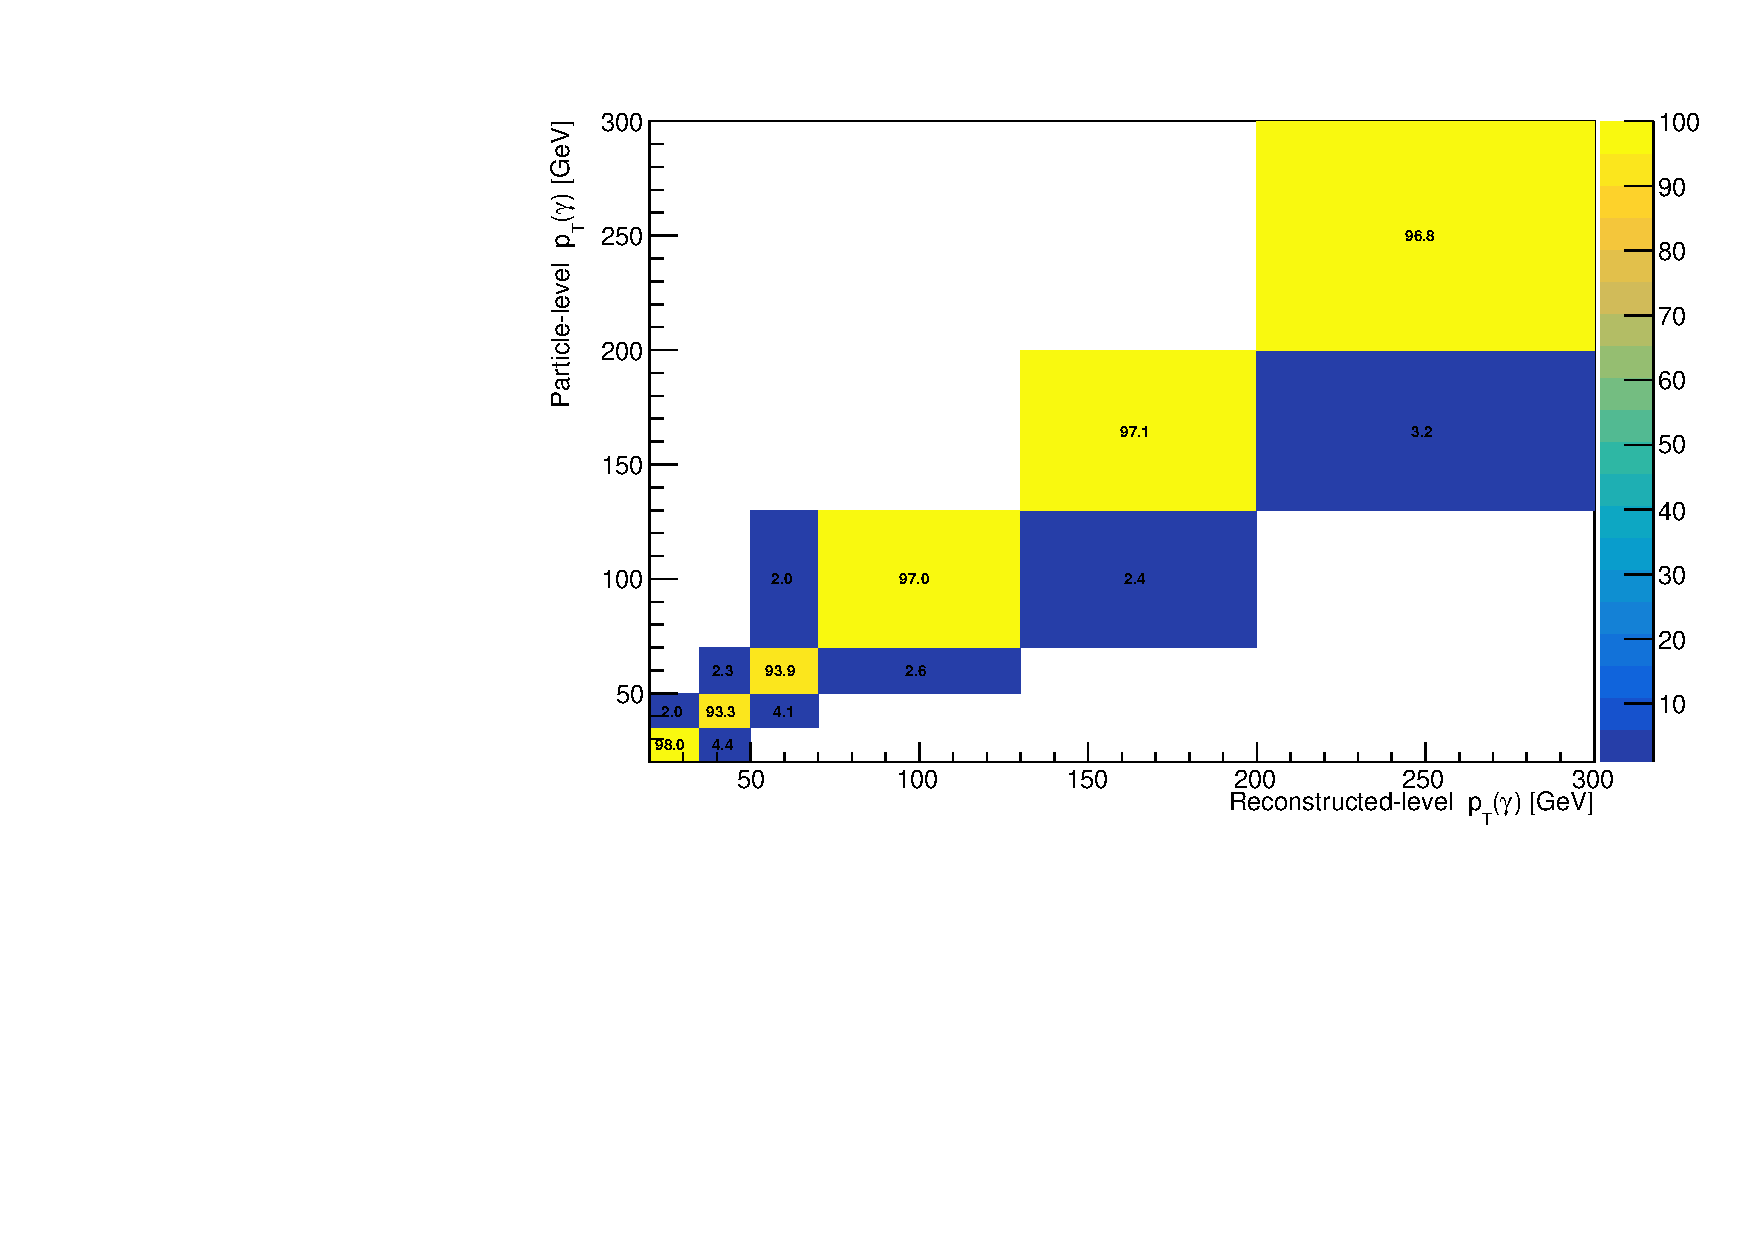
\includegraphics[width=0.4\textwidth]{figures/diff_xsec/dilep/Migration/migration_h2_ph_pt_reco_part_full_weighted_SR2.pdf}}

    \caption{The normalised migration matrices, $M_{\mathrm{r,t}}$ representing the migration of events from the particle level bin to the reconstruction level bin for the two regions defined by the NN output: (a) $O_{\mathrm{NN}} \geq 0.6$ 
    and (b) $O_{\mathrm{NN}} < 0.6$, for the observable $p_T(\gamma)$ in the dilepton channel.}
    \label{fig:folding_input_migration_dilep}
\end{figure}
\FloatBarrier

%%%%%%%%
%  Response matrices dilep
%%%
\begin{figure}[ht]
    \centering
    \subfloat[]{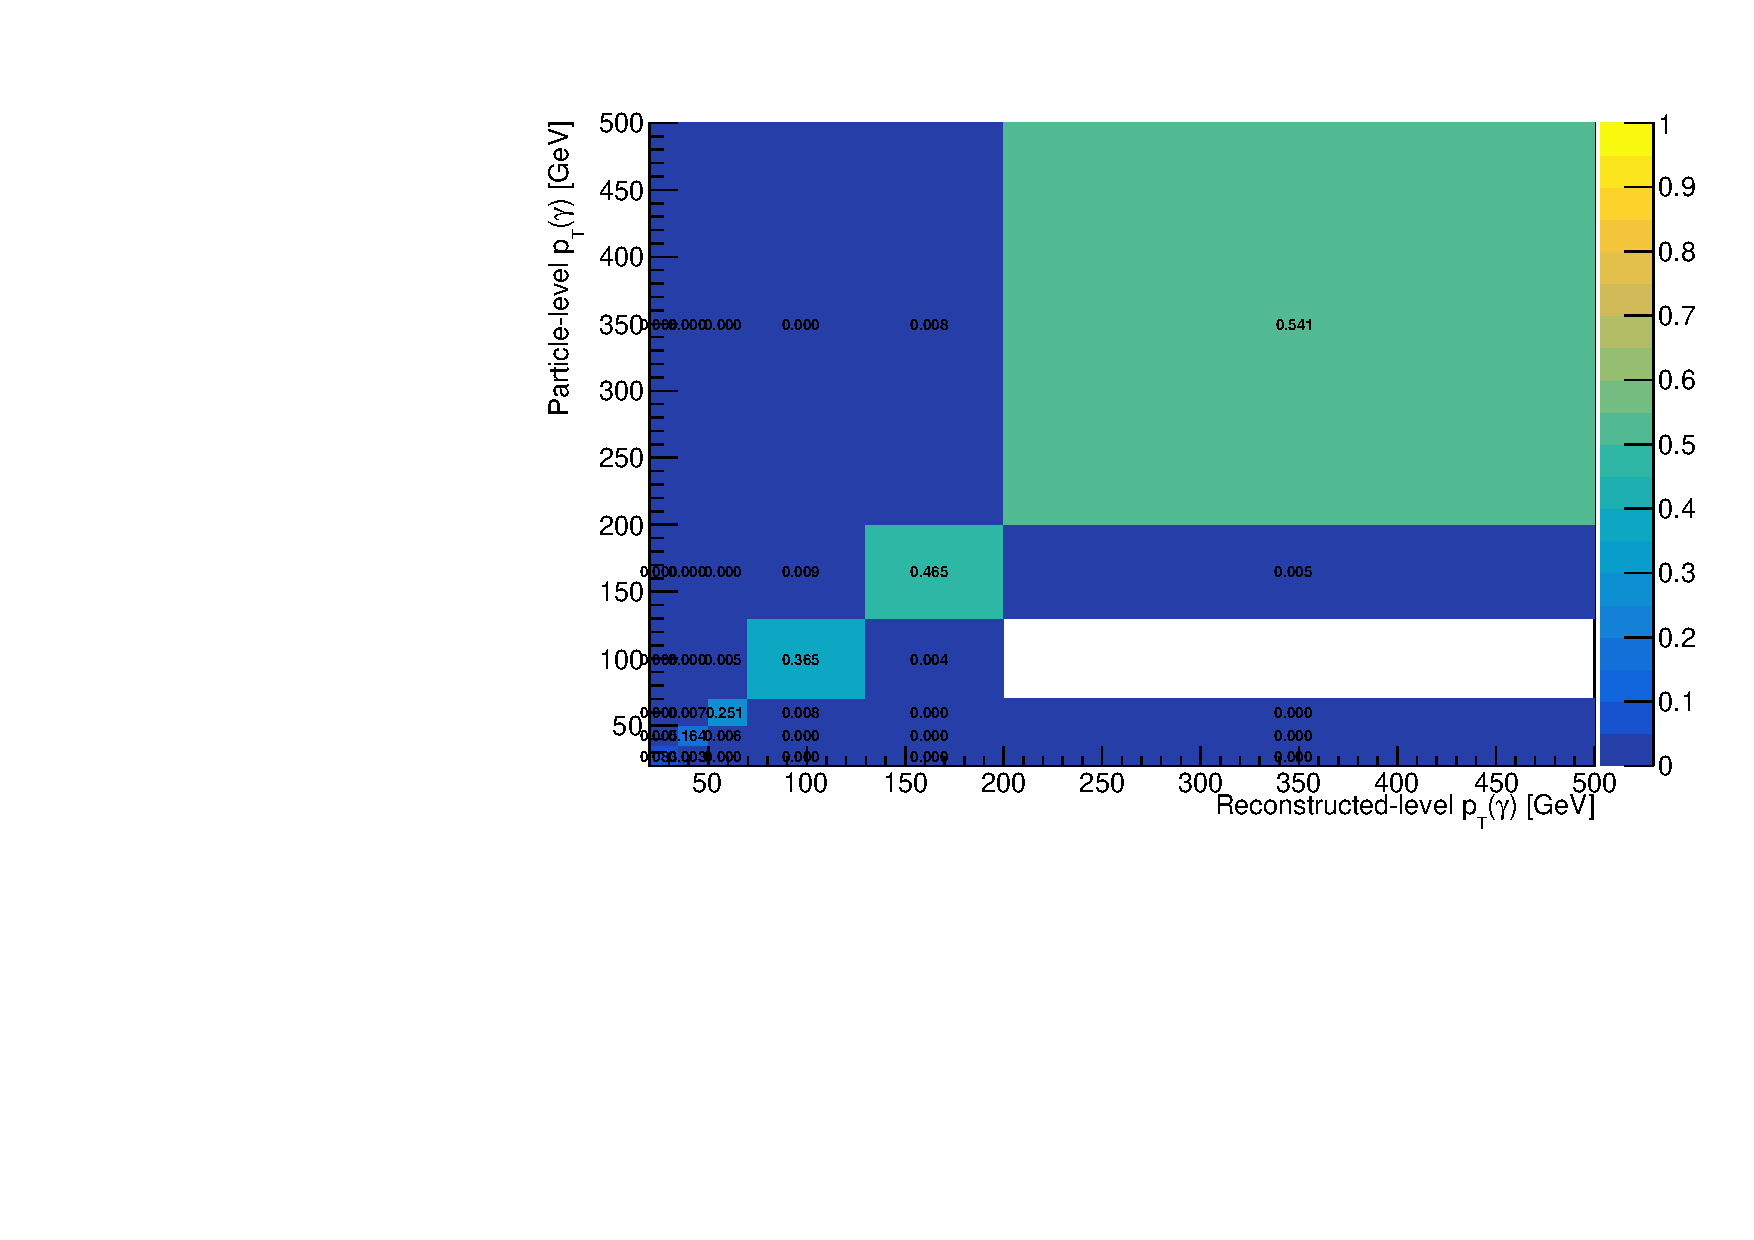
\includegraphics[width=0.4\textwidth]{figures/diff_xsec/dilep/Migration/response_h2_response_matrix_ph_pt_SR1.pdf}}
    \quad\quad
    \subfloat[]{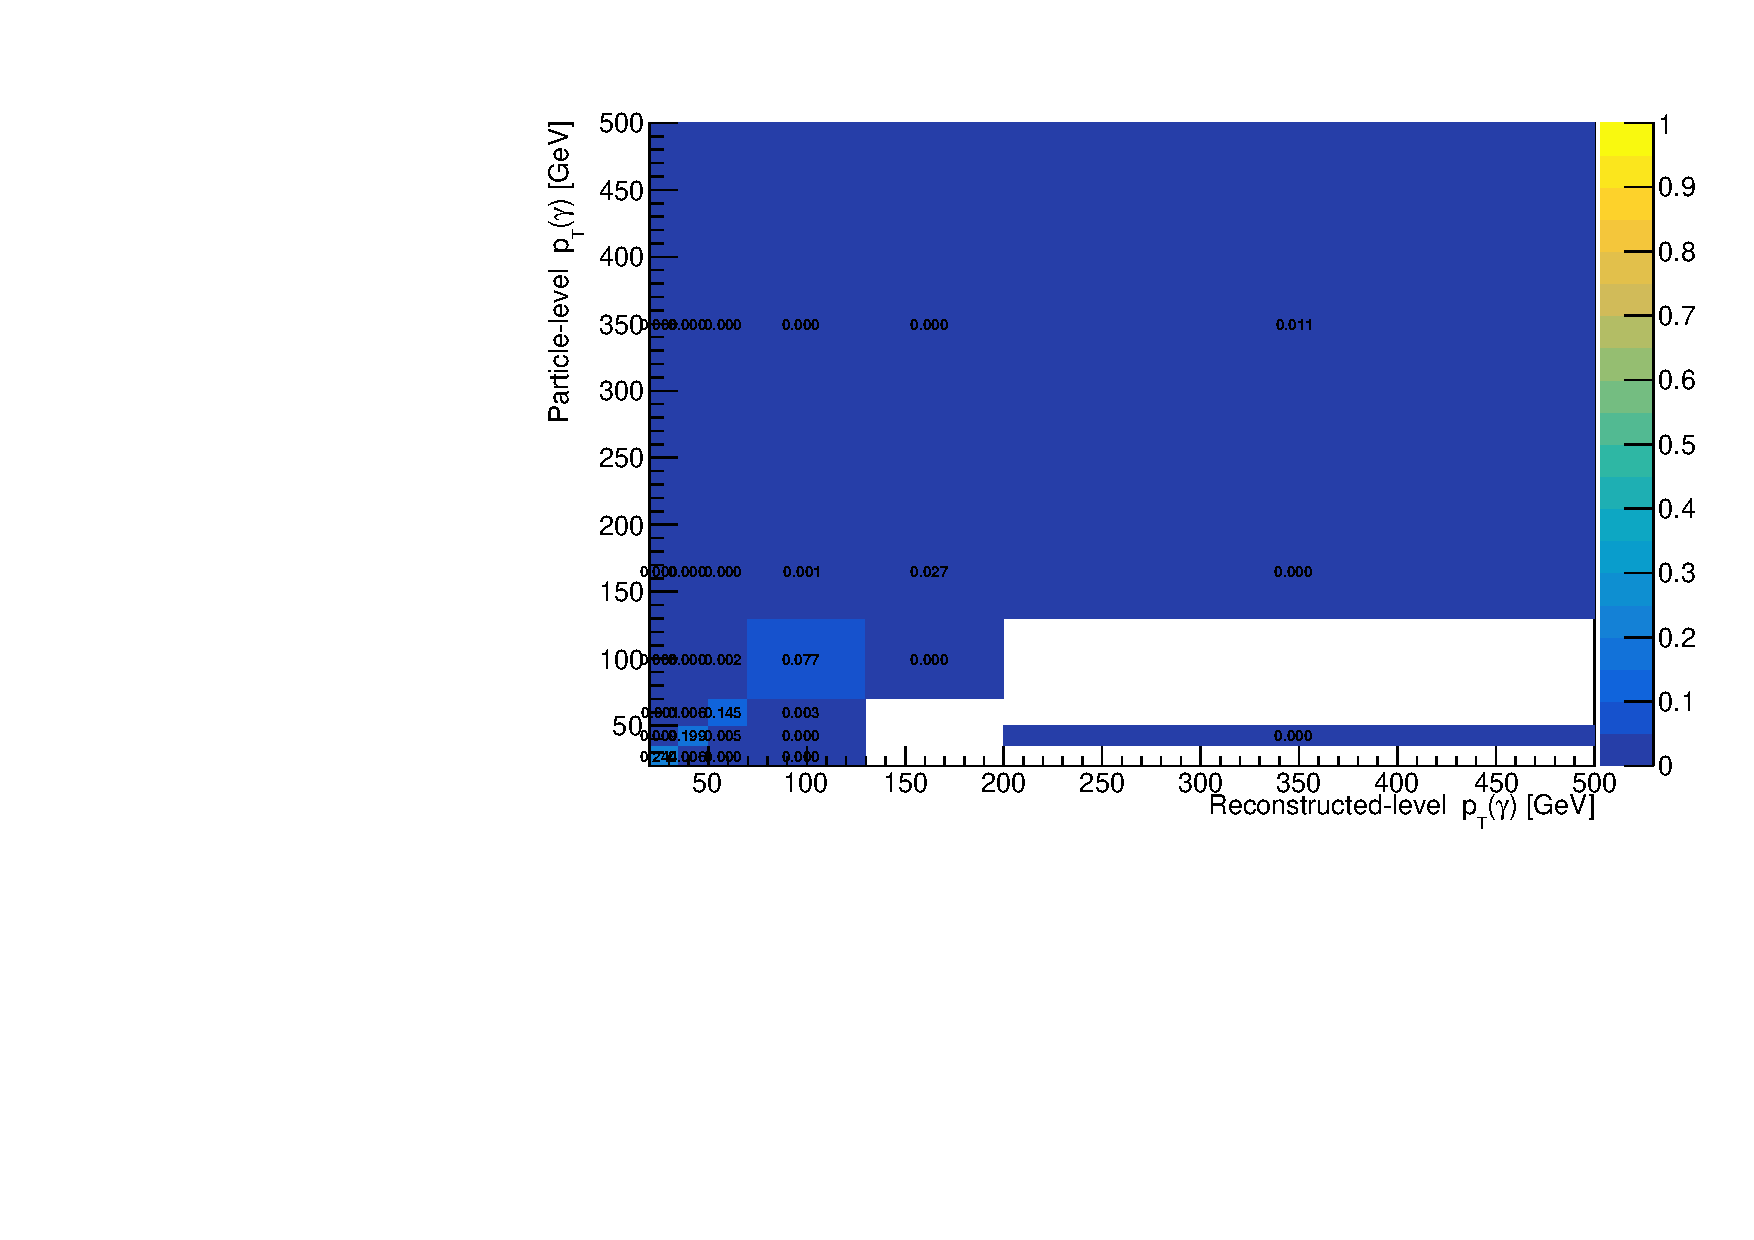
\includegraphics[width=0.4\textwidth]{figures/diff_xsec/dilep/Migration/response_h2_response_matrix_ph_pt_SR2.pdf}}
    \quad\quad
    \subfloat[]{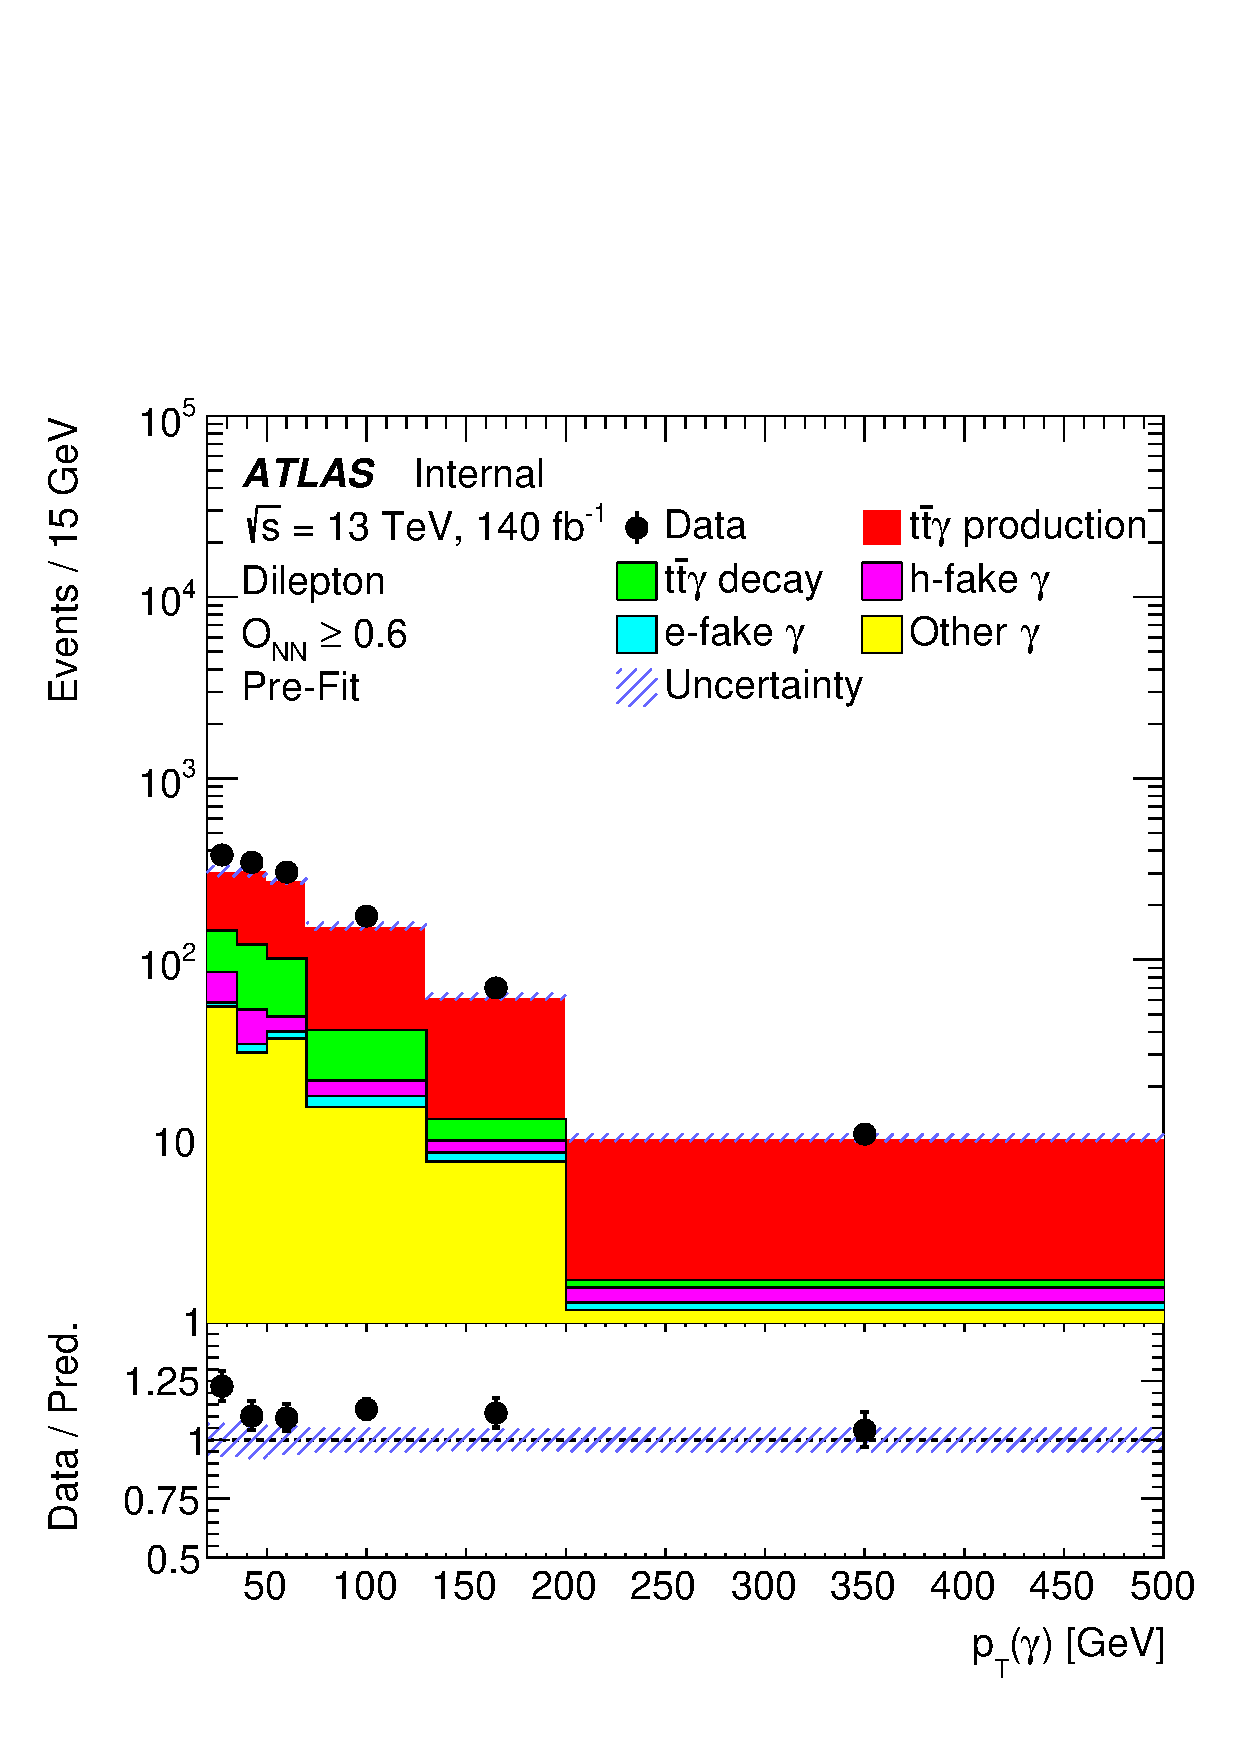
\includegraphics[width=0.4\textwidth]{figures/diff_xsec/dilep/Folded_distributions/tty2l_pt_all_syst/Plots/SR1.pdf}}
    \quad\quad
    \subfloat[]{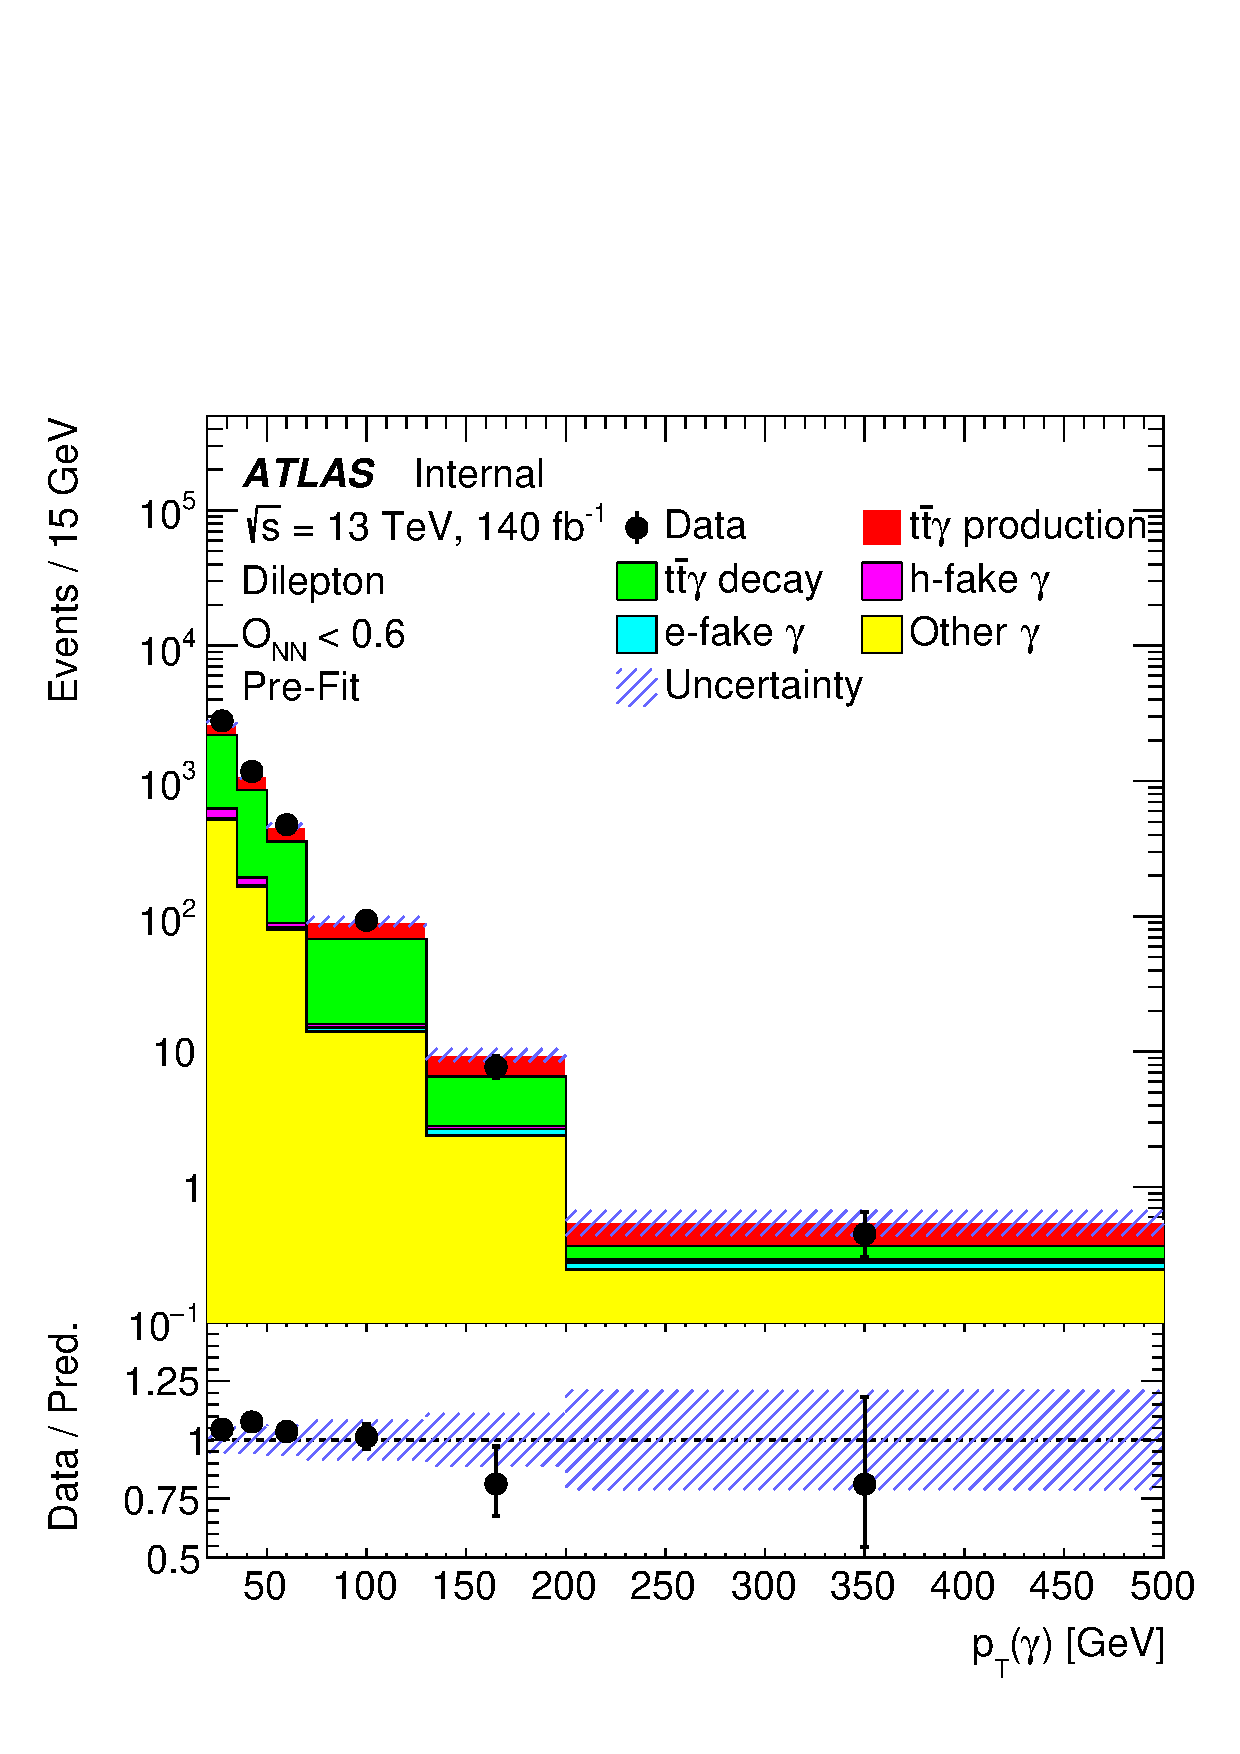
\includegraphics[width=0.4\textwidth]{figures/diff_xsec/dilep/Folded_distributions/tty2l_pt_all_syst/Plots/SR2.pdf}}
    \quad\quad
    \caption{Illustration of response matrices and data-MC comparison plots for
    the observable $p_T(\gamma)$ in dilepton channel. The two regions are
    defined by the Neural Network (NN) output. Subfigures: (a) Response matrix
    for $O_{\mathrm{NN}} \geq 0.6$. (b) Response matrix for $O_{\mathrm{NN}} <
    0.6$. (c) Data-MC comparison for $O_{\mathrm{NN}} \geq 0.6$. (d) Data-MC
    comparison for $O_{\mathrm{NN}} < 0.6$. The signal distribution at the
    reconstruction level is created by folding the truth distribution with the
    corresponding response matrix.}
    \label{fig:folding_input_response_dilep}
\end{figure}
\FloatBarrier

%----------------------------------------------------------------------------------------
%	SECTION 3
%----------------------------------------------------------------------------------------

\section{Results}

Sed ullamcorper quam eu nisl interdum at interdum enim egestas. Aliquam placerat justo sed lectus lobortis ut porta nisl porttitor. Vestibulum mi dolor, lacinia molestie gravida at, tempus vitae ligula. Donec eget quam sapien, in viverra eros. Donec pellentesque justo a massa fringilla non vestibulum metus vestibulum. Vestibulum in orci quis felis tempor lacinia. Vivamus ornare ultrices facilisis. Ut hendrerit volutpat vulputate. Morbi condimentum venenatis augue, id porta ipsum vulputate in. Curabitur luctus tempus justo. Vestibulum risus lectus, adipiscing nec condimentum quis, condimentum nec nisl. Aliquam dictum sagittis velit sed iaculis. Morbi tristique augue sit amet nulla pulvinar id facilisis ligula mollis. Nam elit libero, tincidunt ut aliquam at, molestie in quam. Aenean rhoncus vehicula hendrerit.



